% !TEX root =  centrtutorial.tex

\section{Exact Algorithms}
\begin{frame}
  \frametitle{Outline}
  \begin{enumerate}
    \item Exact algorithms for static graphs
      \begin{enumerate}
        \item the standard algorithm for closeness
        \item the standard algorithm for betweenness
        \item a faster betweenness algorithm through shattering and compression
        \item a GPU-Based algorithm for betweenness
      \end{enumerate}
    \item Exact algorithms for dynamic graphs
      \begin{enumerate}
        \item a dynamic algorithm for closeness
        \item four dynamic algorithms for betweenness
        \item a parallel streaming algorithm for betweenness
      \end{enumerate}
  \end{enumerate}
\end{frame}

\subsection{Exact Algorithms for Static Graphs}

\begin{frame}
  \centering
  \vfill
  {\huge Exact Algorithm for Closeness Centrality}
  \vfill
  {\Large(folklore)}
  \vfill
\end{frame}

\begin{frame}
  \frametitle{Exact Algorithm for Closeness}
    \vfill
    Recall the definition:
    \[
      \closeness(x)=\frac{1}{\sum_{y\neq x}d(x,y)}
    \]
    \vfill
    \pause
    Fastest known algorithm for closeness: \emph{All-Pairs Shortest Paths}
    \begin{itemize}
      \item Runtime: $O(nm+n^2\log n)$
    \end{itemize}
    \vfill
    \pause
    Too slow for \emph{web-scale} graphs!
    \begin{itemize}
      \item Later we'll discuss an \emph{approximation algorithm}
    \end{itemize}
    \vfill
\end{frame}

\begin{frame}
  \centering
  \vfill
  {\huge A Faster Algorithm for Betweenness Centrality}
  \vfill
  {\Large U.~Brandes}
  \vfill
  {\large Journal of Mathematical Sociology (2001)}
  \vfill
\end{frame}

\begin{frame}
  \frametitle{Why {\red faster}?}
  \vfill
  Let's take a step back. Recall the definition
  \[
    \sum_{\substack{s\neq x\neq t \in V\\s\neq t}}\frac{\sigma_{st}(x)}{\sigma_{st}}
    \vspace{-10pt}
  \]
  \begin{itemize}
    \item $\sigma_{st}$: no.~of \spath (SPs) from $s$ to $t$
    \item $\sigma_{st}(x)$: no.~of \spath from $s$ to $t$ that go through $x$
  \end{itemize}
  \pause
  We could:
  \begin{enumerate}
    \item obtain all the $\sigma_{st}$ and $\sigma_{st}(x)$ for all $x$, $s$,
      $t$ via APSP; and then
    \item perform the aggregation to obtain $\betw(x)$ for all $x$.
  \end{enumerate}
  \pause
  The first step takes $O(nm+n^2\log n)$, but the second step takes\ldots\pause
  $\Theta(n^3)$ (a sum of $O(n^2)$ terms for each of the $n$ vertices).
  \pause
  \vfill
  Brandes' algorithm interleaves the SP computation with the aggregation,
  achieving runtime $O(nm+n^2\log n)$\\
  \quad I.e., it is \emph{faster} than the APSP approach
\end{frame}

\begin{frame}
  \frametitle{Dependencies}
  Define: \emph{Dependency} of $s$ on $v$:
  \[
    \dep_s(v)=\sum_{t\neq s\neq v}\frac{\sigma_{st}(v)}{\sigma_{st}}
  \]
  Hence:
  \[
    \betw(v)=\sum_{s\neq v}\dep_s(v)
  \]
  \pause
  Brandes proved that $\delta_s(v)$ obeys a \emph{recursive relation}:
  \[
    \dep_s(v)=\sum_{w:v\in\pred_s(w)}\frac{\sigma_{sv}}{\sigma_{sw}}\left(1+\dep_s(w)\right)
  \]
  We can leverage this relation for efficient computation of betweenness
\end{frame}

\begin{frame}
  \frametitle{Recursive relation}
  \begin{theorem}[Simpler form]
    If there is exactly one \spath from $s$ to each $t$, then
    \[
      \dep_s(v)=\sum_{w: v\in\pred_s(w)}\left(1+\dep_s(w)\right)
    \]
  \end{theorem}
  \pause
  \emph{Proof sketch:}
  \begin{itemize}
    \item The \spdag from $s$ is a tree;
    \item Fix $t$. $v$ is either on the single \spath from $s$ to $t$ or not.
    \item $v$ lies on all and only the SPs to vertices $w$ for which $v$ is a
      predecessor (one \spath for each $w$) and the SPs that these lie on. Hence the
      thesis.
  \end{itemize}
  \pause
  The general version must take into account that not all SPs from $s$ to $w$ go
  trough $v$.
\end{frame}

\begin{frame}
  \frametitle{Brandes' Algorithm}
  \begin{enumerate}
    \item Initialize $\dep_s(v)$ to $0$ for each $v,s$ and $\betw(w)$ to $0$ for
      each $w$.
    \item Iterate the following loop for each vertex $s$:
      \begin{enumerate}
        \item Run Dijkstra's algorithm from $s$, keeping track of $\sigma_{sv}$ for
          each encountered vertex $v$, and inserting the vertices in a max-heap $H$ by
          distance from $s$;
        \item While $H$ is not empty:
          \begin{enumerate}
            \item Pop the max vertex $t$ in $H$;
            \item For each $w\in\pred_s(t)$, increment $\dep_s(w)$ by
              $\frac{\sigma_{sw}}{\sigma_{st}}(1+\dep_s(t))$;
            \item Increment $\betw(t)$ by $\dep_s(t)$;
          \end{enumerate}
      \end{enumerate}
  \end{enumerate}
\end{frame}

\begin{frame}
  \centering
  \vfill
  {\huge Shattering and Compressing Networks for Betweenness Centrality}
  \vfill
  {\Large A.~E.~Sar\i y\"uce, E.~Saule, K.~Kaya, \"U.~V.~\c{C}ataly\"urek}
  \vfill
  {\large SDM '13: SIAM Conference on Data Mining}
  \vfill
\end{frame}

\begin{frame}
  \frametitle{Intuition}
  \emph{Observations:}
  \begin{itemize}
    \item There are vertices with predictable betweenness (e.g., 0, or equal to one
      of their neighbors). We can remove them from the graph (\emph{compression})
    \item Partitioning the (compressed) graph into small components allows for
      faster SP computation (\emph{shattering})
  \end{itemize}
  \pause
  \emph{Idea}:
  We can iteratively compress \& shatter until we can't reduce the graph any
  more.\\
  \qquad Only at this point we run (a modified) Brandes's algorithm and then
  aggregate the ``partial'' betweenness in different components.
\end{frame}

\begin{frame}
  \frametitle{Introductory definitions}
  \vfill
  \begin{itemize}
    \item Graph $G=(V,E)$
    \item \emph{Induced graph} by $V'\subseteq V$: $G_{V'}=(V', E'=V'\times V'\cap E)$
    \pause
    \item Neighborhood of a vertex $v$: $\neighbors(v)=\{u~:~(v,u)\in E\}$
    \pause
  \item \emph{Side vertex}: a vertex $v$ such that $G_{\neighbors(v)}$ is a clique
    \pause
  \item \emph{Identical vertices}: two vertices $u$ and $v$ such that either
      $\neighbors(u)=\neighbors(v)$ or
      $\neighbors(u)\cup\{u\}=\neighbors(v)\cup\{v\}$
  \end{itemize}
  \vfill
\end{frame}


\begin{frame}
  \frametitle{Compression}
  \vfill
  Empirical / intuitive observations
  \begin{itemize}
    \item if $v$ has degree $1$, then $\betw(v)=0$
    \item if $v$ is a side vertex, then $\betw(v)=0$
    \item if $u$ and $v$ are identical, then $\betw(v)=\betw(w)$
  \end{itemize}
  \pause
  \vfill
  \emph{Compression}:
  \begin{itemize}
    \item remove degree-1 vertices and side vertices; and
    \item merge identical vertices
  \end{itemize}
  \vfill
\end{frame}

\begin{frame}
  \frametitle{Shattering}
  \vfill
  \begin{itemize}
    \item \emph{Articulation vertex}: vertex $v$ whose deletion makes the graph disconnected
    \item \emph{Bridge edge:} an edge $e=(u,v)$ such that $G'=(V,E\setminus\{e\})$ has
      more components than $G$ ($u$ and $v$ are articulation vertexes)
  \end{itemize}
  \pause
  \vfill
  \emph{Shattering}:
  \begin{itemize}
    \item remove bridge edges
    \item split articulation vertices in two copies, one per resulting component
  \end{itemize}
\end{frame}

\begin{frame}
  \frametitle{Example of shattering and compression}
  \begin{figure}
    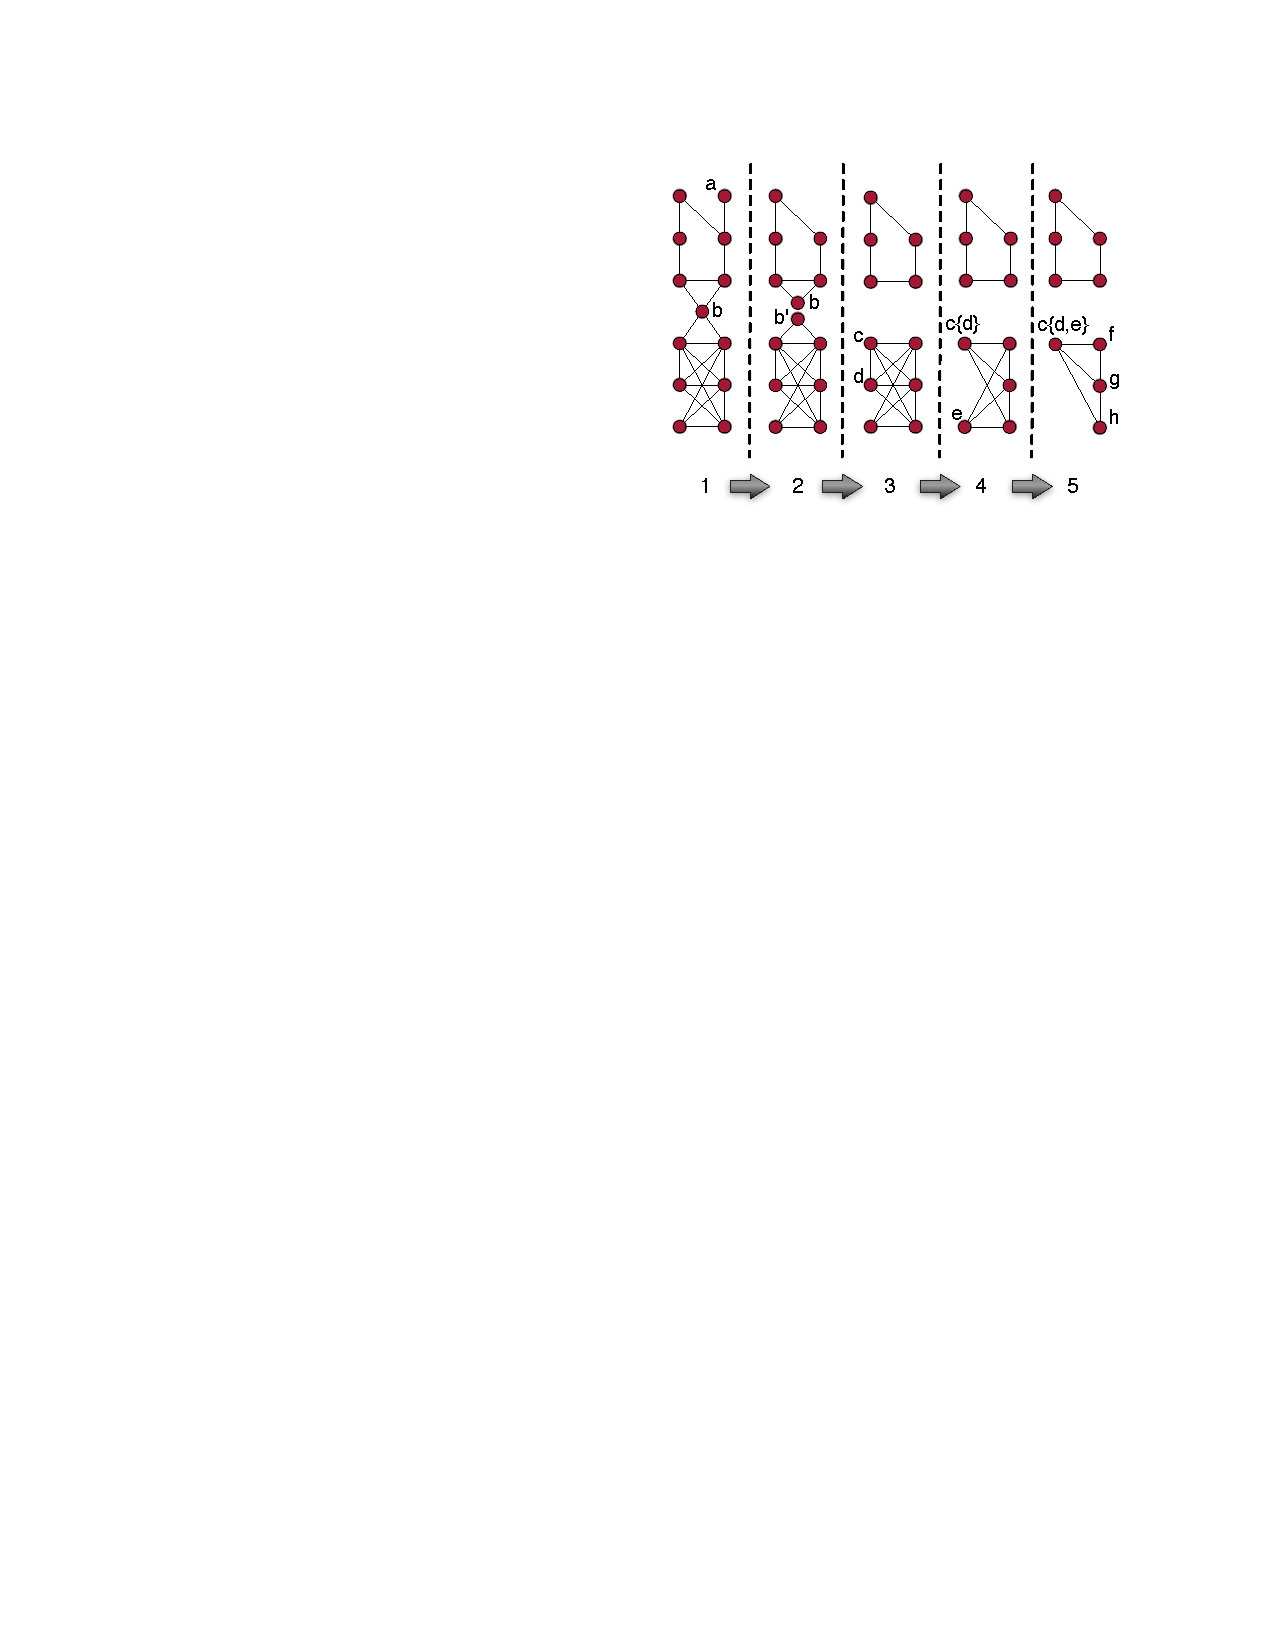
\includegraphics{imgs/shatteringbadios.pdf}
  \end{figure}
\end{frame}

\begin{frame}
  \frametitle{Issues}
  Issues to take care of when iteratively compressing \& shattering:
  \begin{block}{Example of issue}
    A vertex may have degree 1 only after we removed another vertex: we can't
    just remove and forget it, as its original betweenness was not 0.
  \end{block}
  \pause
  \begin{block}{Example of issue}
    When splitting an articulation vertex into component copies, we need to know,
    for each copy, how many vertices in other components are reachable through
    that vertex.
  \end{block}
  ...and more
\end{frame}

\begin{frame}
  \frametitle{Solution}
  (Sketch)
  \begin{itemize}
    \item When we remove a vertex $u$, one of its neighbors (or an identical vertex)
      $v$ is elected as the representative for $u$ (and for all vertices that $u$
      was a representative of)
    \item We adjust the (current) values of $\betw(v)$ and $\betw(u)$ to
      appropriately take into account the removal of $u$\\
      \qquad the details are too hairy for a talk\ldots
    \item When splitting articulation vertices or removing bridges, similar
      adjustments take place
    \item Brandes' algorithm is slightly modified to take the number of vertices
      that a vertex represents into consideration when computing the
      dependencies and the betweenness values
  \end{itemize}
\end{frame}

\begin{frame}
  \frametitle{Speedup}
  ``org.'' is Brandes' algorithm, ``best'' is compress \& shatter
  \begin{figure}
    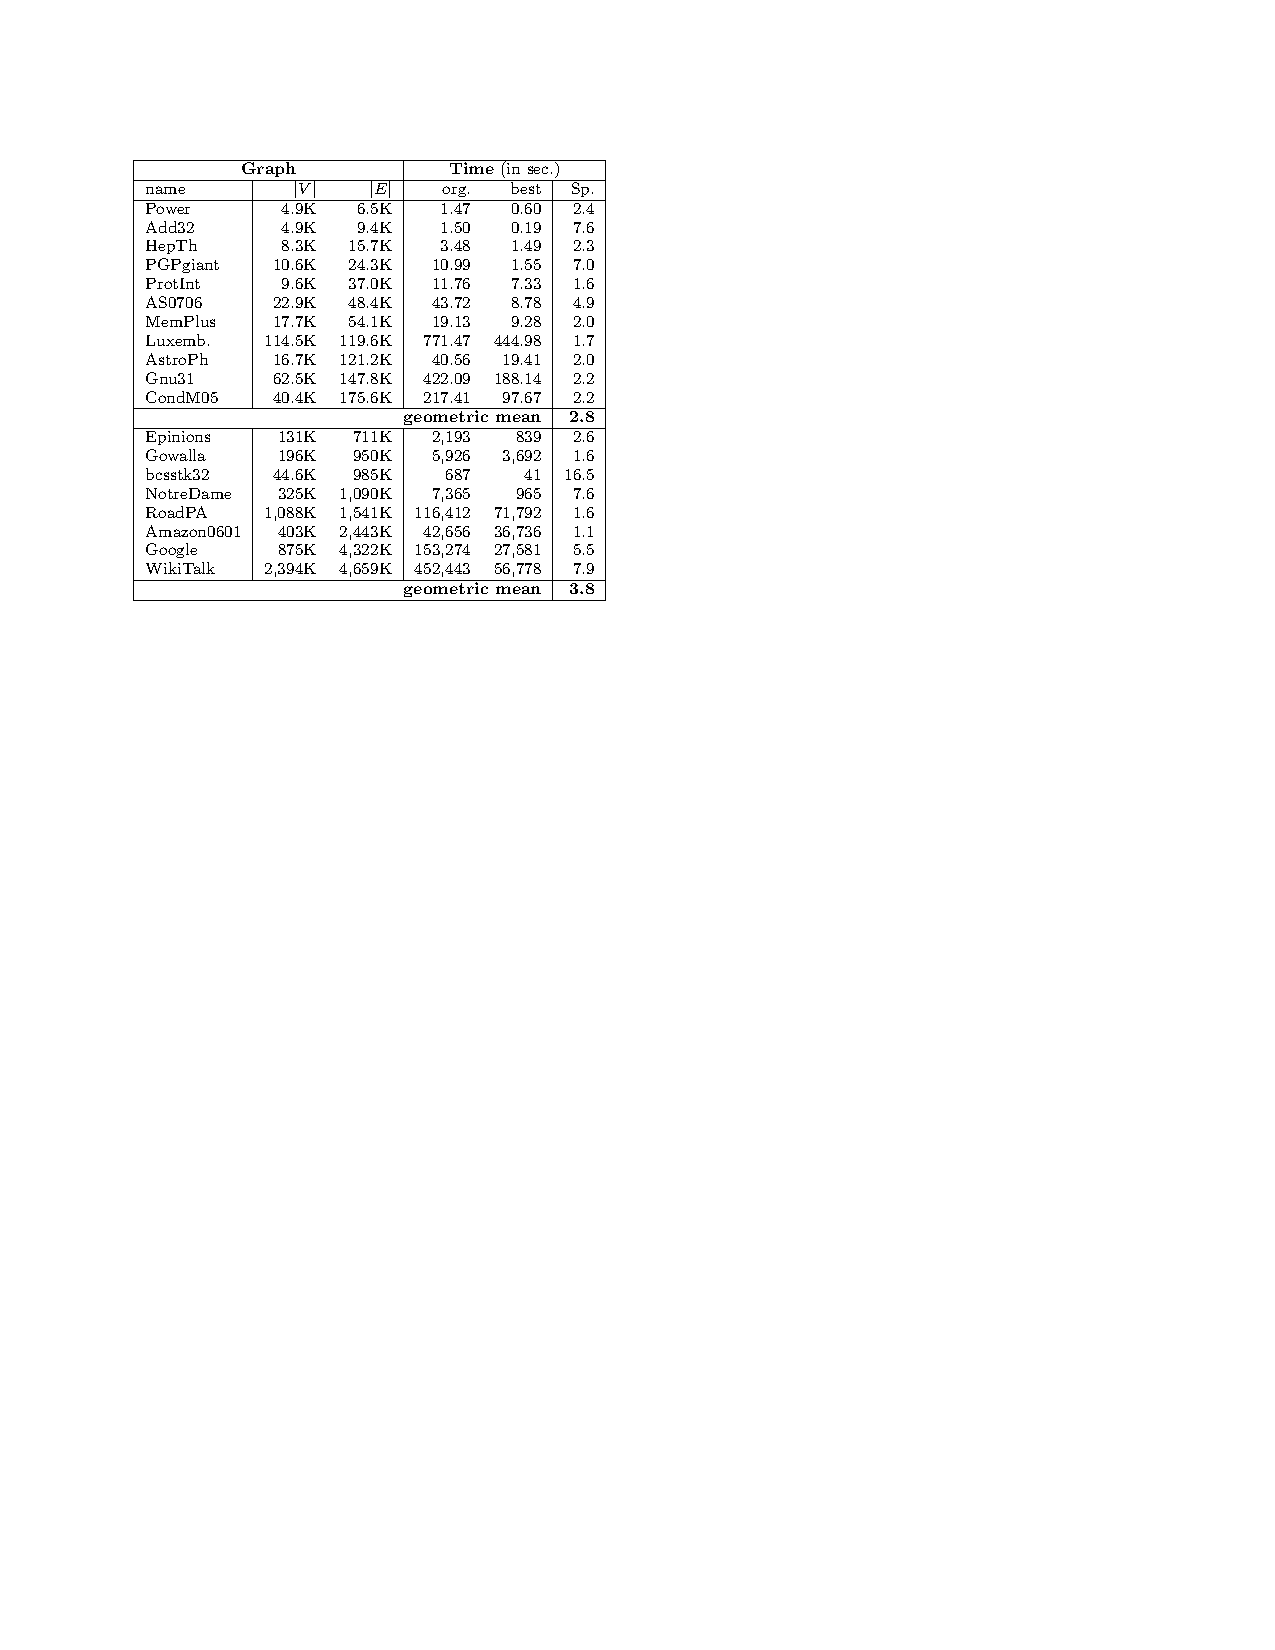
\includegraphics{imgs/runtimebadios.pdf}
  \end{figure}
\end{frame}

\begin{frame}
  \frametitle{Composition of runtime}
  \begin{itemize}
    \item Preproc is the time needed to compress \& shatter, Phase 1 is SSSP,
      Phase 2 is aggregation
    \item Different column for different variants of the algorithm (e.g., only
      compression of 1-degree vertices, only shattering of edges)
    \item the lower the better
  \end{itemize}
  \begin{figure}
    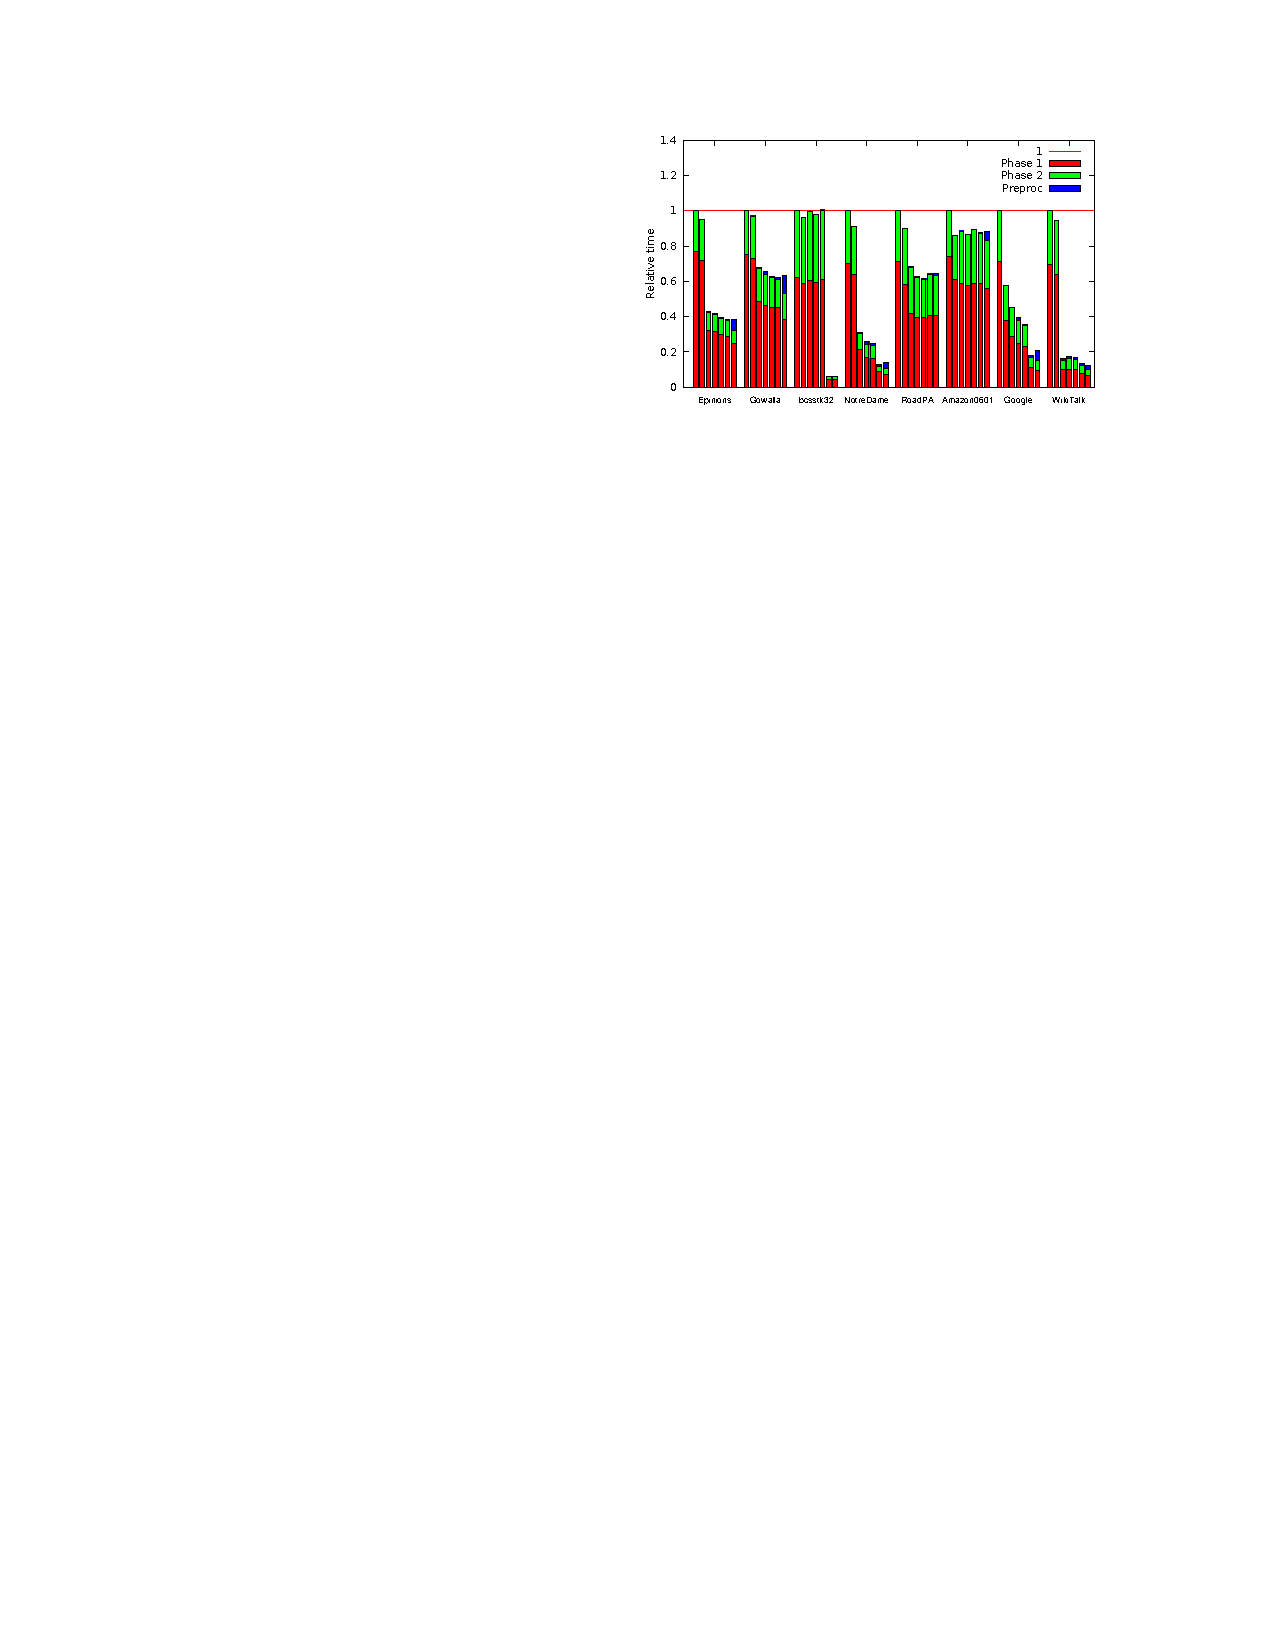
\includegraphics[width=0.9\textwidth]{imgs/runtimesplitbadios.pdf}
  \end{figure}
\end{frame}

%\begin{frame}
%  \frametitle{A Divide-and-Conquer Algorithm for Betweenness Centrality}
%  \centering
%  \vfill
%  {\huge D.~Erd\H{o}s, V.~Ishakian, A.~Bestravros, E.~Terzi}
%  \vfill
%  {\large SIAM Data Mining Conference (2015)}
%\end{frame}

%% Sariyüce et al.
\begin{frame}
  \centering
  \vfill
  {\huge Betweenness Centrality on GPUs and Heterogeneous Architectures}
  \vfill
  {\Large A.~E.~Sar\i y\"uce, K.~Kaya, E.~Saule, \"U.~V.~\c{C}ataly\"urek}
  \vfill
  {\large GPGPU '13: Workshop on General Purpose Processing Using GPUs}
  \vfill
\end{frame}

\begin{frame}
  \frametitle{Parallelism}

  \begin{itemize}
    \item Fine grained: single concurrent BFS
    \item Only one copy of auxiliary data structures
    \item Synchronization needed
    \item Better for GPUs, which have small memory
  \end{itemize}
  \begin{itemize}
    \item Coarse grained: many independent BFSs
    \item Sources are independent, embarrassingly parallel
    \item More memory needed
    \item Better for CPUs, which have large memory
  \end{itemize}
\end{frame}

\begin{frame}
  \frametitle{GPU}

  \begin{quote}
    A GPU is especially well-suited to address problems that can be expressed as \textbf{data-parallel computations} - the same program is executed on many data elements in parallel - with \textbf{high arithmetic intensity} - the ratio of arithmetic operations to memory operations.

    Because the same program is executed for each data element, there is a lower requirement for sophisticated flow control, and because it is executed on many data elements and has high arithmetic intensity, the memory access latency can be hidden with calculations instead of big data caches.\footnote{\url{docs.nvidia.com/cuda/cuda-c-programming-guide/index.html}}
  \end{quote}
\end{frame}


\begin{frame}
  \frametitle{Execution model}
  \begin{columns}[onlytextwidth]

    \begin{column}{0.5\textwidth}
      \begin{itemize}
        \item One thread per data element
        \item Thread scheduled in blocks with barriers (wait for others at the end)
        \item Program runs on the whole data (kernel)
      \end{itemize}
      \begin{itemize}
        \item Minimize synchronization
        \item Balance load
        \item Coalesce memory access
      \end{itemize}
    \end{column}

    \begin{column}{0.5\textwidth}
      \begin{figure}[t]
        \centering
        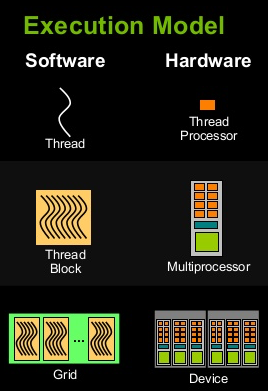
\includegraphics[width=\textwidth, height=0.8\textheight, keepaspectratio]{imgs/cuda}
      \end{figure}
    \end{column}
  \end{columns}

\end{frame}


\begin{frame}
  \frametitle{Intuition}

  \begin{itemize}
    \item GPUs have huge number of cores
    \item Use them to parallelize BFS
    \item One core per vertex, or one core per edge
    \item Vertex-based parallelism creates load imbalance for graphs with skewed degree distribution
    \item Edge-based parallelism requires high memory usage
  \end{itemize}
  \begin{itemize}
    \item Use vertex-based parallelism
    \item Virtualize high-degree vertices to address load imbalance
    \item Reduce memory usage by removing predecessors lists
  \end{itemize}

\end{frame}


\begin{frame}
  \frametitle{Difference}

  \begin{columns}[onlytextwidth]
    \begin{column}{0.5\textwidth}
      \begin{figure}[t]
        \centering
        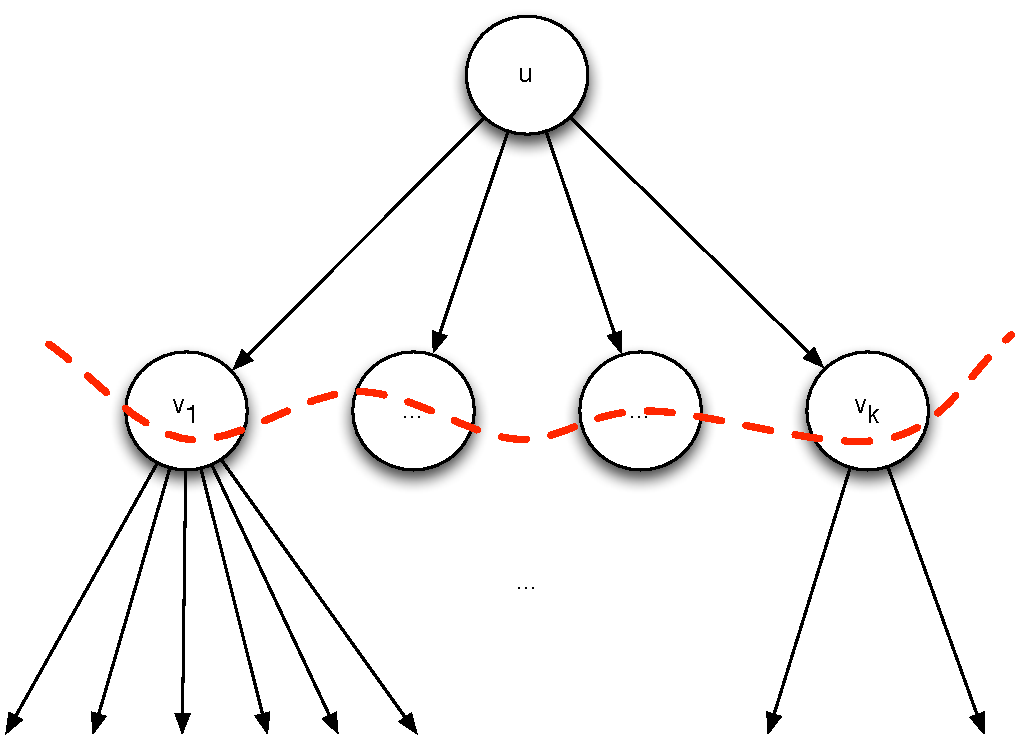
\includegraphics[width=\textwidth, height=0.6\textheight, keepaspectratio]{imgs/gpu-vertex-bfs}
        \caption{Vertex-based BFS}
      \end{figure}
    \end{column}

    \begin{column}{0.5\textwidth}
      \begin{figure}[t]
        \centering
        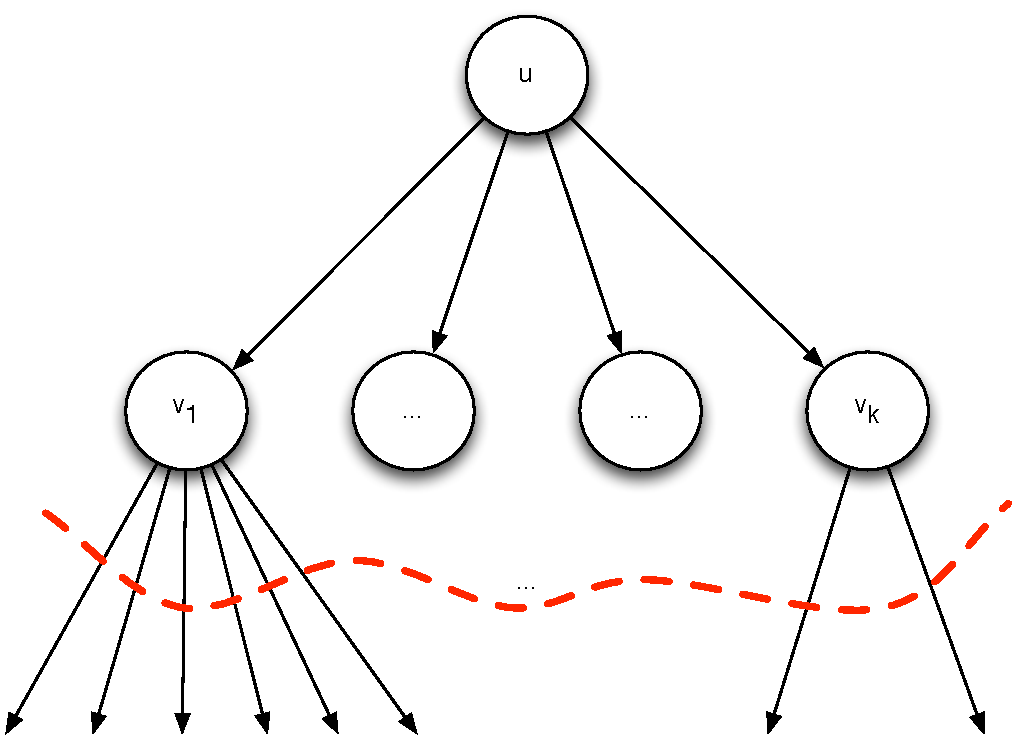
\includegraphics[width=\textwidth, height=0.6\textheight, keepaspectratio]{imgs/gpu-edge-bfs}
        \caption{Edge-based BFS}
      \end{figure}
    \end{column}
  \end{columns}

\end{frame}


\begin{frame}
  \frametitle{Vertex-based}

  \begin{columns}[onlytextwidth]
    \begin{column}{0.5\textwidth}
      \begin{itemize}
        \item For each level, for each vertex in parallel
        \item If vertex is on level
        \item For each neighbor, \\ adjust \pred and \paths
        \item Atomic update on \paths needed (multiple paths can be discovered concurrently)
        \item While backtracking, if $u \in \pred(v)$ accumulate $\dep(u) = \dep(u) + \dep(v)$
        \item Possible load imbalance if degree skewed
      \end{itemize}
    \end{column}

    \begin{column}{0.5\textwidth}
      \begin{figure}[t]
        \centering
        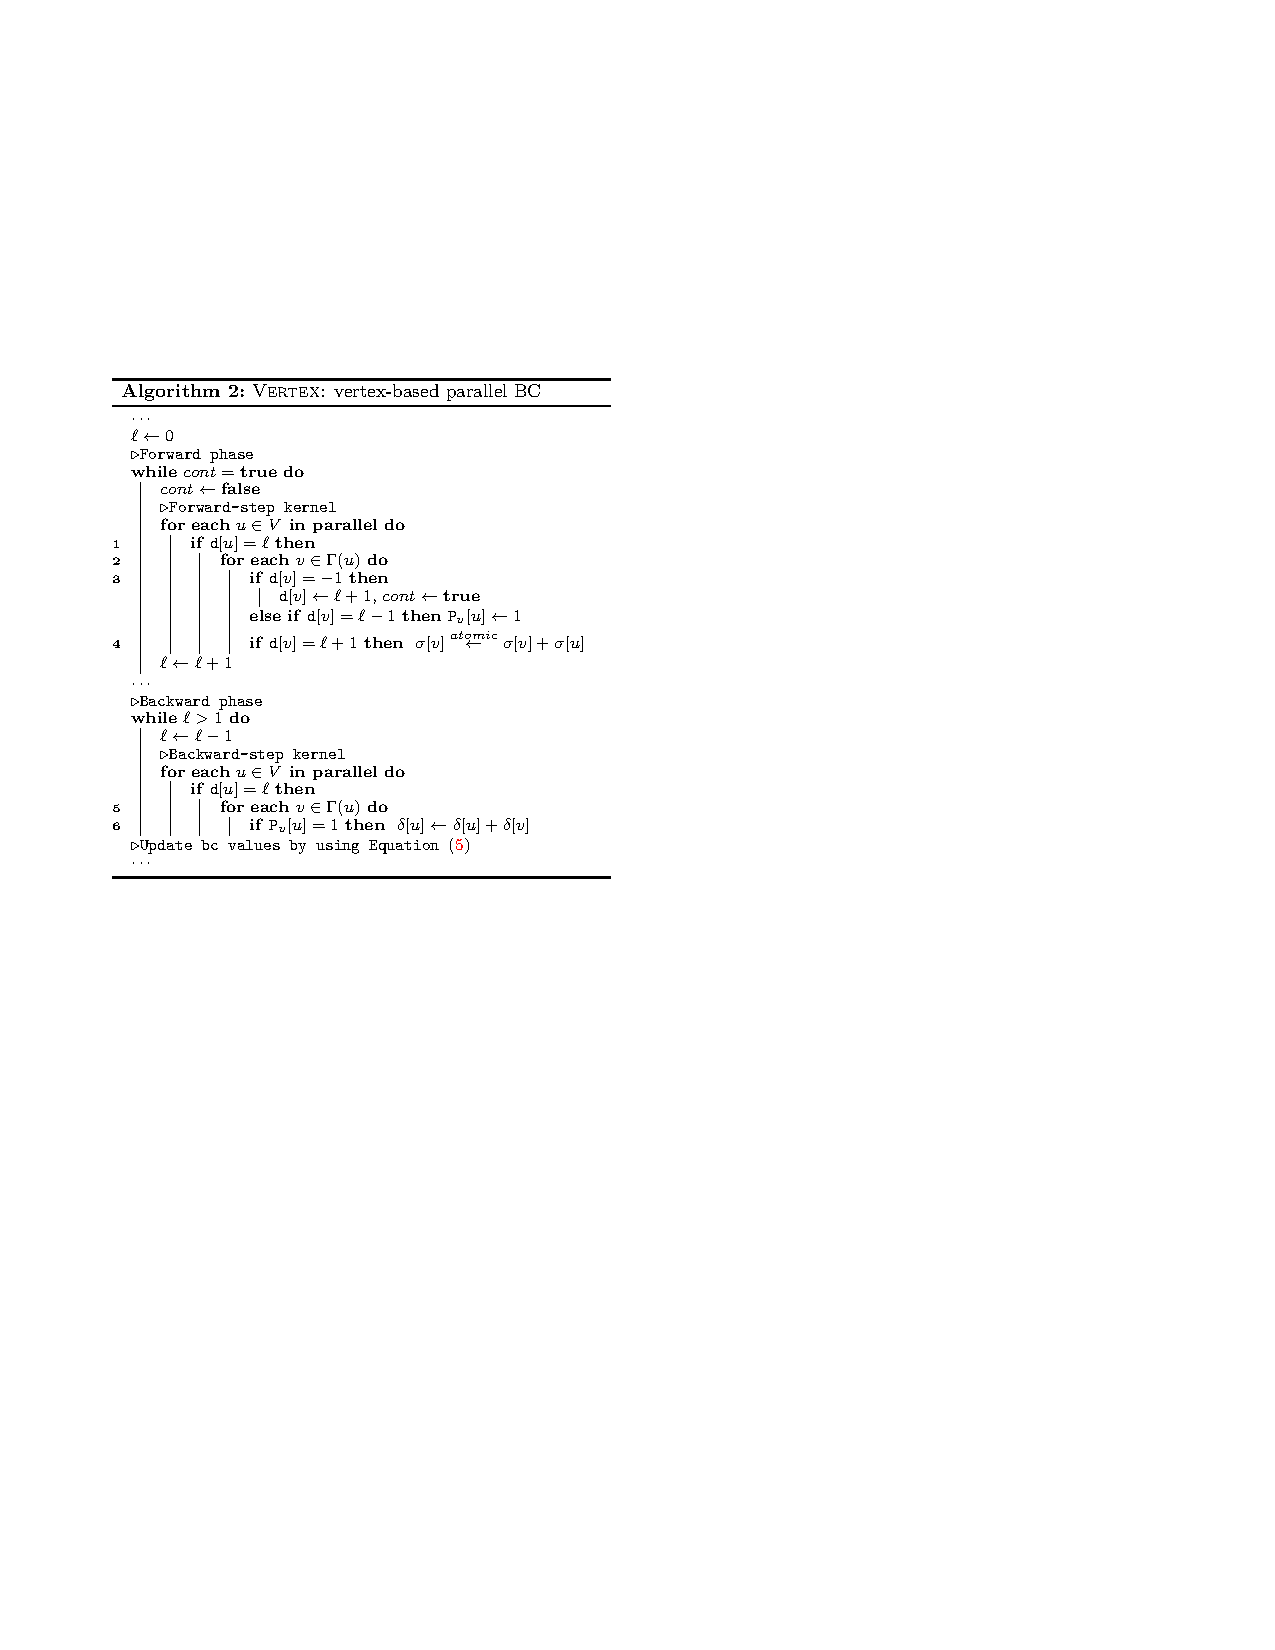
\includegraphics[width=\textwidth, height=0.8\textheight, keepaspectratio]{imgs/gpu-algo-vertex}
      \end{figure}
    \end{column}
  \end{columns}

\end{frame}


\begin{frame}
  \frametitle{Edge-based}

  \begin{columns}[onlytextwidth]
    \begin{column}{0.5\textwidth}
      \begin{itemize}
        \item For each level, for each edge in parallel
        \item If edge endpoint is on level
        \item Same as above...
        \item While backtracking, if $u \in \pred(v)$ accumulate $\dep(u) = \dep(u) + \dep(v)$ \emph{atomically}
        \item Multiple edges can try to update \dep concurrently
        \item More memory (edge-based layout) and more atomic operations
      \end{itemize}
    \end{column}

    \begin{column}{0.5\textwidth}
      \begin{figure}[t]
        \centering
        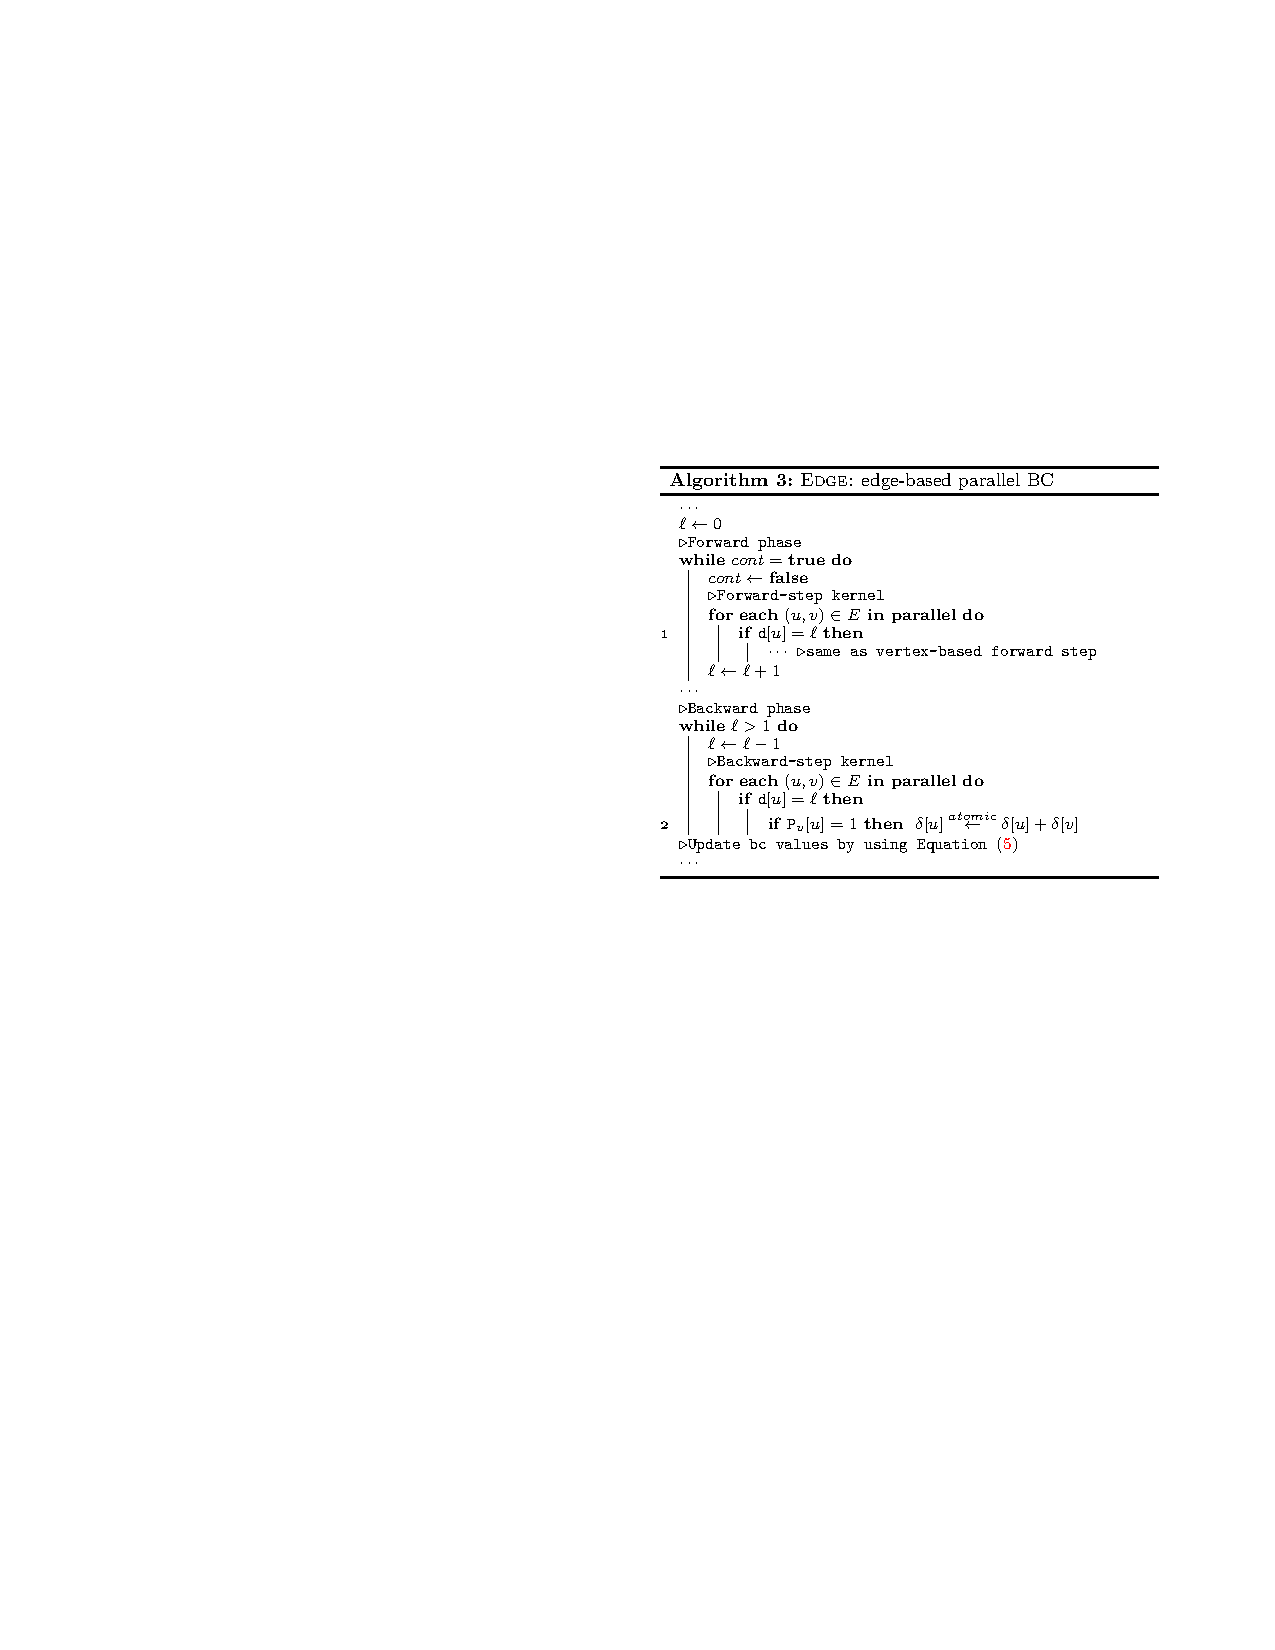
\includegraphics[width=\textwidth, height=0.8\textheight, keepaspectratio]{imgs/gpu-algo-edge}
      \end{figure}
    \end{column}
  \end{columns}

\end{frame}


\begin{frame}
  \frametitle{Vertex virtualization}

  \begin{columns}[onlytextwidth]
    \begin{column}{0.5\textwidth}
      \begin{itemize}
        \item AKA, edge batching, \\ hybrid between vertex- and edge-based
        \item Split high degree vertices into virtual ones with maximum degree $mdeg$
        \item Equivalently, pack up to $mdeg$ edges belonging to the same vertex together
        \item Very small $mdeg = 4$
        \item Need additional auxiliary maps
      \end{itemize}
    \end{column}

    \begin{column}{0.5\textwidth}
      \begin{figure}[t]
        \centering
        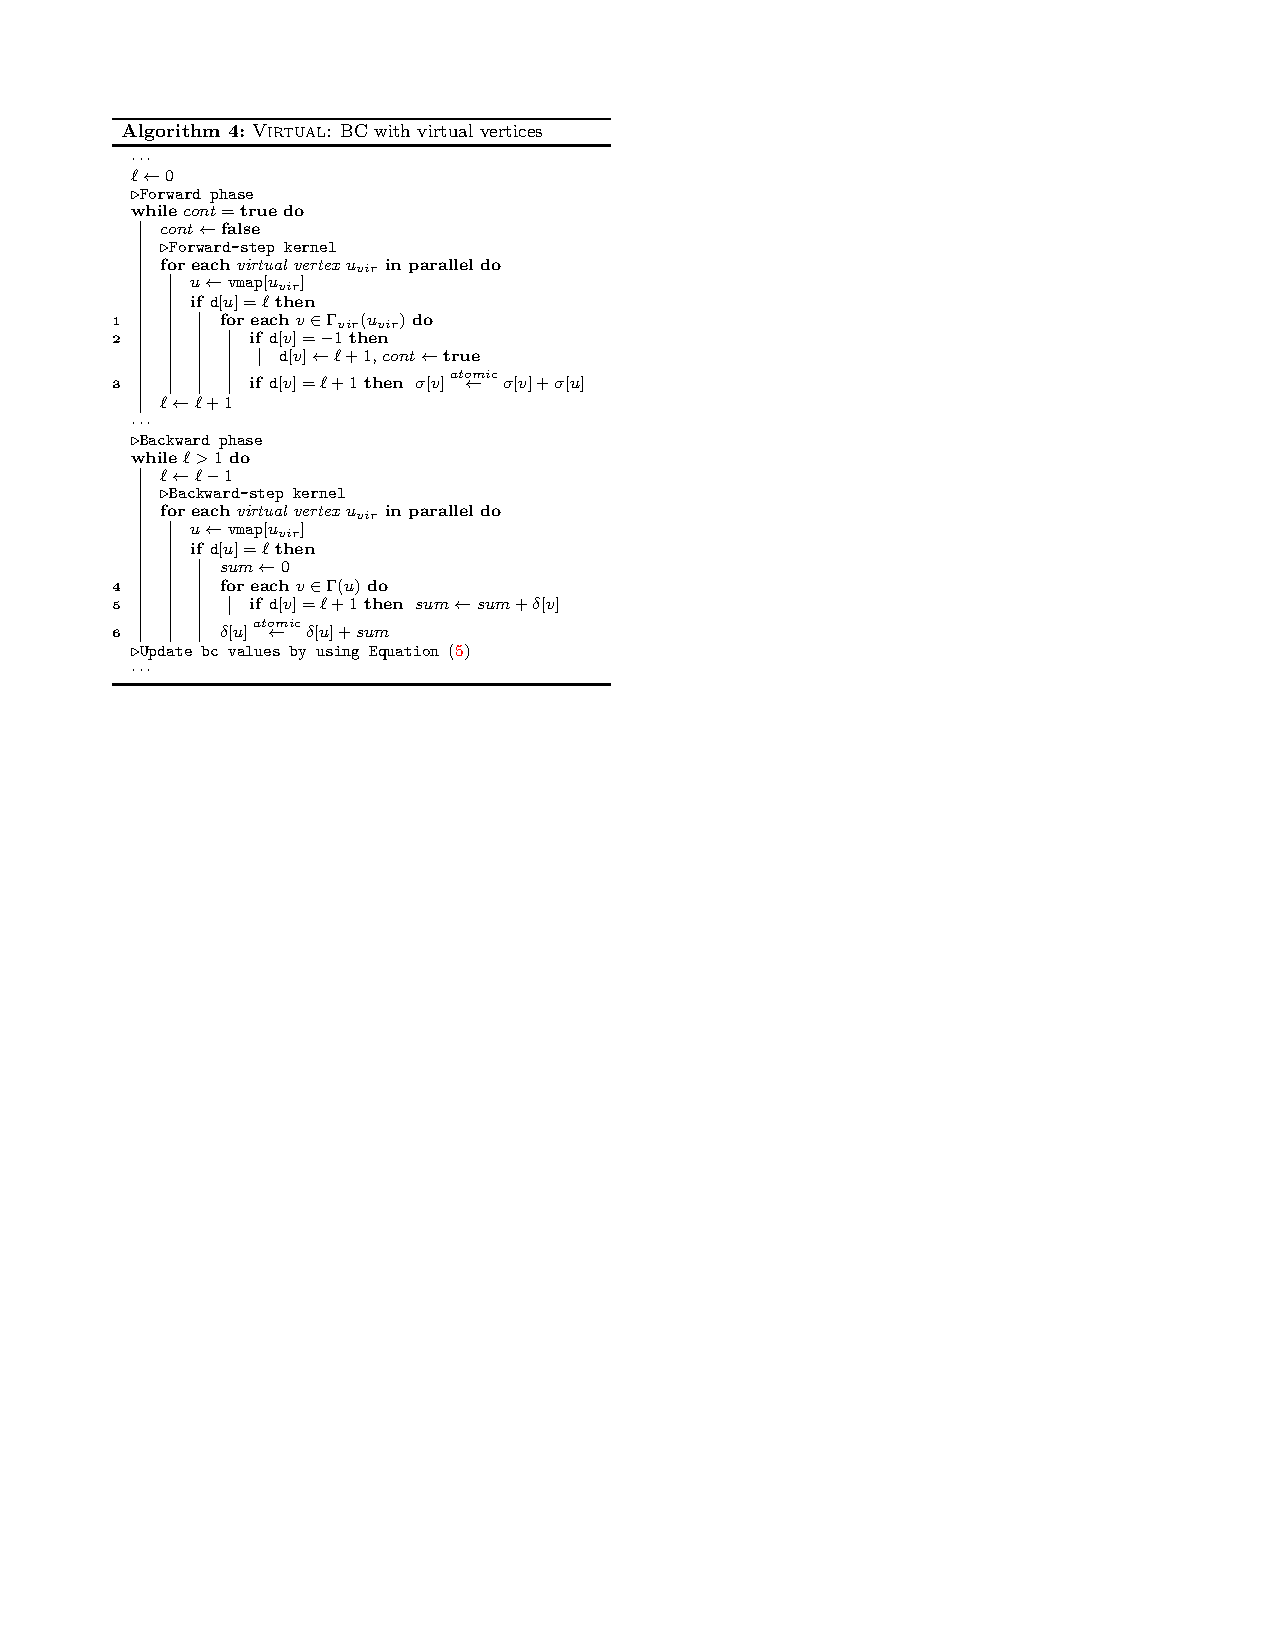
\includegraphics[width=\textwidth, height=0.8\textheight, keepaspectratio]{imgs/gpu-algo-hybrid}
      \end{figure}
    \end{column}
  \end{columns}

\end{frame}


\begin{frame}
  \frametitle{Benefits}

  \begin{itemize}
    \item Compared to vertex-based:
      \begin{itemize}
        \item Reduce load imbalance
      \end{itemize}
    \item Compared to edge-based:
      \begin{itemize}
        \item Reduce number of atomic operations
        \item Reduce memory footprint
      \end{itemize}
    \item Predecessors stored implicitly in the \spdag level (reduced memory usage)
    \item Memory layout can be further optimized to coalesce latency via \emph{striding}:
      \begin{itemize}
        \item Distribute edges to virtual vertices in round-robin
        \item When accessed in parallel, they create faster sequential memory access pattern
      \end{itemize}
  \end{itemize}
\end{frame}


\begin{frame}
  \frametitle{Results}

  \begin{figure}[t]
    \centering
    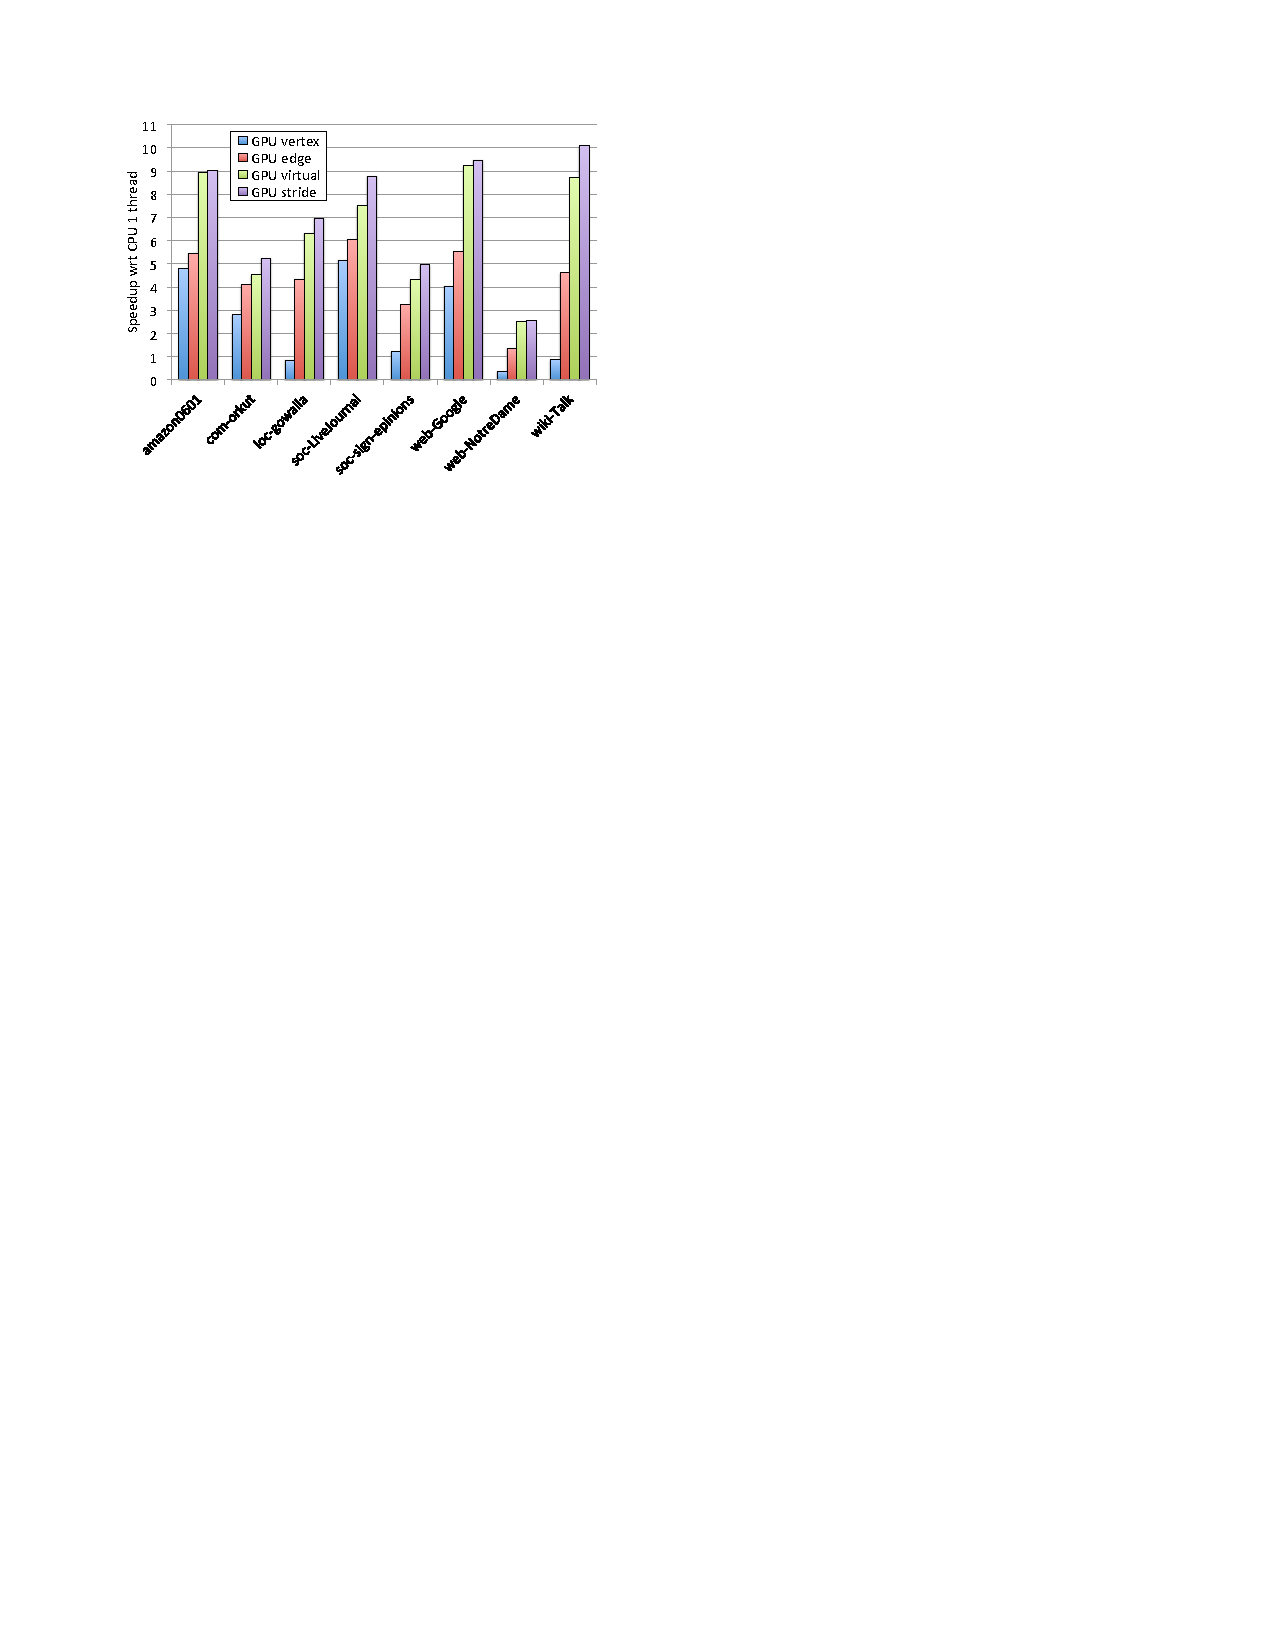
\includegraphics[width=\textwidth, height=0.6\textheight, keepaspectratio]{imgs/gpu-results1}
    \caption{Speedup over Brandes' on CPU on real graphs with 32-core GPU ($s= 1k, \ldots, 100k$)}
  \end{figure}

  \begin{itemize}
    \item Results computed only on a sample of sources and extrapolated linearly
  \end{itemize}
\end{frame}


%\begin{frame}
%  \frametitle{Results}
%
%  \begin{figure}[t]
%    \centering
%    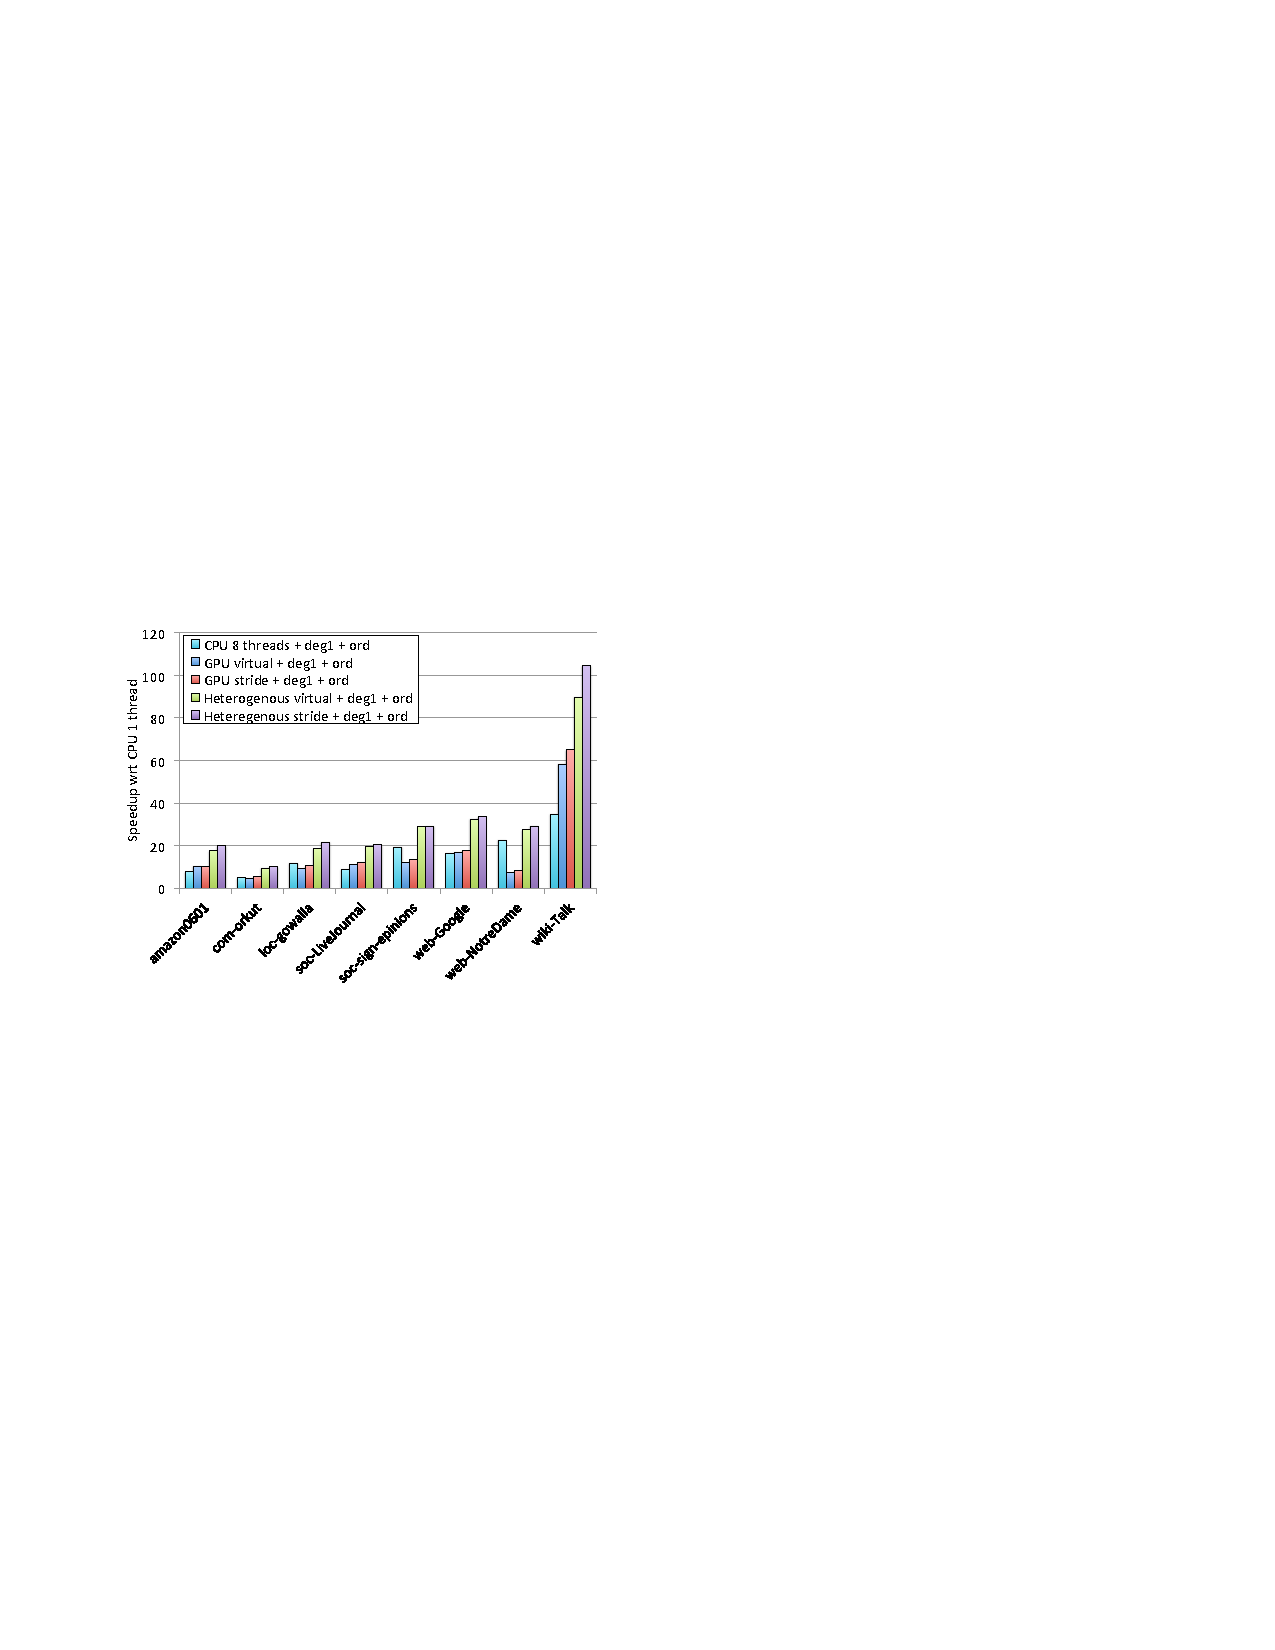
\includegraphics[width=\textwidth, height=0.6\textheight, keepaspectratio]{imgs/gpu-results2}
%    \caption{Speedup over Brandes' on CPU on real graphs with 32-core GPU}
%  \end{figure}
%
%\end{frame}



\subsection{Exact Algorithms for Dynamic Graphs}

%% Green et al.
\begin{frame}
  \centering
  \vfill
  {\huge A Fast Algorithm for Streaming Betweenness Centrality}
  \vfill
  {\Large O. Green, R. McColl, D. A. Bader}
  \vfill
  {\large SocialCom '12: International Conference on Social Computing}
  \vfill
\end{frame}


\begin{frame}
  \frametitle{Intuition}

  \begin{itemize}
    \item Make Brandes' algorithm incremental
    \item Keep additional data structures to avoid recomputing partial results
      \begin{itemize}
        \item Rooted \spdag for each source $s \in V$
        \item Depth in the tree for $t$ = distance of $t$ from $s$
      \end{itemize}
    \item Re-run parts of modified Brandes' algorithm on edge update
    \item Support only edge addition (on unweighted graphs)
  \end{itemize}

\end{frame}


\begin{frame}
  \frametitle{Data structures}

  \begin{itemize}
    \item One $\spdag_s$ for each source $s \in V$, which contains for each other vertex $t \in V$:
      \begin{itemize}
        \item Distance $\dist_{st}$, paths $\paths_{st}$, dependencies $\dep_{s}(t)$, predecessors $\pred_{s}(t)$
        \item Additional per-level queues for exploration
      \end{itemize}
  \end{itemize}
  \begin{itemize}
    \item On addition of edge $(u,v)$, let $dd = |d_{su} - d_{sv}|$:
      \begin{itemize}
        \item $dd = 0$ same~level
        \item $dd = 1$ adjacent~level
        \item $dd > 1$ non-adjacent~level
      \end{itemize}
  \end{itemize}

\end{frame}


\begin{frame}
  \frametitle{Same level addition}
  \begin{columns}[onlytextwidth]

    \begin{column}{0.5\textwidth}
      \begin{itemize}
        \item $dd = 0$
        \item Edge creates no new shortest paths
        \item No change to betweenness \\ due to this source
      \end{itemize}
    \end{column}

    \begin{column}{0.5\textwidth}
      \begin{figure}[t]
        \centering
        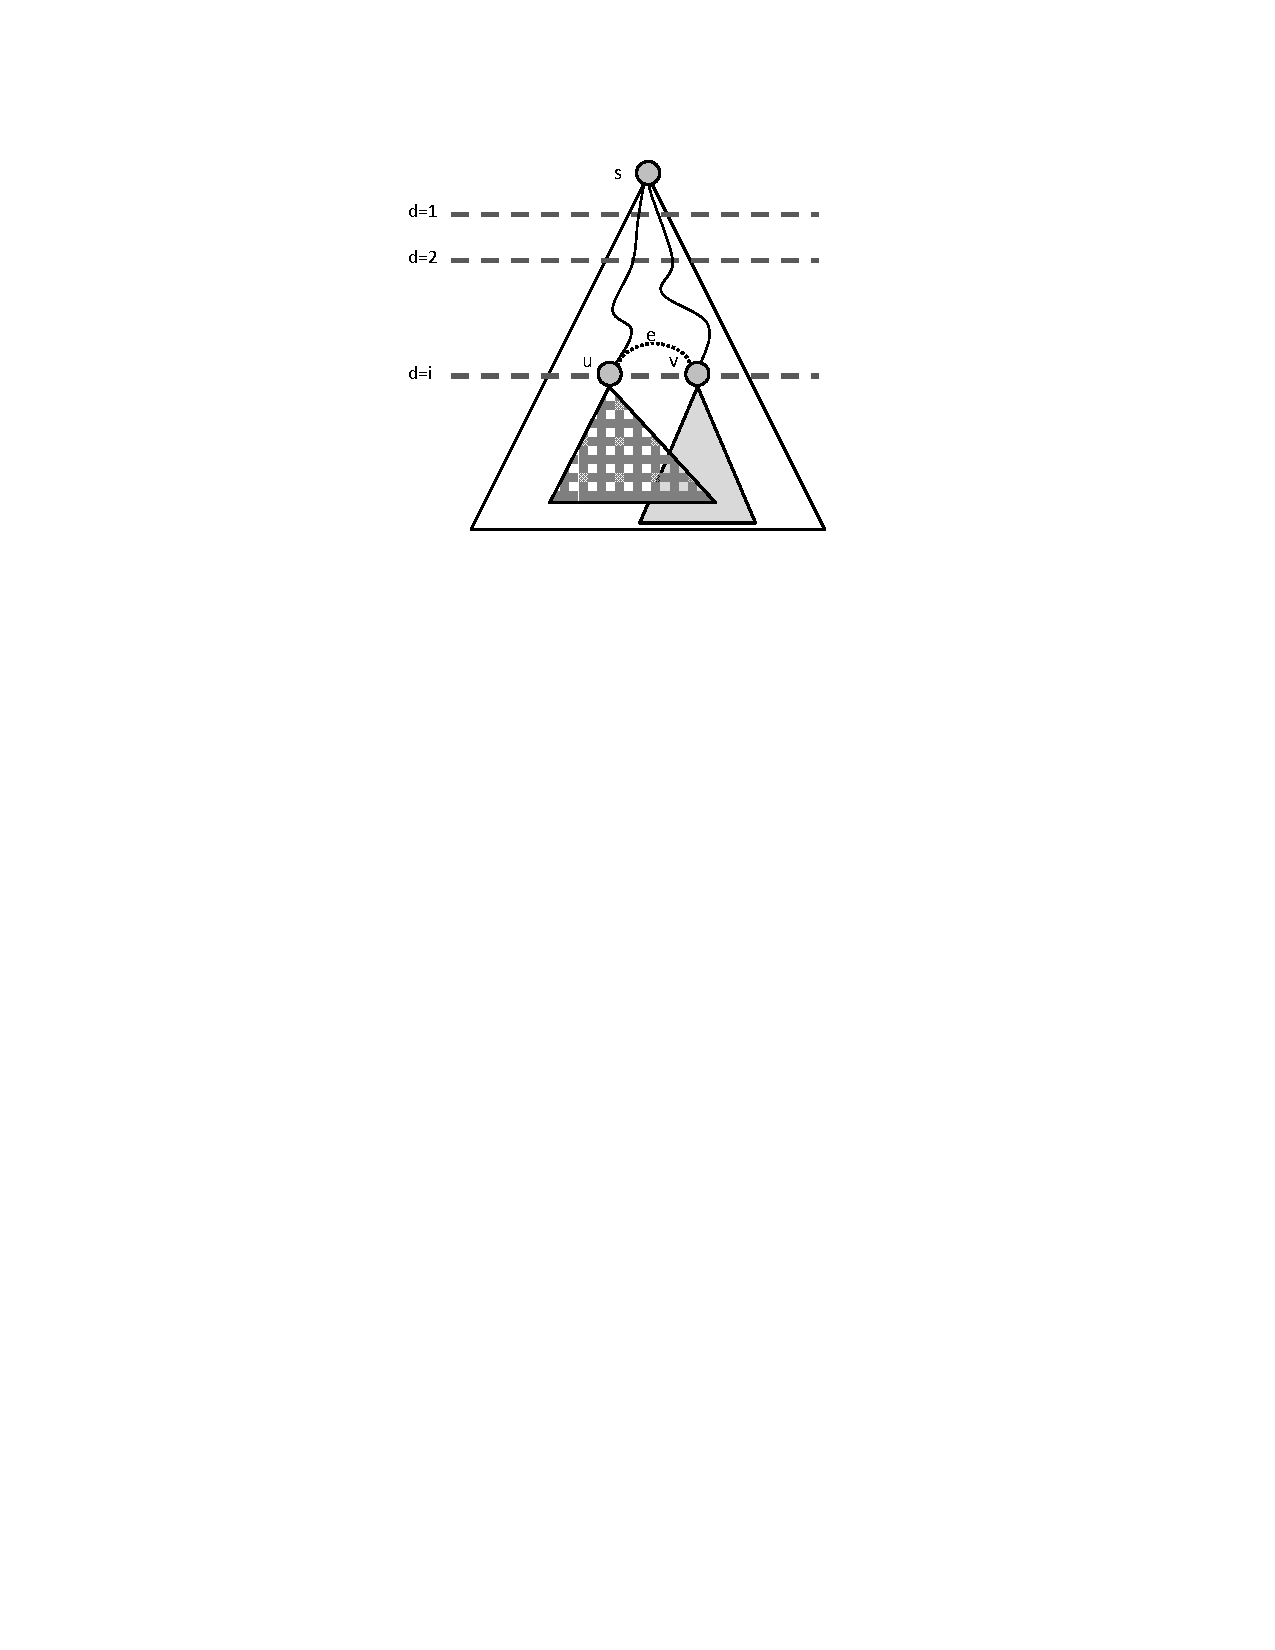
\includegraphics[width=\textwidth, height=\textheight, keepaspectratio]{imgs/green-0lvl-compressed}
      \end{figure}
    \end{column}
  \end{columns}

\end{frame}


\begin{frame}
  \frametitle{Adjacent level addition}
  \begin{columns}[onlytextwidth]

    \begin{column}{0.5\textwidth}
      \begin{itemize}
        \item $dd = 1$
        \item Let $u_{high} = u ,\, u_{low} = v$
        \item Edge creates new shortest paths
        \item \spdag unchanged
        \item Changes in \paths confined to sub-dag rooted in $u_{low}$
        \item Changes in \dep also spread above to decrease old dependency and account for new dependency
        \item Example: $w$ and predecessors have now only $\sfrac{1}{2}$ of dependency on sub-dag rooted in $u_{low}$
      \end{itemize}
    \end{column}

    \begin{column}{0.5\textwidth}
      \begin{figure}[t]
        \centering
        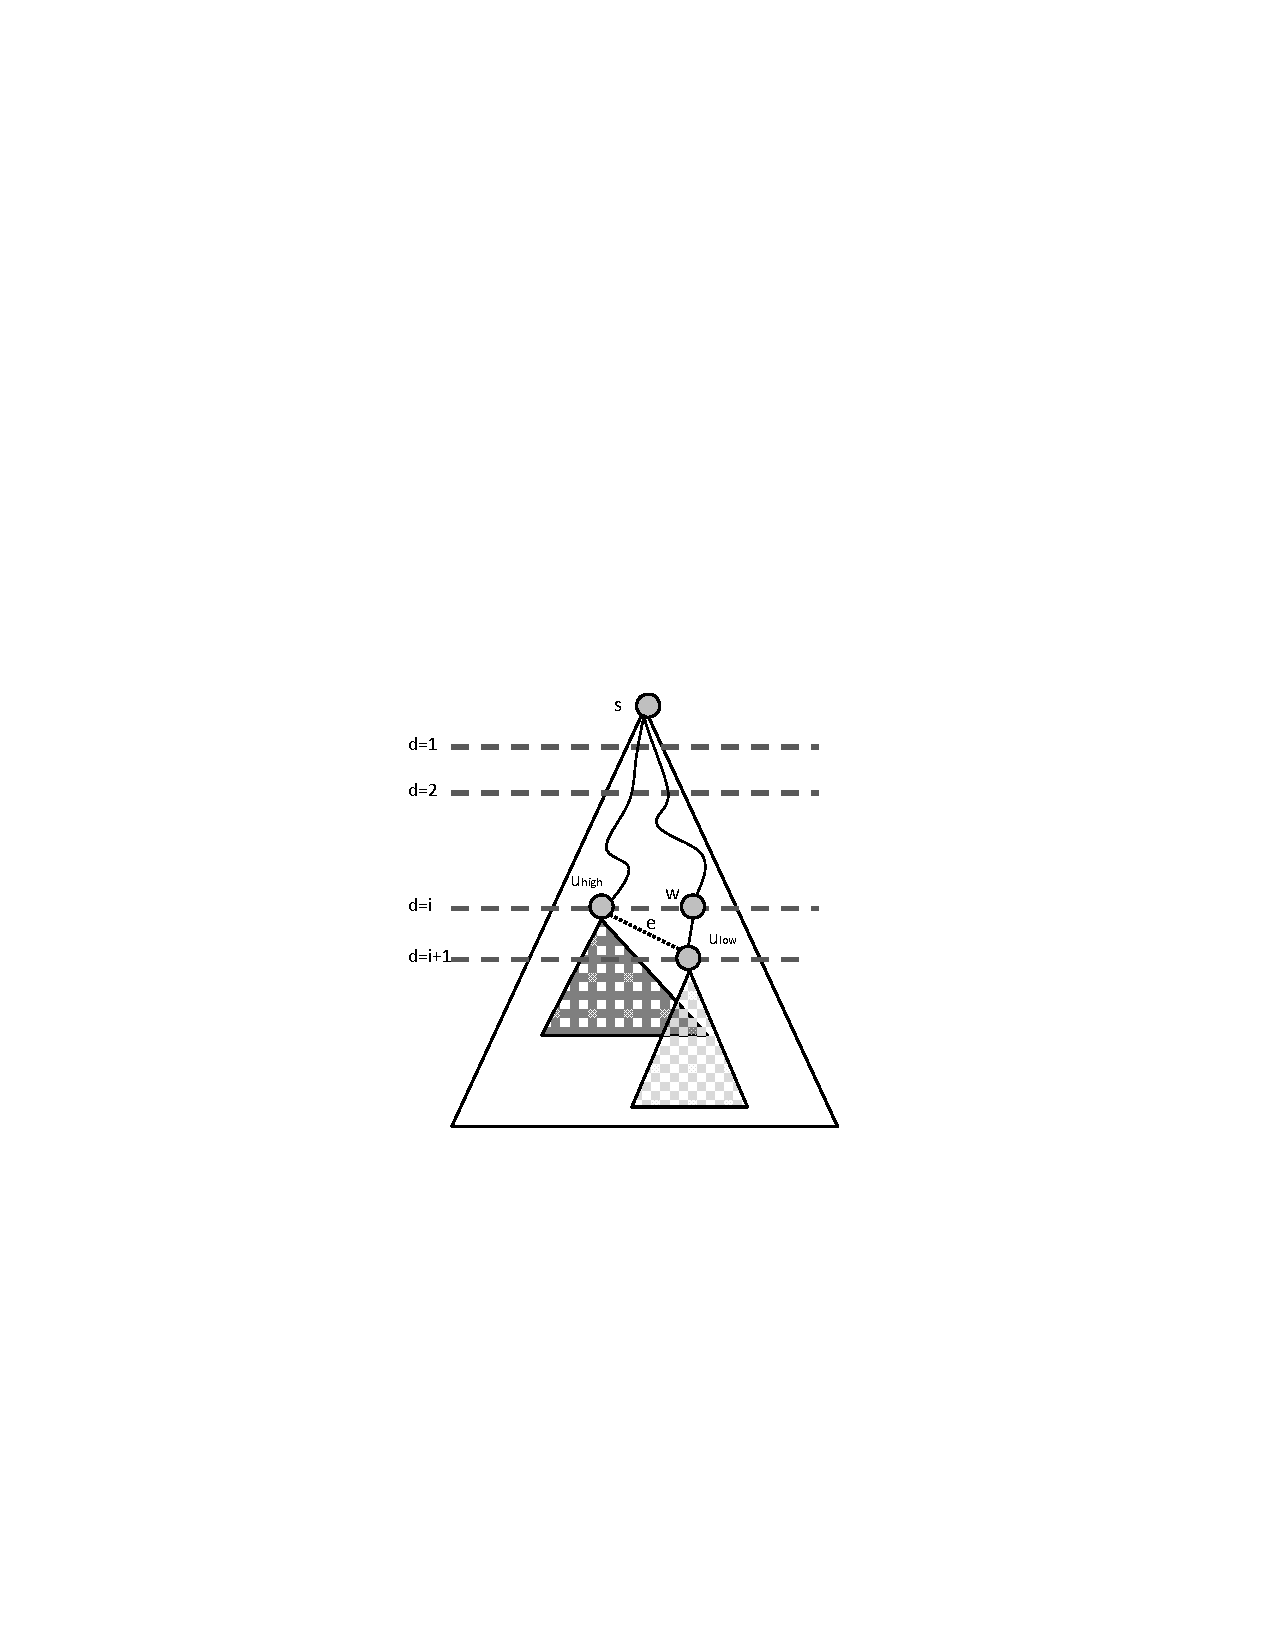
\includegraphics[width=\textwidth, height=\textheight, keepaspectratio]{imgs/green-1lvl-compressed}
      \end{figure}
    \end{column}
  \end{columns}

\end{frame}


\begin{frame}
  \frametitle{Algorithm}
  \begin{columns}[onlytextwidth]

    \begin{column}{0.5\textwidth}
      \begin{itemize}
        \item During exploration:
          \begin{itemize}
            \item Fix \paths
            \item Mark visited vertices
            \item Enqueue for further processing
          \end{itemize}
      \end{itemize}
    \end{column}
    \begin{column}{0.5\textwidth}
      \begin{itemize}
        \item During backtracking:%
          \begin{itemize}
            \item Fix \dep and \betw
            \item Recurse up the whole \spdag
          \end{itemize}
      \end{itemize}
    \end{column}
  \end{columns}
      \begin{figure}[t]
        \centering
        %        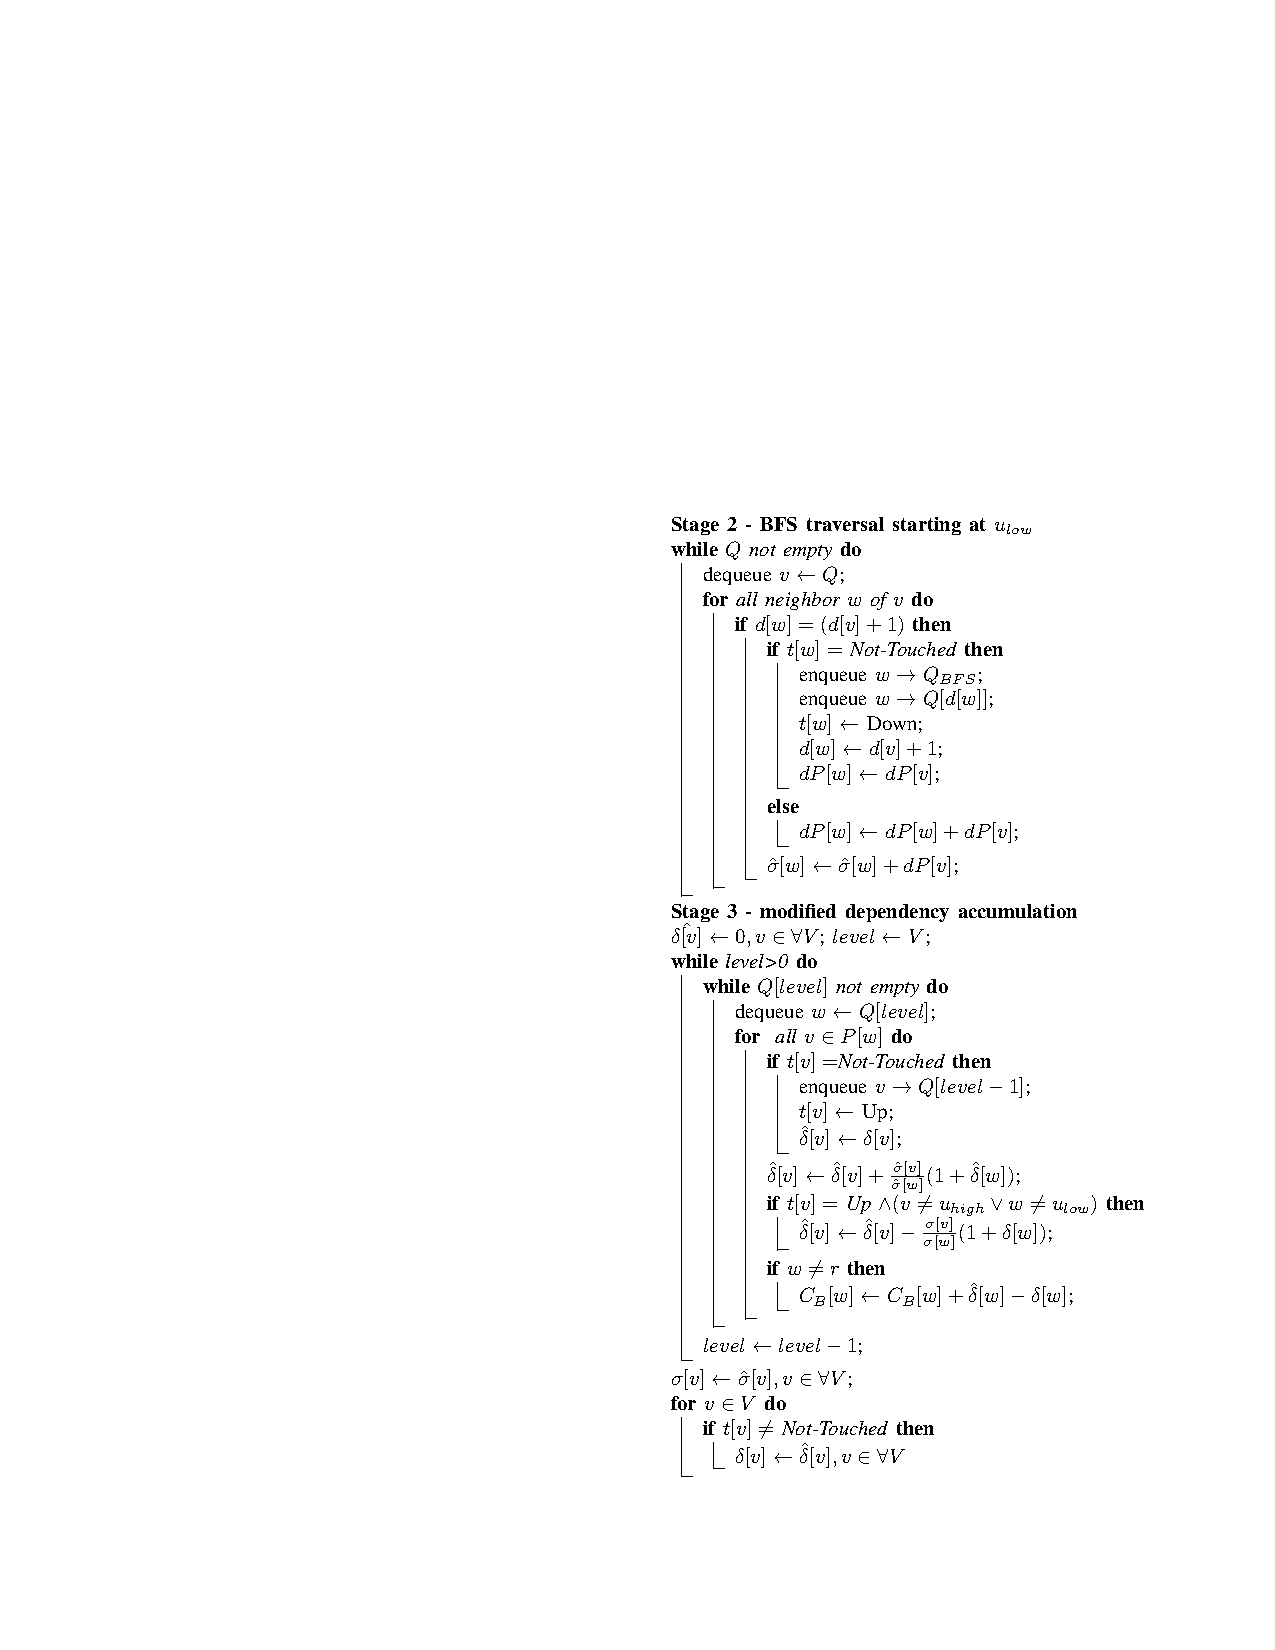
\includegraphics[width=\textwidth, height=0.8\textheight, keepaspectratio]{imgs/green-algo}
        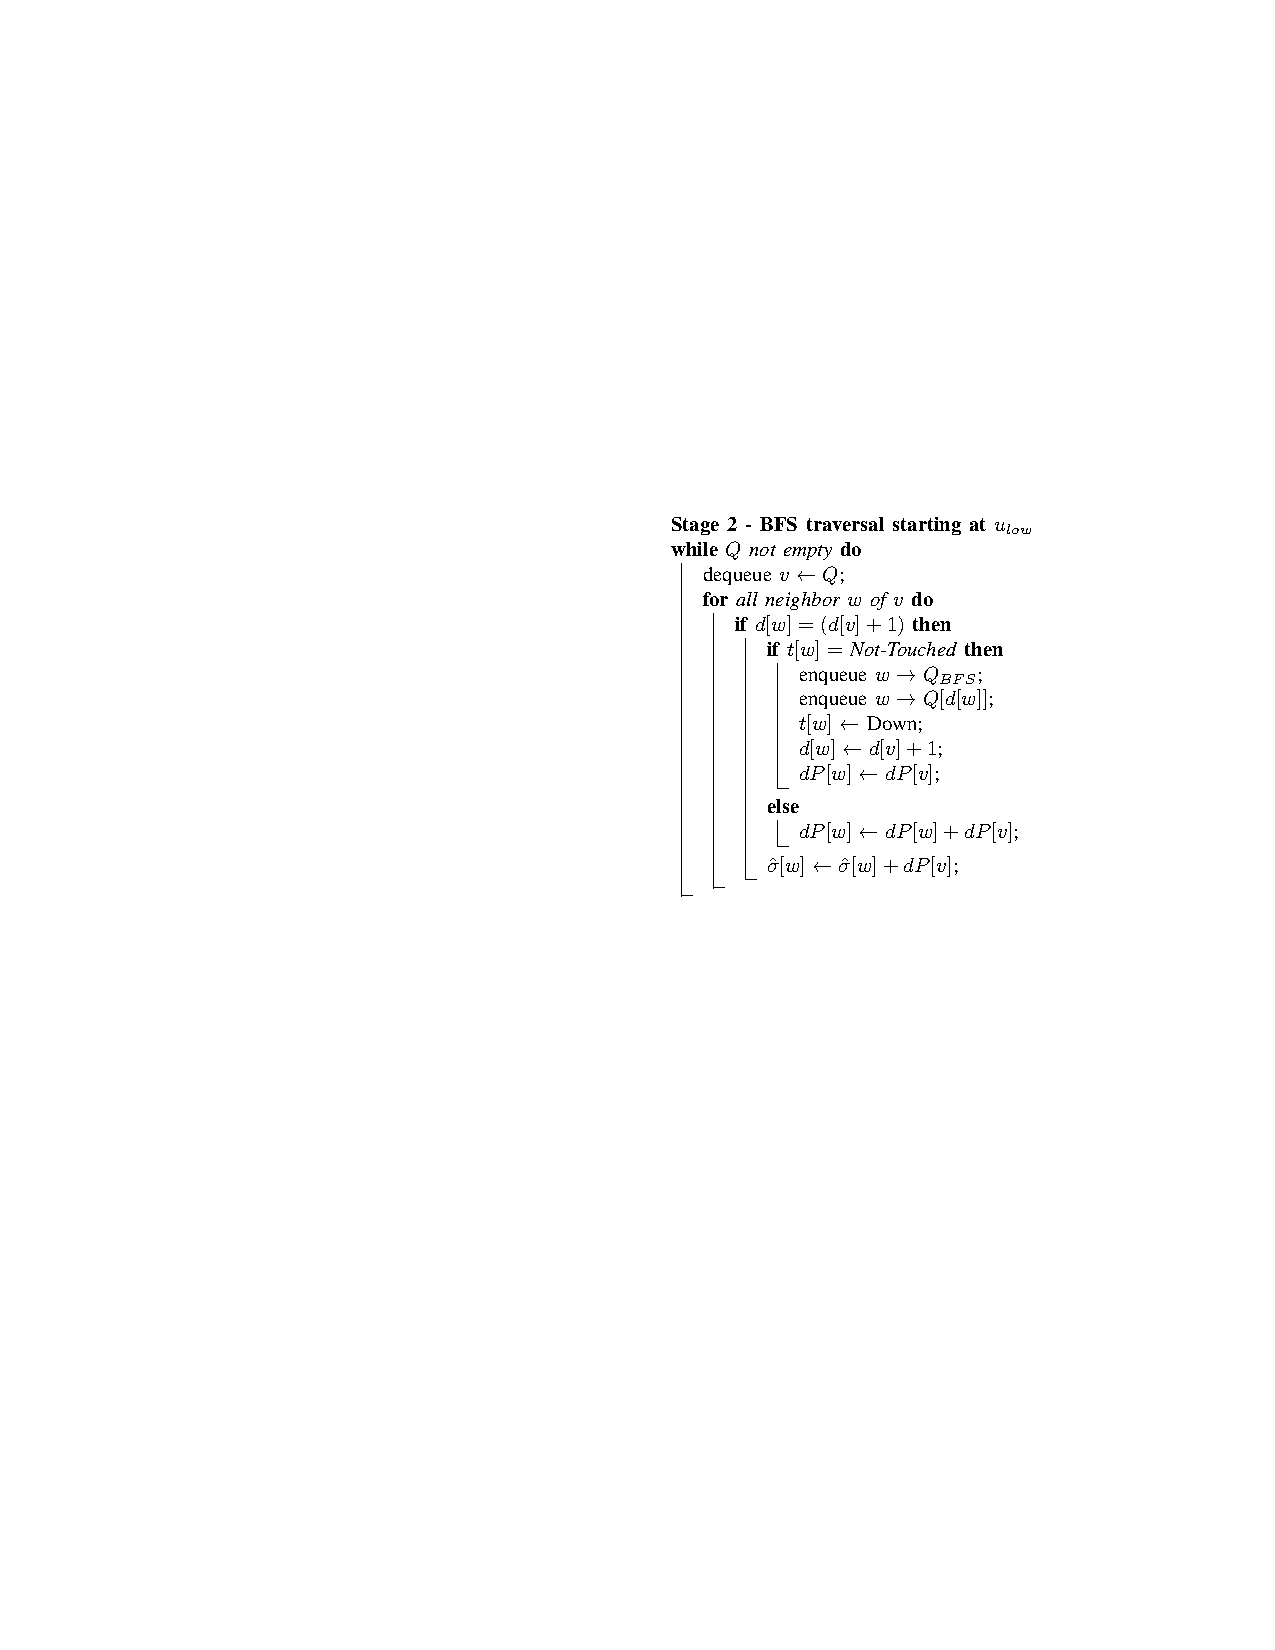
\includegraphics[width=0.45\textwidth, height=0.6\textheight, keepaspectratio, valign=t]{imgs/green-algo1}
        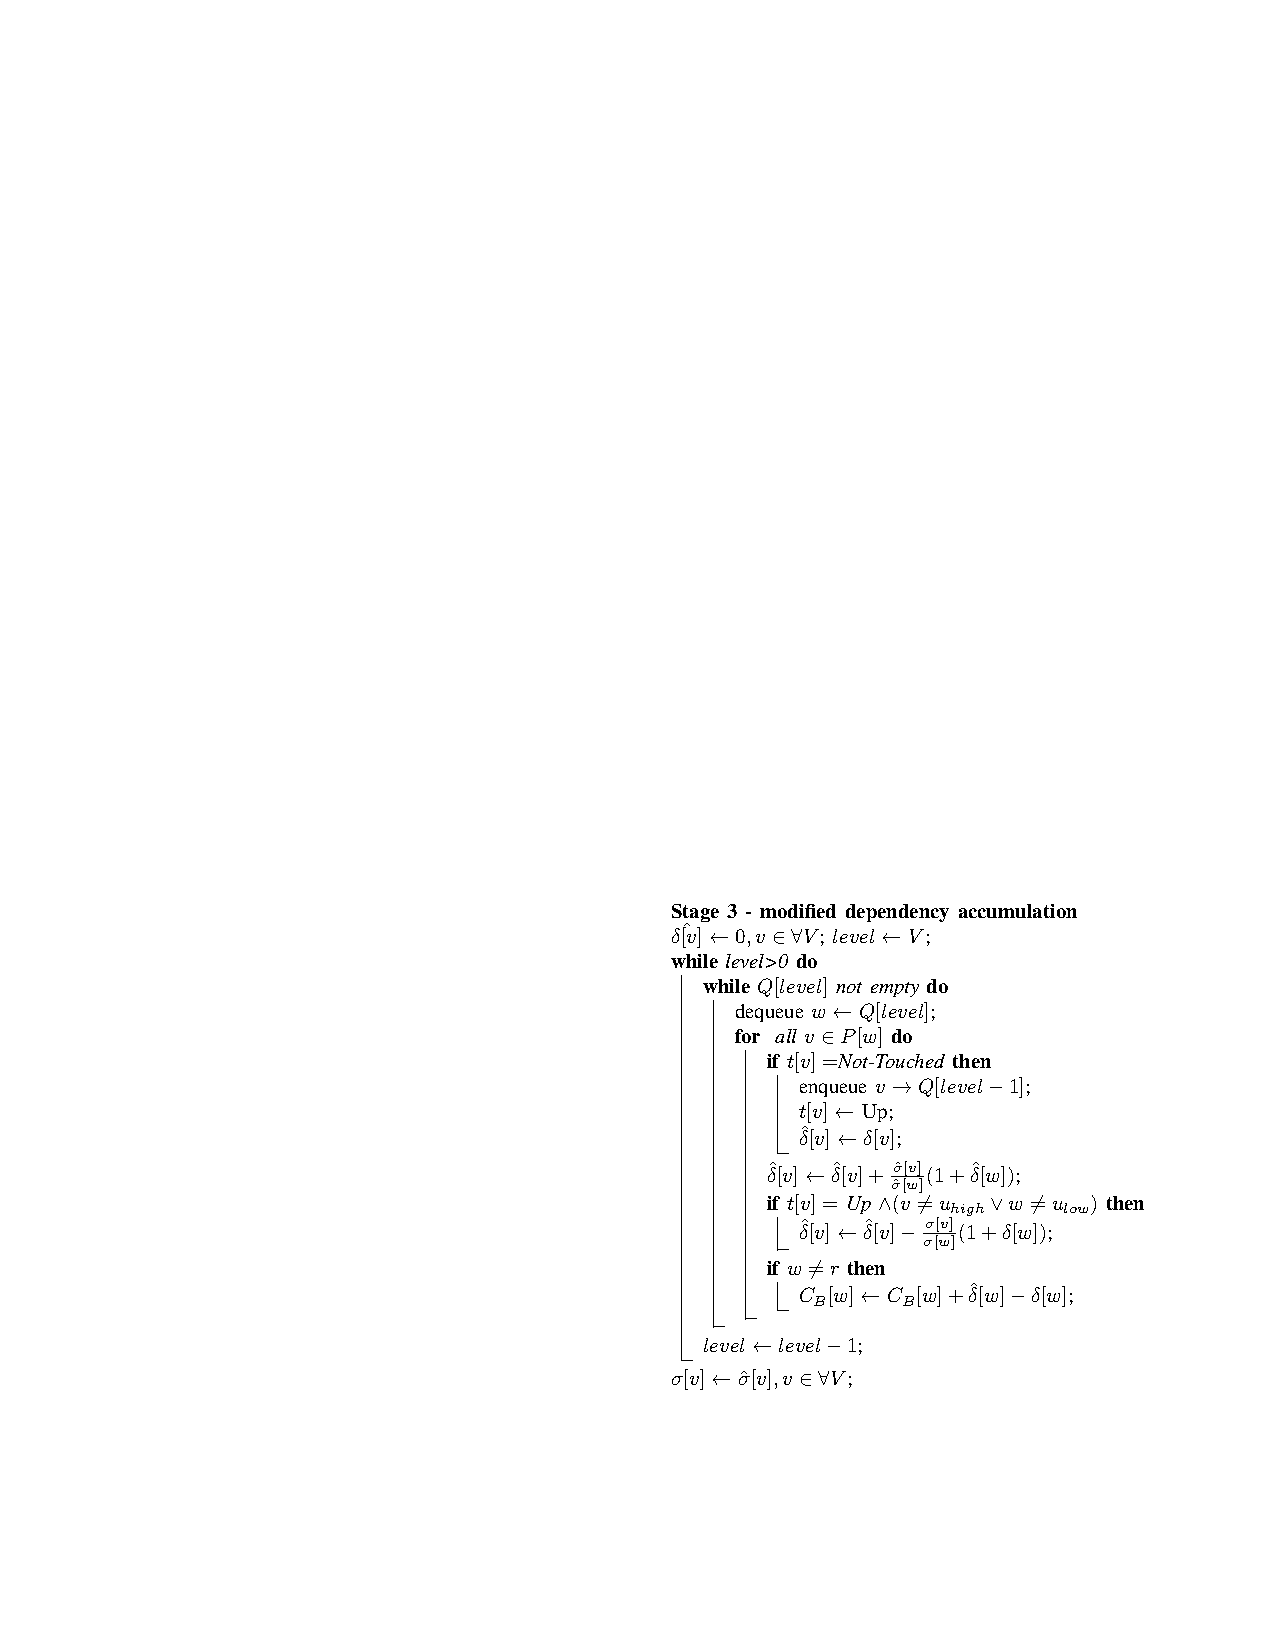
\includegraphics[width=0.6\textwidth, height=0.6\textheight, keepaspectratio, valign=t]{imgs/green-algo2}
      \end{figure}
\end{frame}


\begin{frame}
  \frametitle{Non-adjacent level addition}

  \begin{columns}[onlytextwidth]

    \begin{column}{0.5\textwidth}
      \begin{itemize}
        \item $dd > 1$
        \item Edge creates new shortest paths
        \item Changes to \spdag (new distances)
        \item Algorithm only sketched \\ (most details missing)
      \end{itemize}
    \end{column}

    \begin{column}{0.5\textwidth}
      \begin{figure}[t]
        \centering
        \includegraphics<1>[width=\textwidth, height=0.8\textheight, keepaspectratio]{imgs/green-2lvl-before-compressed}
        \includegraphics<2>[width=\textwidth, height=0.8\textheight, keepaspectratio]{imgs/green-2lvl-after-compressed}
      \end{figure}
    \end{column}
  \end{columns}

\end{frame}


\begin{frame}
  \frametitle{Complexity}

  \begin{itemize}
    \item Time: $O(n^2 + nm)$ $\leftarrow$ same as Brandes'
    \item In practice, algorithm is much faster
  \end{itemize}
  \begin{itemize}
    \item Space: $O(n^2 + nm)$ $\leftarrow$ higher than Brandes'
    \item For each source, a \spdag of complexity $n + m$
  \end{itemize}

\end{frame}


\begin{frame}
  \frametitle{Results}

  \begin{figure}[t]
    \centering
    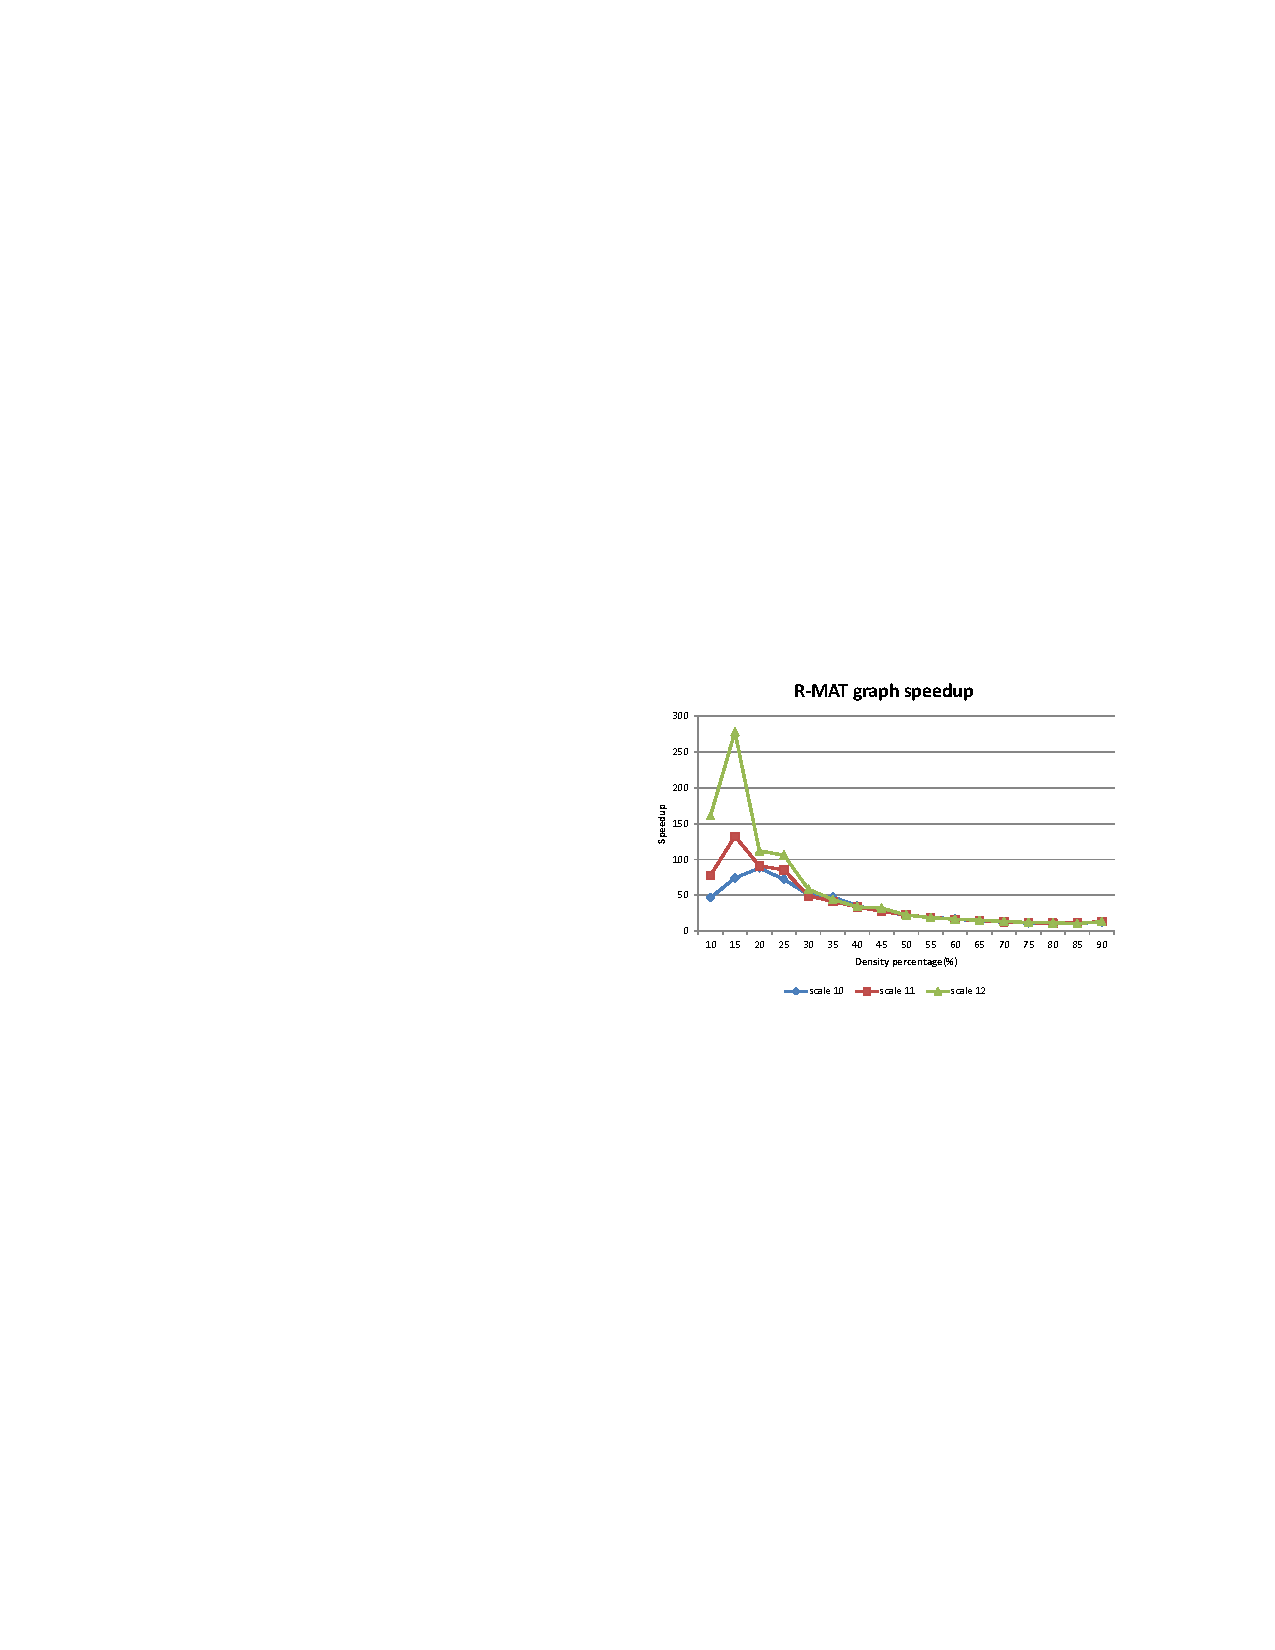
\includegraphics[width=\textwidth, height=0.7\textheight, keepaspectratio]{imgs/green-results1}
    \caption{Speedup over Brandes' on synthetic graphs ($n = 4096$)}
  \end{figure}

\end{frame}


\begin{frame}
  \frametitle{Conclusions}

  \begin{itemize}
    \item Up to 2 orders of magnitude speedup
    \item Super-quadratic space bottleneck
  \end{itemize}

\end{frame}


%% QUBE
\begin{frame}
  \centering
  \vfill
  {\huge QUBE: a Quick algorithm for Updating BEtweenness centrality}
  \vfill
  {\Large M. Lee, J. Lee, J. Park, R. Choi, C. Chung}
  \vfill
  {\large WWW '12: International World Wide Web Conference}
  \vfill
\end{frame}

\begin{frame}
  \frametitle{Intuition}

  \begin{itemize}
    \item No need to update all vertices when a new edge is added
    \item Prune vertices whose \betw does not change
    \item Large reduction in all-pairs shortest paths to be re-computed
    \item Support both edge additions and removals
  \end{itemize}
\end{frame}


\begin{frame}
  \frametitle{Minimum Cycle Basis}

  \begin{itemize}
    \item $G=(V,E)$ undirected graph
    \item \emph{Cycle} $C \subseteq E$ s.t. $\forall v \in V$, $v$ incident to even number of edges in $C$
    \item Represented as edge incidence vector $\nu \in \{ 0,1 \}^{|E|}$, where $\nu(e) = 1 \iff e \in C$
    \item \emph{Cycle Basis} = set of linearly independent cycles
    \item \emph{Minimum Cycle Basis} = on weighted graph with non-negative weights $w_e$, cycle basis of minimum total weight $w(C) = \sum_{i} w(C_i)$ where $w(C_i) = \sum_{e \in C_i} w_e$
  \end{itemize}
\end{frame}


\begin{frame}
  \frametitle{Minimum Cycle Basis Example}
  \begin{itemize}
    \item Three cycle basis sets: $\{C_1, C_2\} , \{C_1, C_3\} , \{C_2, C_3\}$
    \item If all edges have same weight $w_e = 1$, $MCB = \{C_1, C_2\}$
  \end{itemize}
  \begin{figure}[H]
    \centering
    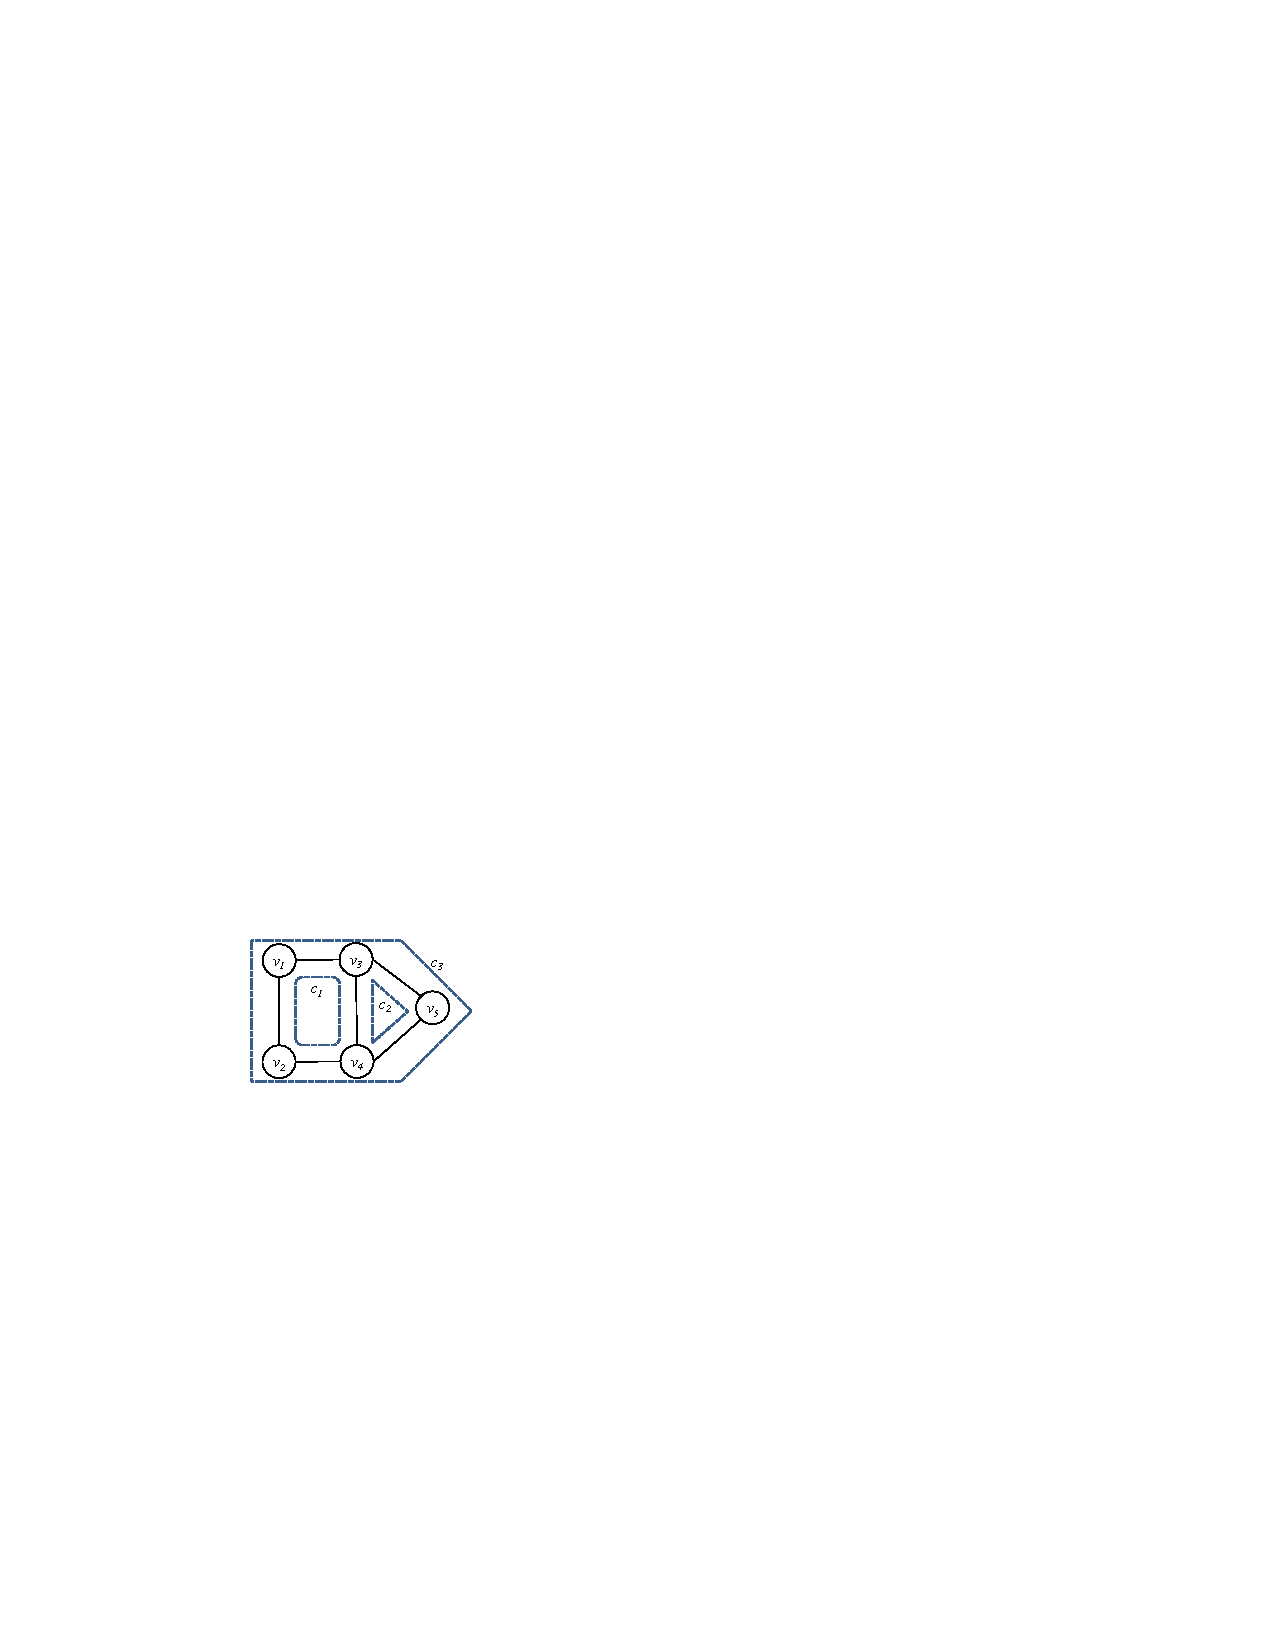
\includegraphics[scale=2]{imgs/qube-mcb}
  \end{figure}
\end{frame}


\begin{frame}
  \frametitle{Minimum Union Cycle}

  \begin{itemize}
    \item Given a MCB $C$ and minimum cycles $C_i \in C$
    \item Let $V_{C_i}$ be the set of vertices induced by $C_i$
    \item Recursively union two $V_{C_i}$ if they share at least one vertex
    \item The final set of vertices is a \emph{Minimum Union Cycle} $MUC$
  \end{itemize}

  \begin{itemize}
    \item $MUC$s are disjoint sets of vertices
    \item $MUC(v)$ = the $MUC$ which contains vertex $v$
  \end{itemize}
\end{frame}


\begin{frame}
  \frametitle{Connection Vertex}

  \begin{itemize}
    \item \emph{Articulation Vertex} = vertex $v$ whose deletion makes the graph disconnected
    \item Biconnected graph = graph with no articulation vertex
    \item Vertex $v$ is an articulation vertex $\iff$ v belongs to two biconnected components
  \end{itemize}

  \begin{itemize}
    \item \emph{Connection Vertex} = vertex $v$ that
      \begin{itemize}
        \item is an articulation vertex
        \item has an edge to vertex $w \not\in MUC(v)$
      \end{itemize}
  \end{itemize}
\end{frame}


\begin{frame}
  \frametitle{Connection Vertex Example}

  \begin{columns}[onlytextwidth]
    \begin{column}{0.5\textwidth}
      \begin{itemize}
        \item If $(v_3, v_4)$ is added, $MUC(v_3) = \{ v_1, v_2, v_3, v_4 \}$
        \item $v_1, v_2, v_3$ are connection vertices of $MUC(v_3)$
        \item Let $G_i$ be the disconnected subgraph generated by removing $v_i$
      \end{itemize}
    \end{column}

    \begin{column}{0.5\textwidth}
      \begin{figure}[t]
        \centering
        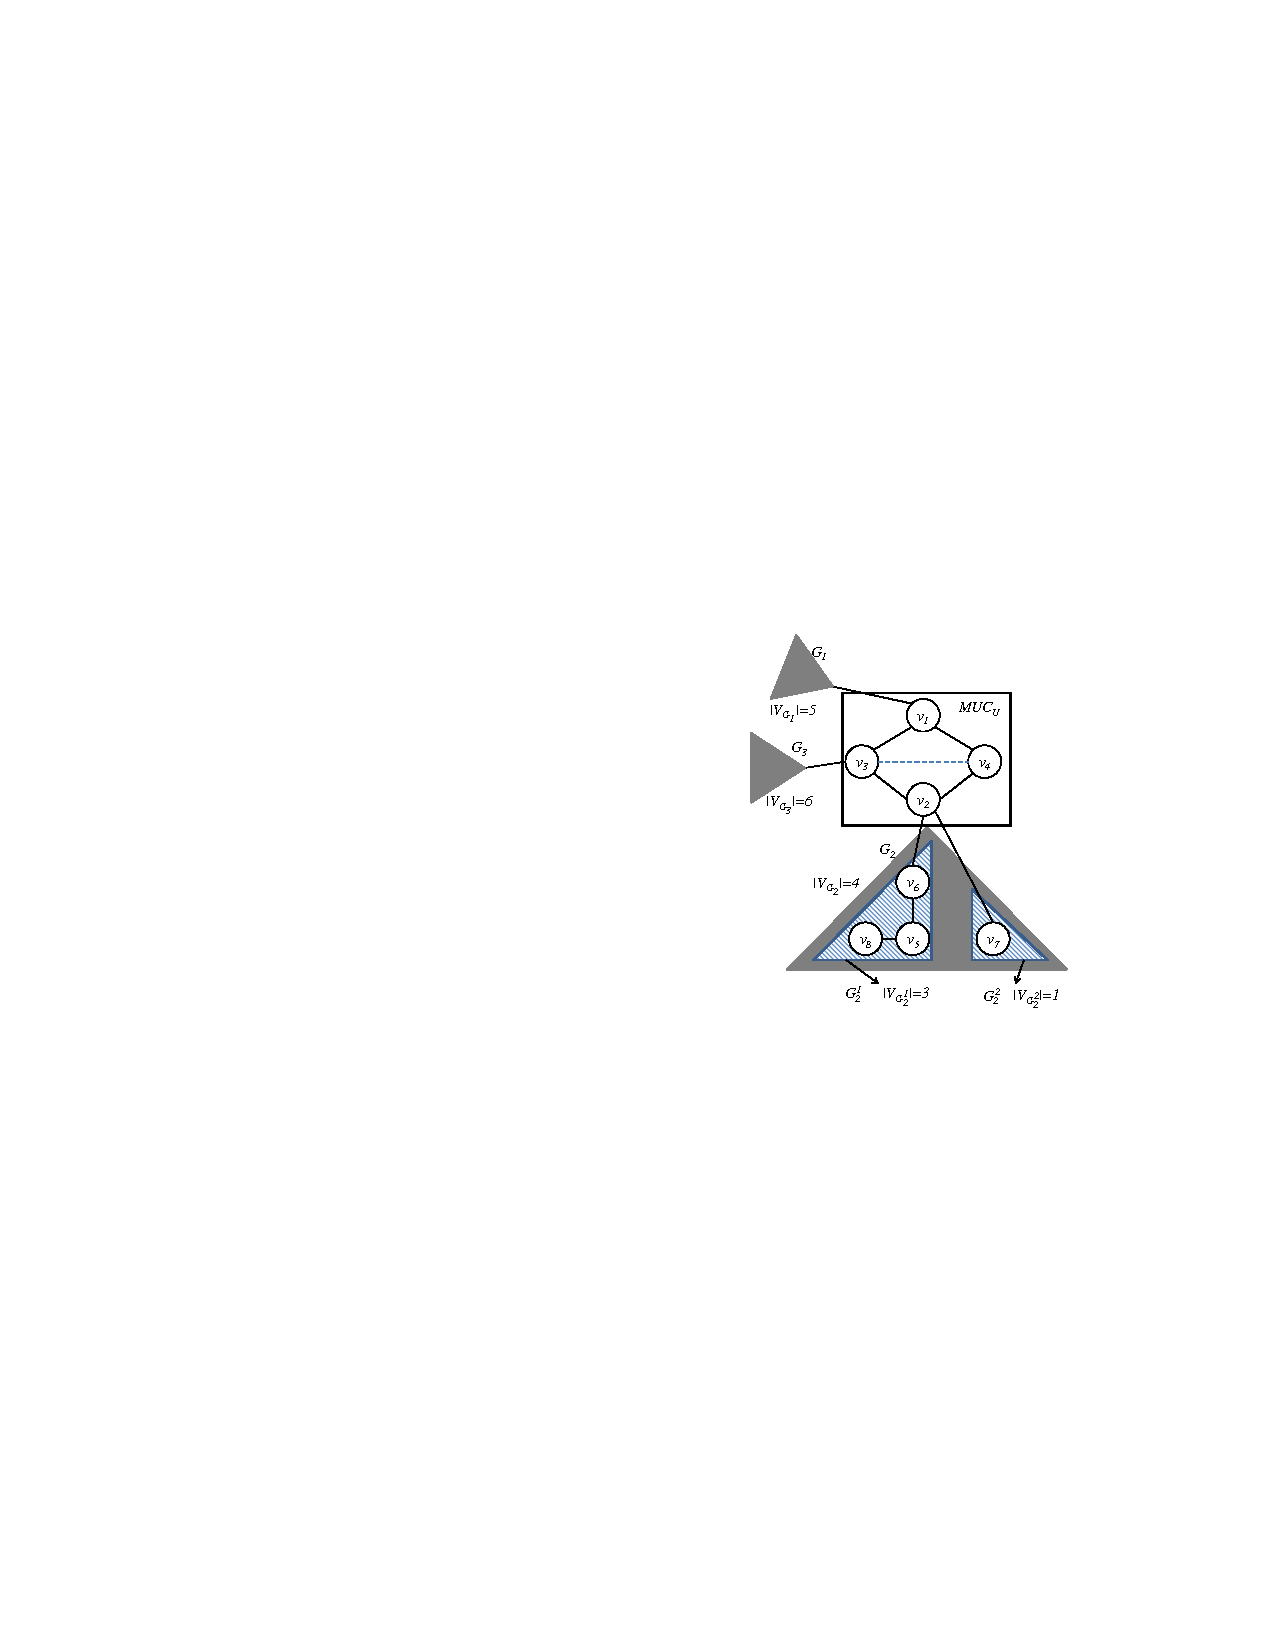
\includegraphics[width=\textwidth, height=0.8\textheight, keepaspectratio]{imgs/qube-biconnected}
      \end{figure}
    \end{column}
  \end{columns}

\end{frame}


\begin{frame}
  \frametitle{Finding MUCs}

  \begin{itemize}
    \item Finding an $MCB$ is well studied
    \item Kavitha, Mehlhorn, Michail, Paluch. ``A faster algorithm for minimum cycle basis of graphs''. ICALP 2004
    \item Finding $MUC$ from $MCB$ relatively straightforward (just union sets of vertices)
    \item Also find connection vertices for each $MUC$
    \item All done as a preprocessing step
    \item Need to be updated at runtime
  \end{itemize}
\end{frame}


\begin{frame}
  \frametitle{Updating MUCs -- Addition}

  \begin{figure}[t]
    \centering
    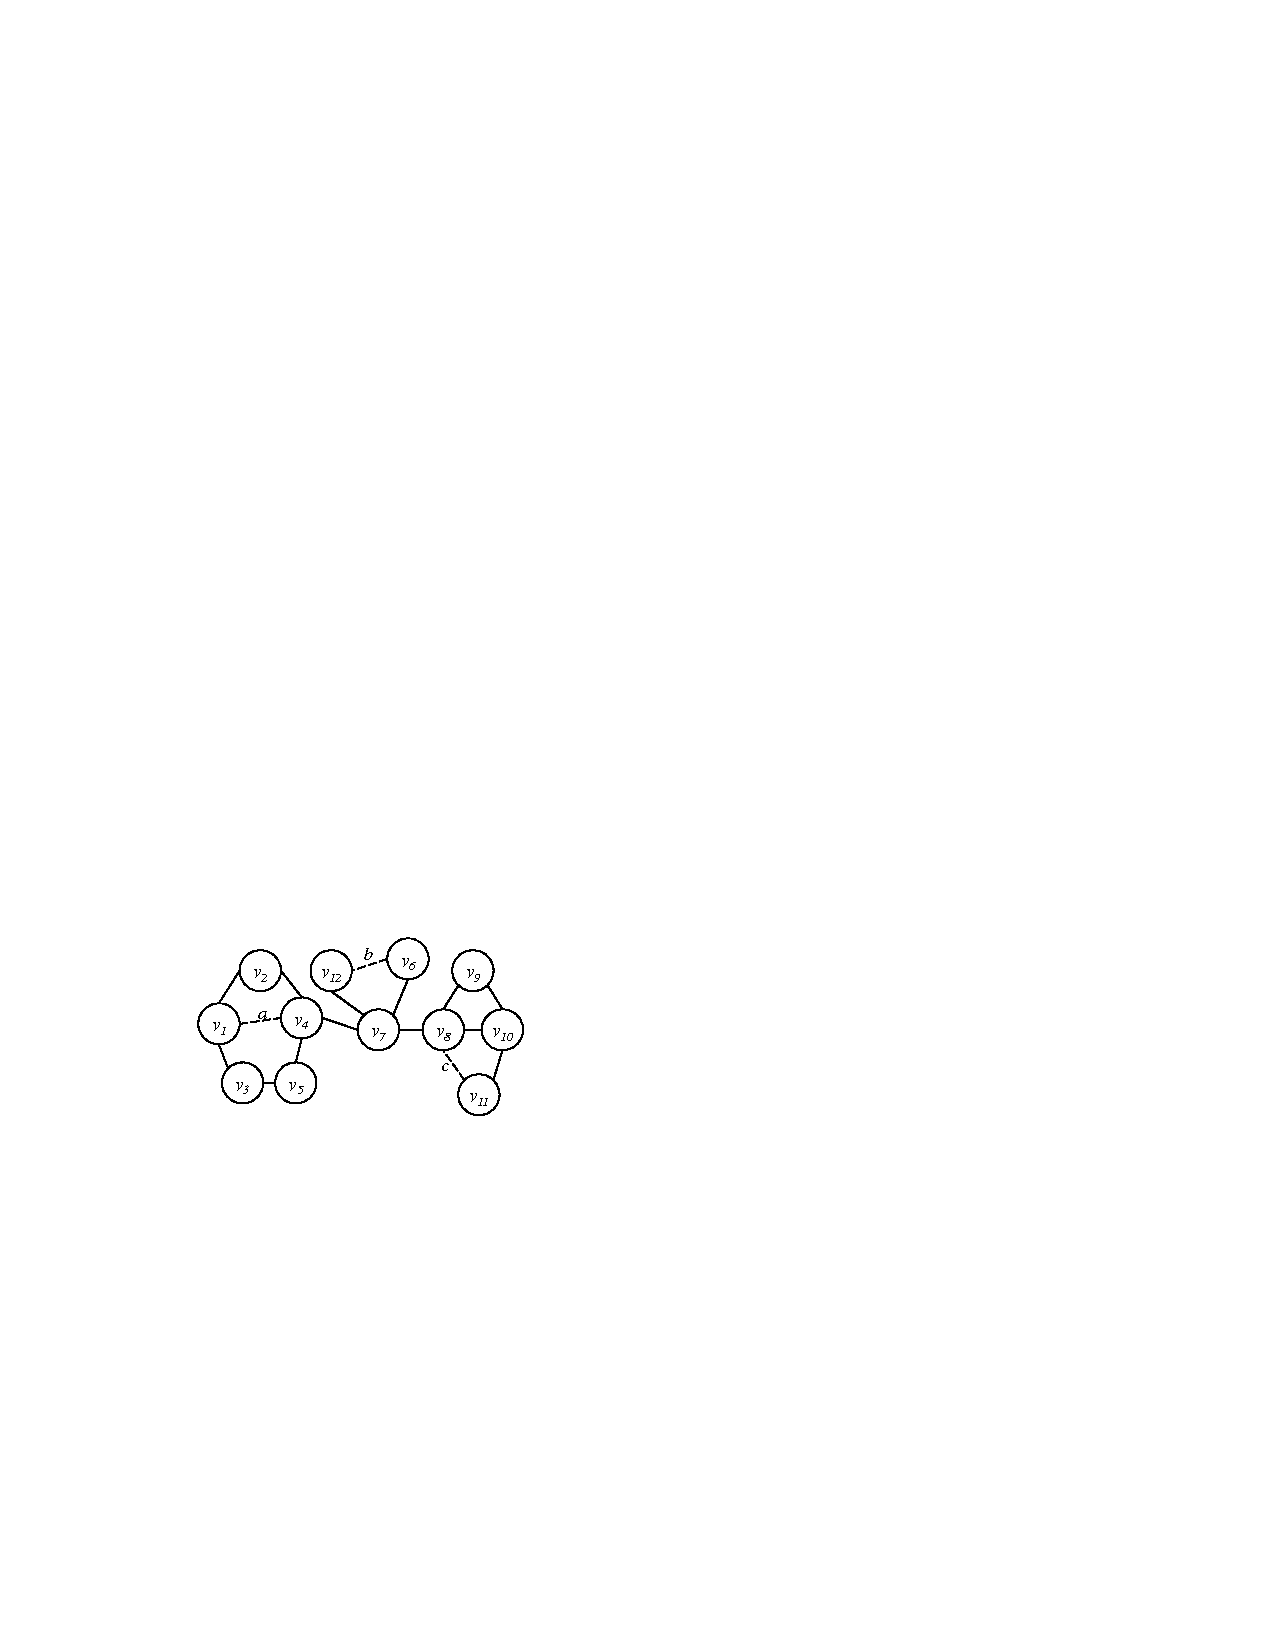
\includegraphics[width=\textwidth, height=0.5\textheight, keepaspectratio]{imgs/qube-addition}
  \end{figure}

  \begin{itemize}
    \item Adding $a$ does not affect the $MUC$ (endpoints in the same $MUC$)
    \item Adding $b$ creates a new $MUC$ (endpoints do not belong to a $MUC$)
    \item Adding $c$ merges two $MUC$s (merge $MUC$s of vertices on the \spath between endpoints)
  \end{itemize}
\end{frame}


\begin{frame}
  \frametitle{Updating MUCs -- Removal}

  \begin{figure}[t]
    \centering
    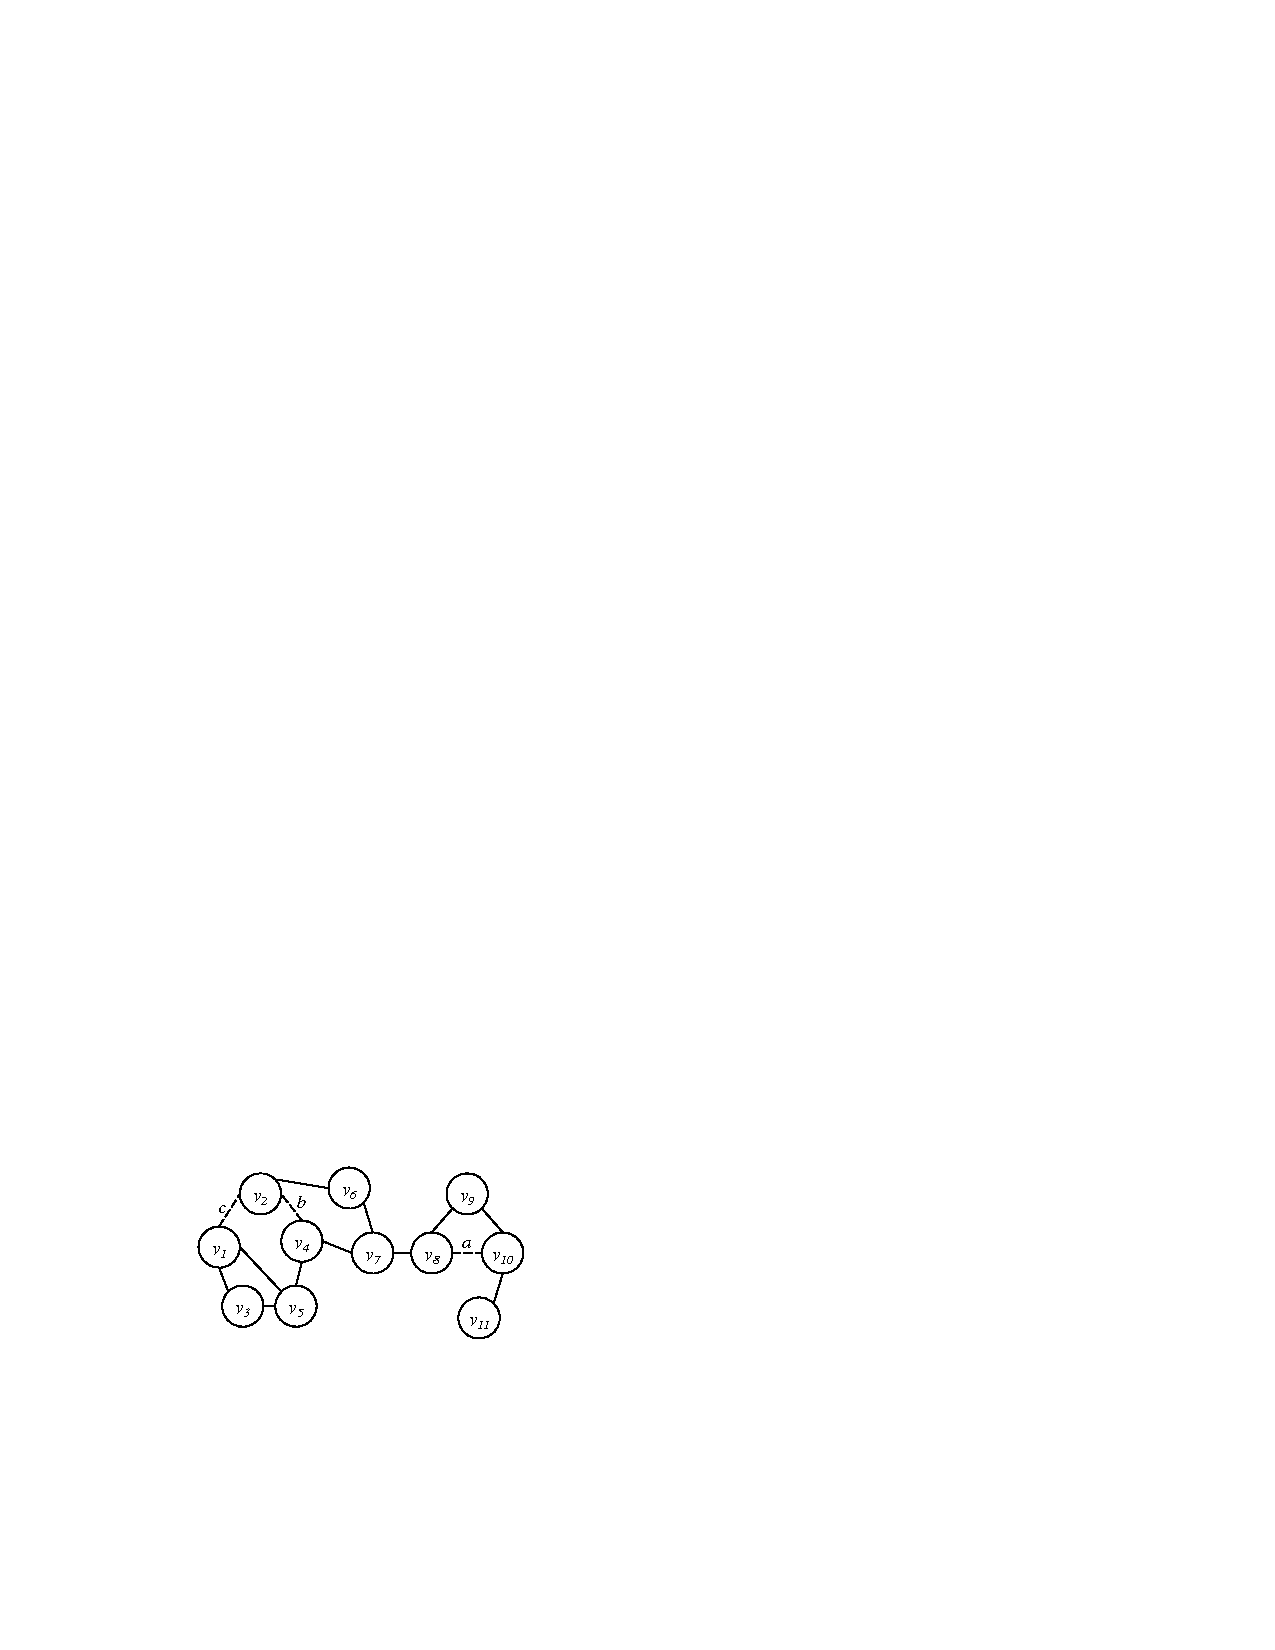
\includegraphics[width=\textwidth, height=0.5\textheight, keepaspectratio]{imgs/qube-removal}
  \end{figure}

  \begin{itemize}
    \item Removing $a$ destroys the $MUC$ (cycle is removed $\rightarrow$ no biconnected component)
    \item Removing $b$ does not affect the $MUC$ ($MUC$ is still biconnected)
    \item Removing $c$ splits the $MUC$ in two (single vertex appears in all \spath between endpoints)
  \end{itemize}
\end{frame}


\begin{frame}
  \frametitle{Betweenness Centrality Dependency}

  \begin{itemize}
    \item Only vertexes inside the $MUC$s of the updated endpoints need to be updated
    \item However, recomputing all centralities for the $MUC$ still requires new shortest paths to the rest of the graph
      \begin{itemize}
        \item Shortest paths to vertices outside the $MUC$
        \item Shortest paths that pass through the $MUC$
      \end{itemize}
  \end{itemize}

  \begin{figure}[t]
    \centering
    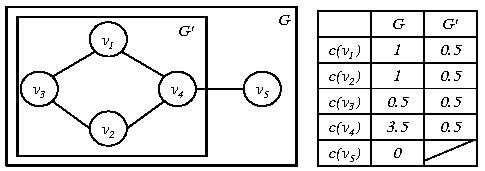
\includegraphics[width=\textwidth, height=0.6\textheight, keepaspectratio]{imgs/qube-btwmuc}
  \end{figure}
\end{frame}


\begin{frame}
  \frametitle{Betweenness Centrality outside the MUC}

  \begin{itemize}
    \item Let $s \in V_{G_j}$, $t \in MUC$,
    \item Let $j \in MUC$ be a connection vertex to subgraph $G_j$
    \item Each vertex in $\spath_{jt}$ is also in $\spath_{st}$
    \item Therefore, betweenness centrality due to vertices outside the $MUC$:
  \end{itemize}

  \begin{align*}
    %\large
    \betw_{o}(v) = \begin{cases}
      \frac{|V_{G_j}|}{\paths_{st}}		& \text{ if } v \in\{ \spath_{jt} \setminus t \} \\
      0 						& \text{ otherwise }
    \end{cases}
  \end{align*}
\end{frame}


\begin{frame}
  \frametitle{Betweenness Centrality trough the MUC}

  \begin{itemize}
    \item Let $s \in V_{G_j}$, $t \in V_{G_k}$,
    \item Let $j \in MUC$ be a connection vertex to subgraph $G_j$
    \item Let $k \in MUC$ be a connection vertex to subgraph $G_k$
    \item Each vertex in $\spath_{jk}$ is also in $\spath_{st}$
    \item Therefore, betweenness centrality due to paths through the $MUC$:
  \end{itemize}

  \begin{align*}
    \betw_{x}(v) = \begin{cases}
      \frac{ |V_{G_j}| |V_{G_k}| }{ \paths_{st} }		& \text{ if } v \in \spath_{jk} \\
      0 						& \text{ otherwise }
    \end{cases}
  \end{align*}

  More caveats apply for subgraphs that are disconnected, as every path that connects vertices in different connected component passes through $v$
\end{frame}


\begin{frame}
  \frametitle{Updating Betweenness Centrality}

  {\Large
    \begin{align*}
      \betw(v) = \betw_{MUC}(v) + \sum_{G_j \subset G} \betw_{o}(v) + \sum_{G_j, G_k \subset G} \betw_{x}(v)
    \end{align*}
  }
\end{frame}


\begin{frame}
  \frametitle{QUBE algorithm}

  \begin{figure}[t]
    \centering
    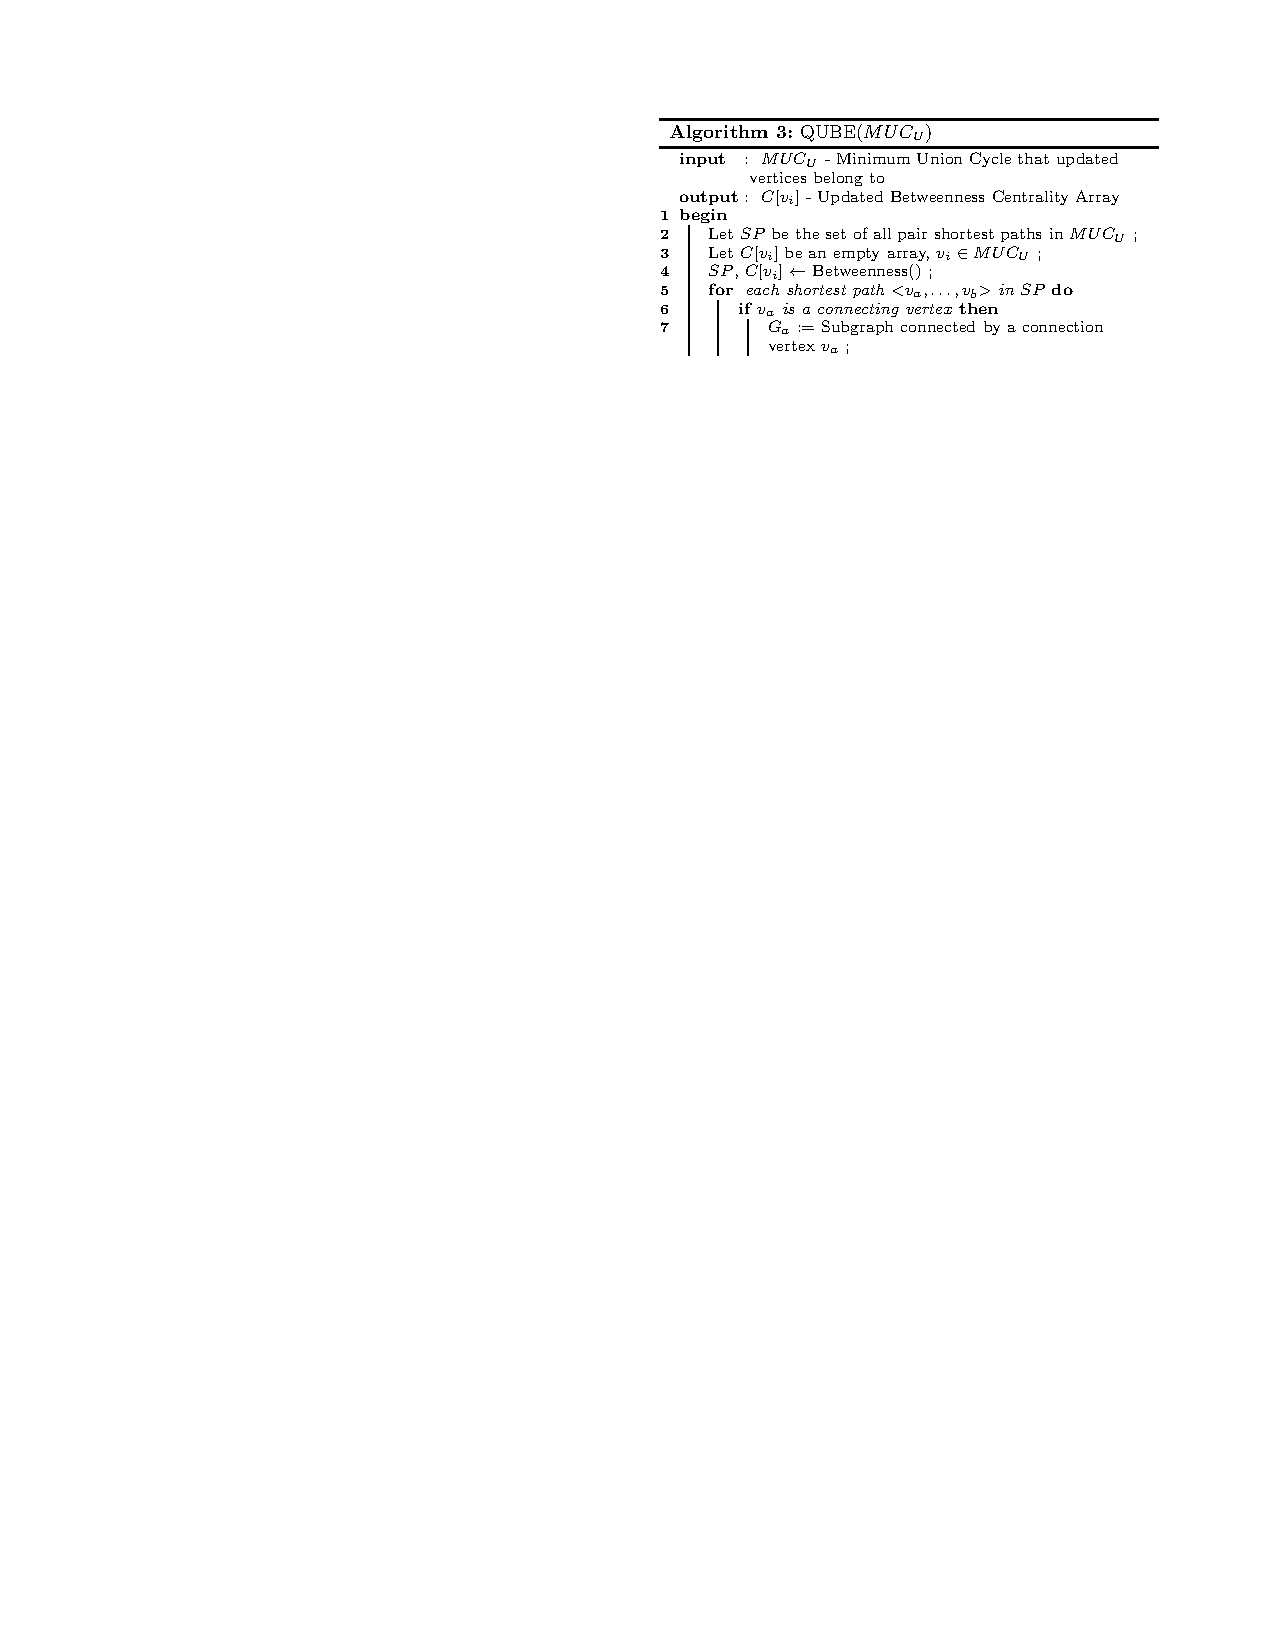
\includegraphics[width=\textwidth, height=\textheight, keepaspectratio]{imgs/qube-algorithm1}
  \end{figure}

  %  \begin{columns}[onlytextwidth]
  %    \begin{column}{0.5\textwidth}
  %      \begin{figure}[t]
  %        \centering
  %        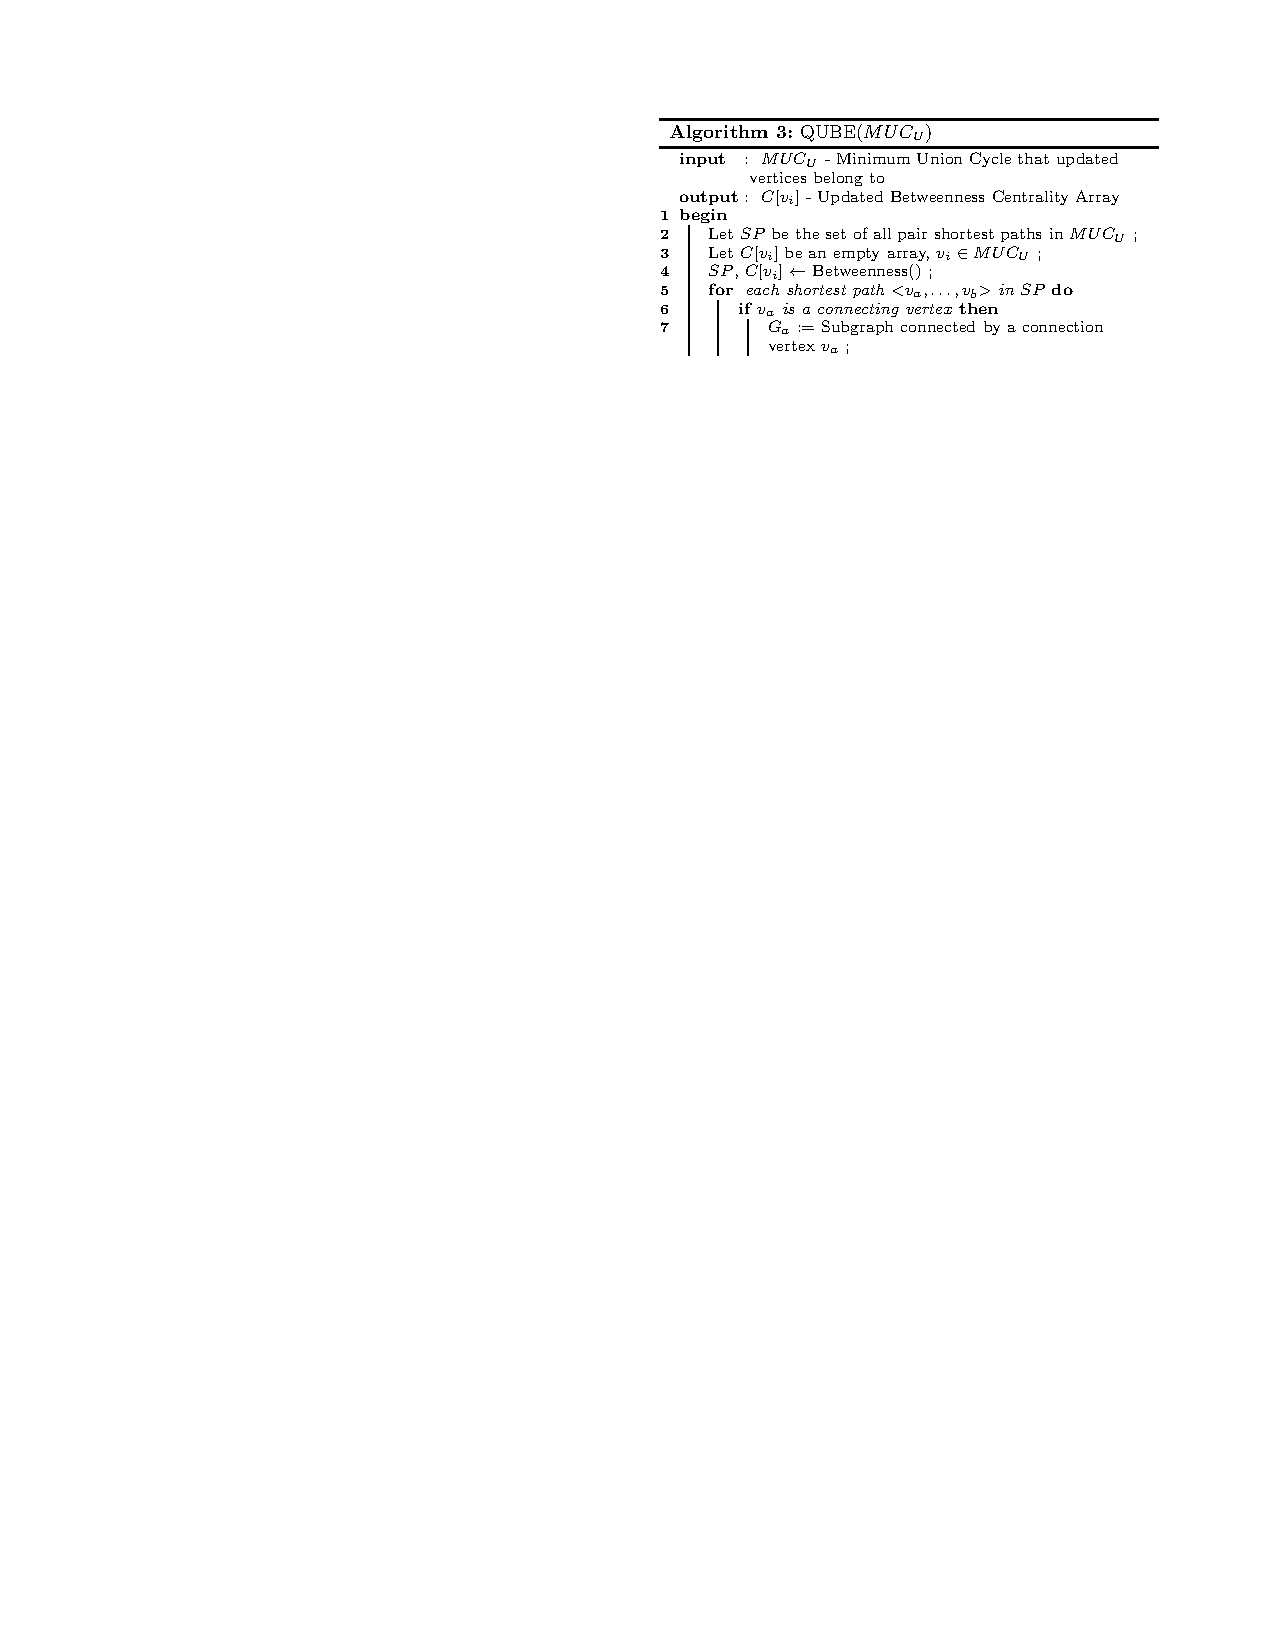
\includegraphics[width=\textwidth, height=\textheight, keepaspectratio]{imgs/qube-algorithm1}
  %      \end{figure}
  %    \end{column}

  %    \begin{column}{0.5\textwidth}
  %      \begin{figure}[t]
  %        \centering
  %        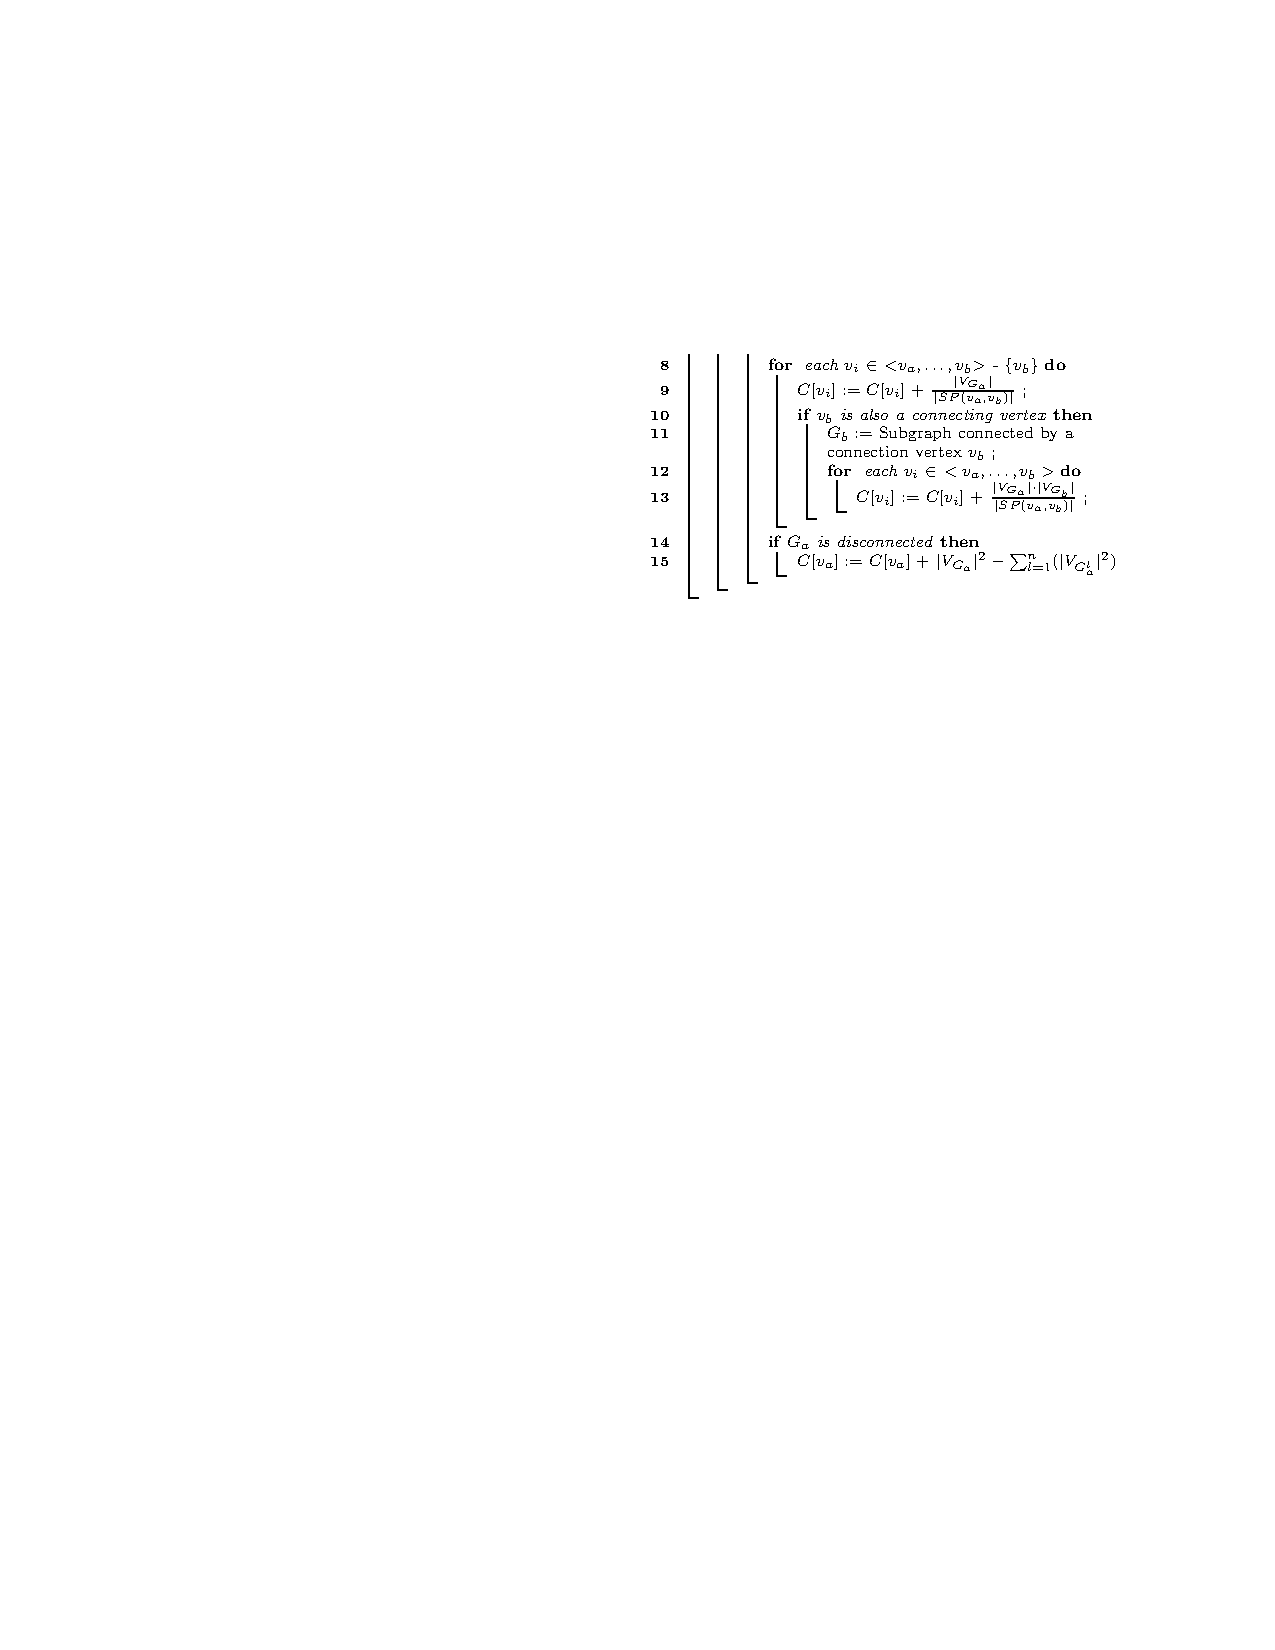
\includegraphics[width=\textwidth, height=\textheight, keepaspectratio]{imgs/qube-algorithm2}
  %      \end{figure}
  %    \end{column}
  %  \end{columns}
\end{frame}


\begin{frame}
  \frametitle{QUBE algorithm}

  \begin{figure}[t]
    \centering
    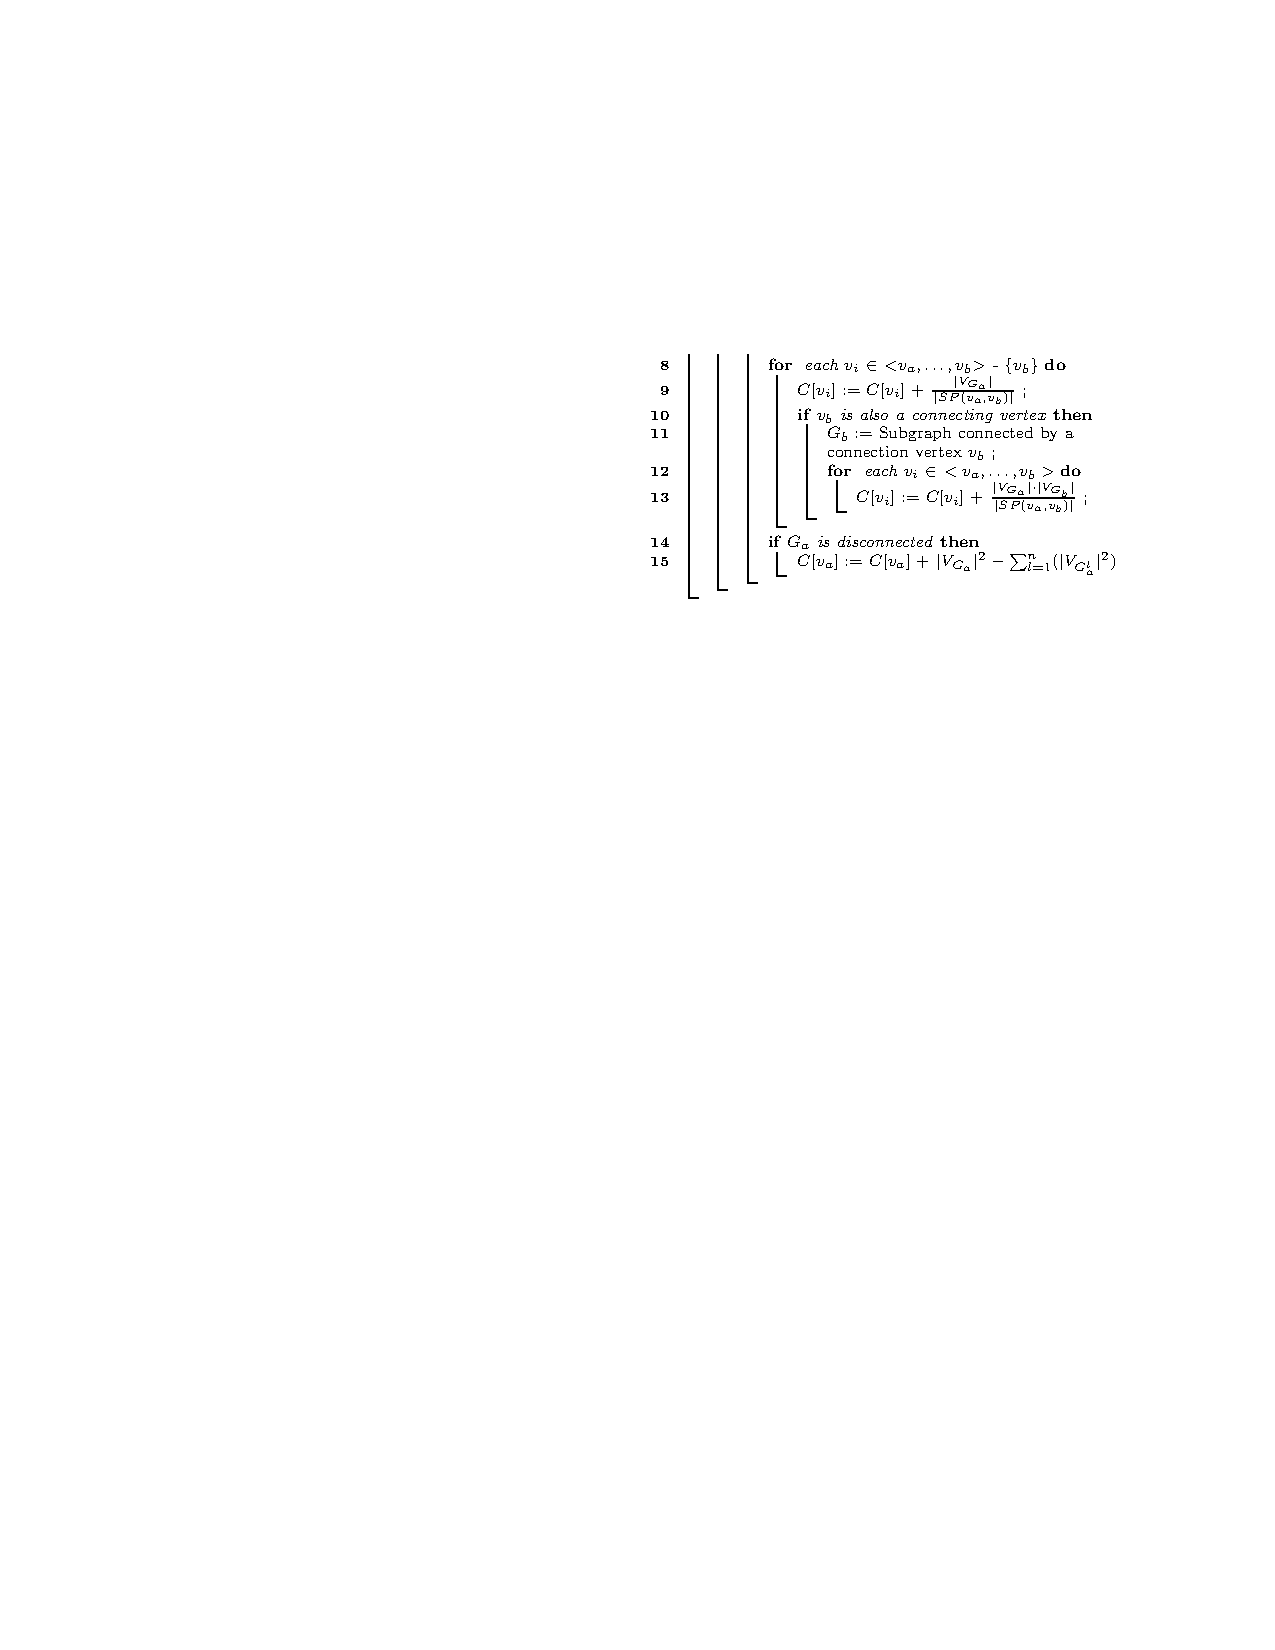
\includegraphics[width=\textwidth, height=\textheight, keepaspectratio]{imgs/qube-algorithm2}
  \end{figure}

\end{frame}


\begin{frame}
  \frametitle{QUBE + Brandes}

  \begin{itemize}
    \item QUBE is a pruning rule that reduces the search space for betweenness recomputation
    \item Can be paired with any existing betweenness algorithm to compute $\betw_{MUC}$
    \item In the experiments, Brandes' is used
    \item Quantities computed by Brandes' (e.g., \paths) reused by QUBE for $\betw_o$ and $\betw_x$
  \end{itemize}
\end{frame}


\begin{frame}
  \frametitle{Results}

  \begin{figure}[t]
    \centering
    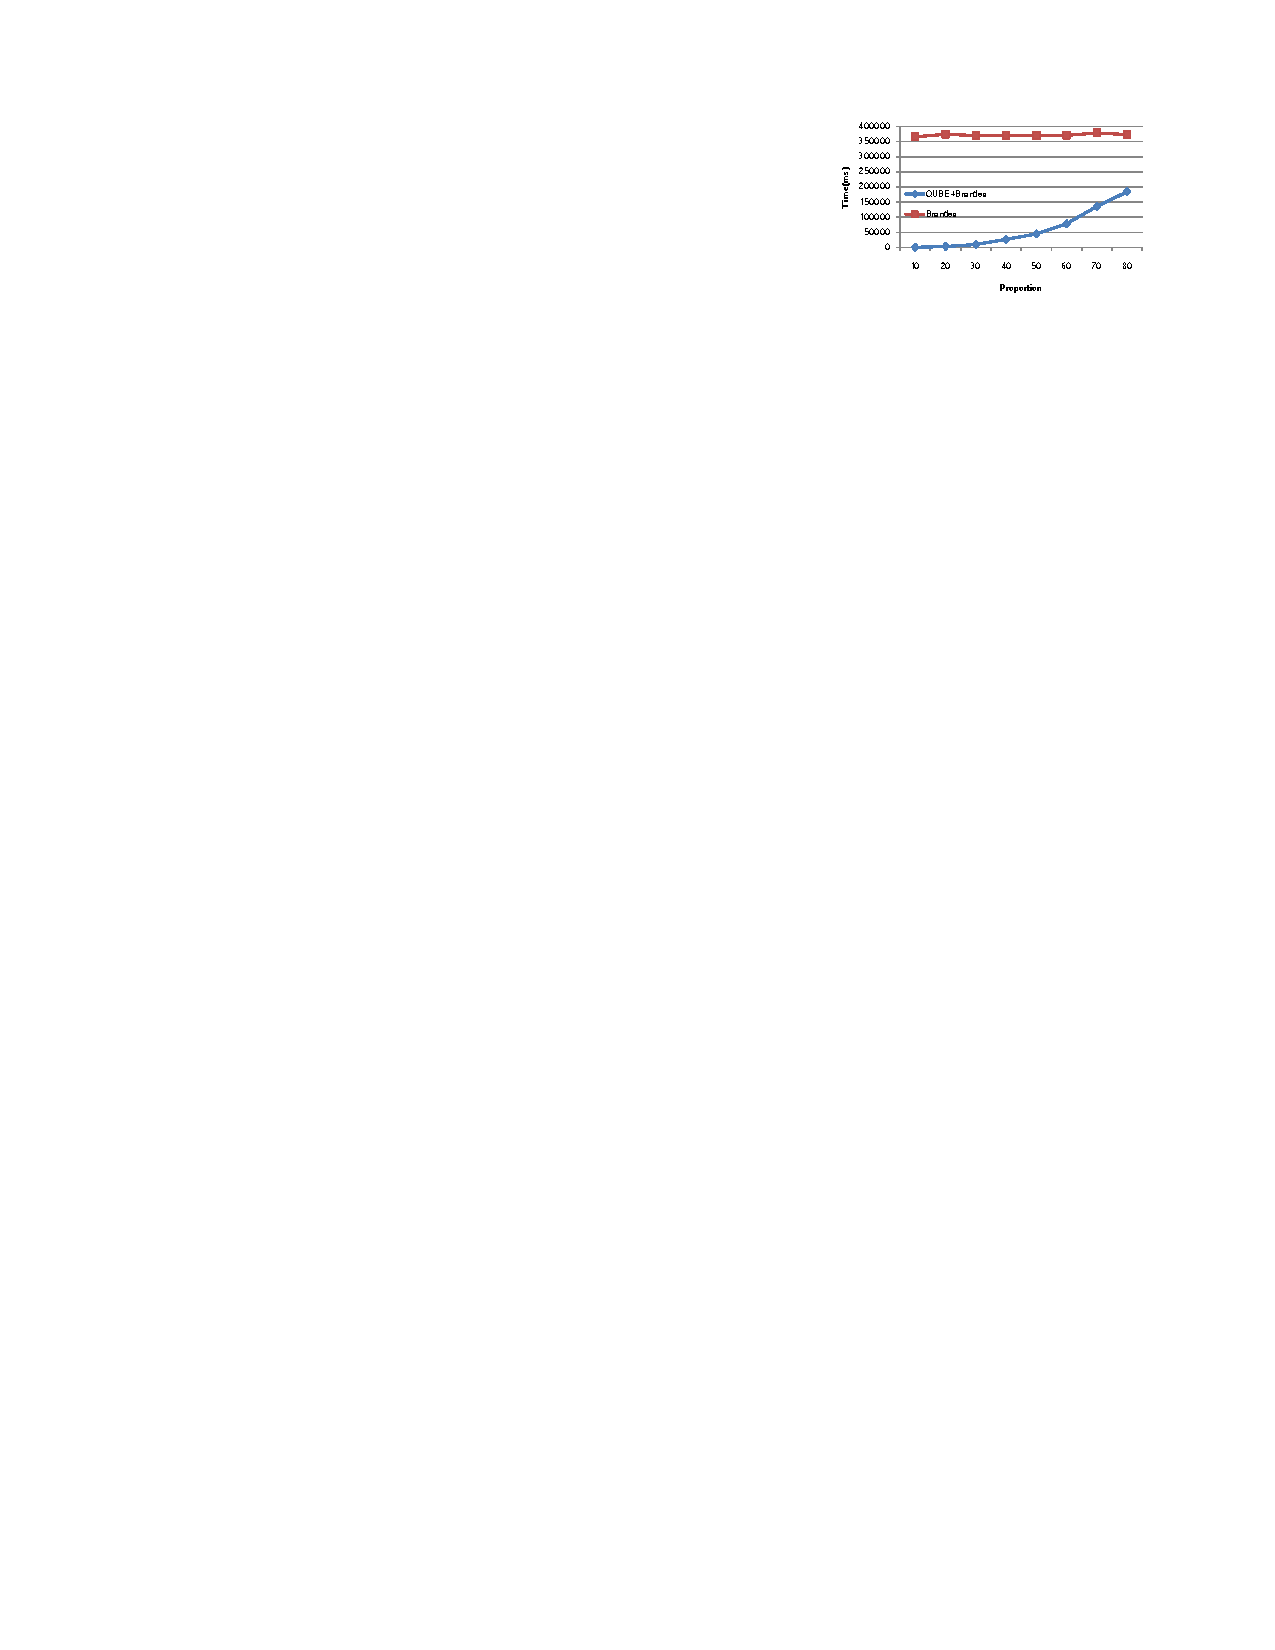
\includegraphics[width=\textwidth, height=0.7\textheight, keepaspectratio]{imgs/qube-results1}
    \caption{Update time as a function of the percentage of vertices of the graph in the updated $MUC$ for synthetic Erd\"{o}s-R\'{e}nyi graphs ($n = 5000$)}
  \end{figure}

\end{frame}


\begin{frame}
  \frametitle{Conclusions}

  \begin{figure}[t]
    \centering
    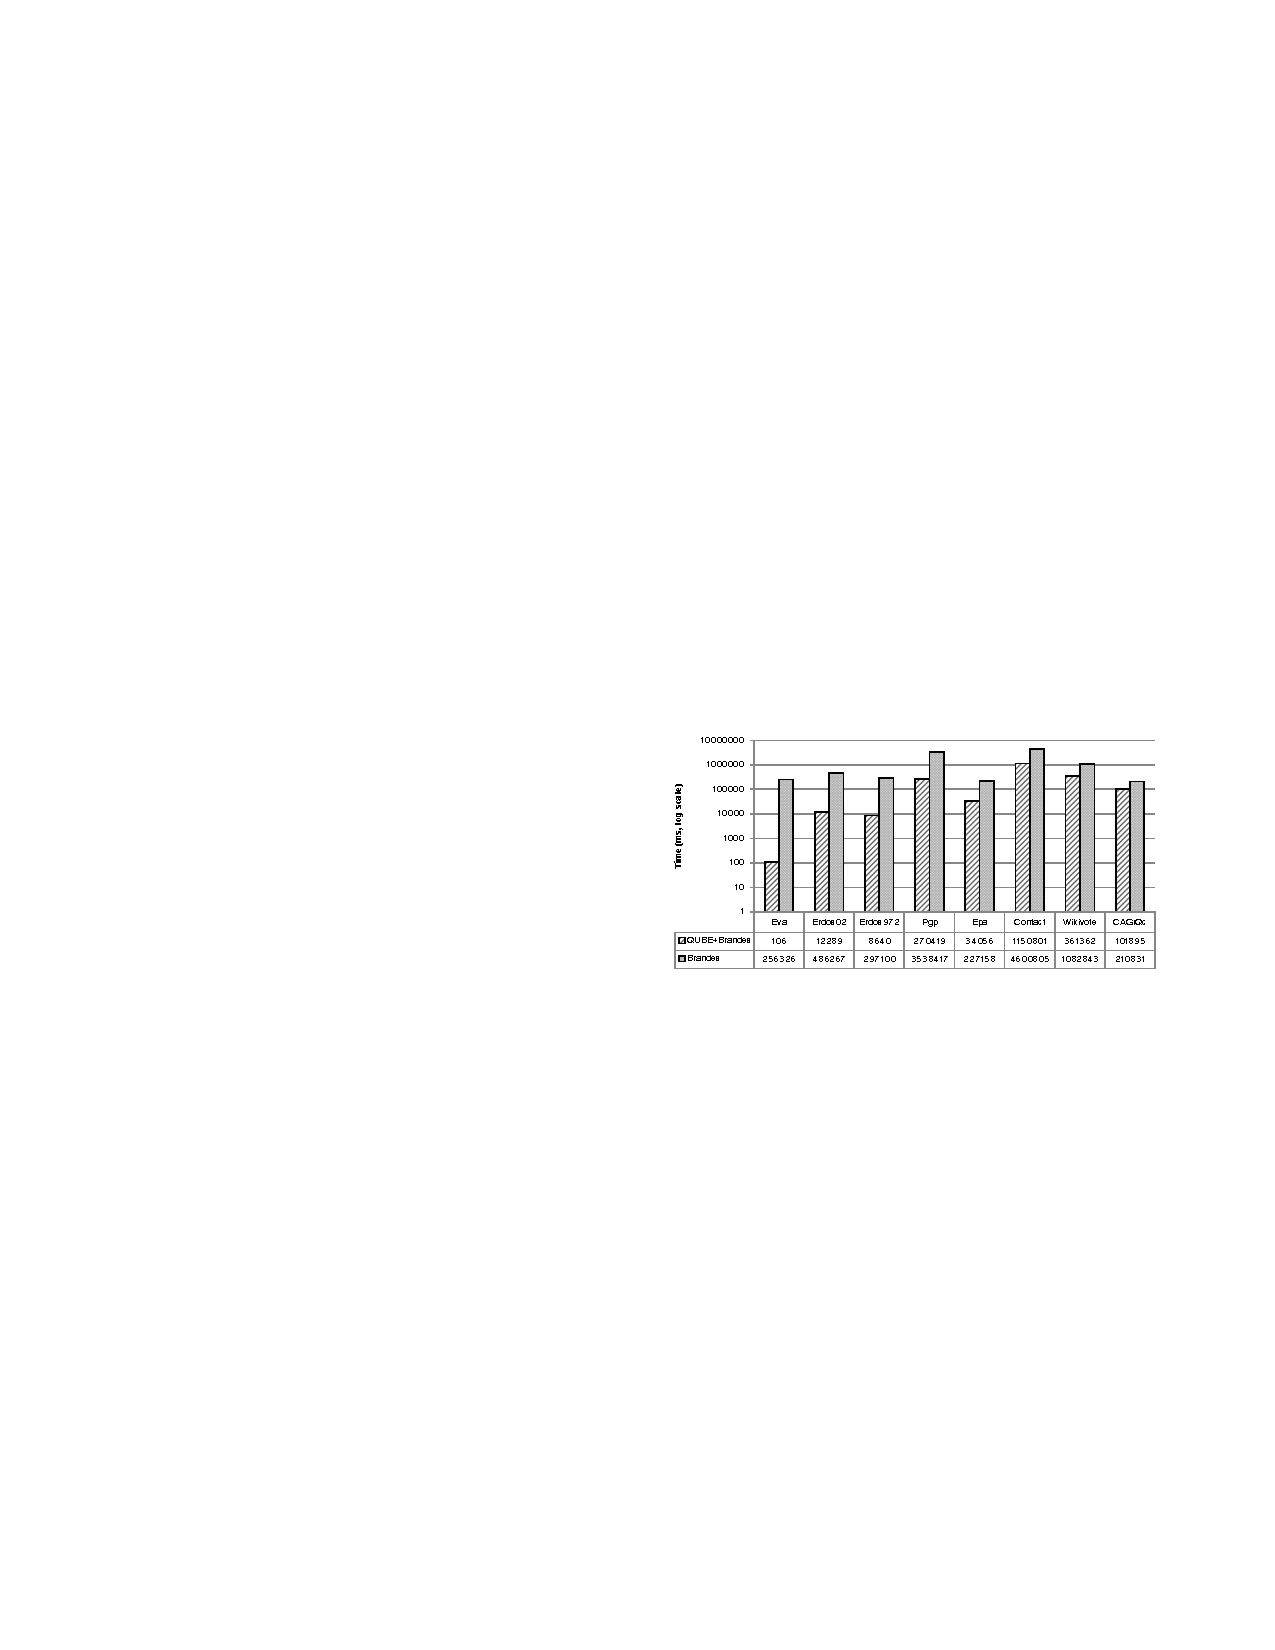
\includegraphics[width=\textwidth, height=0.6\textheight, keepaspectratio]{imgs/qube-results2}
  \end{figure}

  \begin{itemize}
    \item Improvement depends highly on structure of the graph (bi-connectedness)
    \item From 2 orders of magnitude (best) to 2 times (worst) faster than Brandes'
  \end{itemize}

\end{frame}


%% Kas et al.
\begin{frame}
  \centering
  \vfill
  {\huge Incremental Algorithm for Updating Betweenness Centrality in Dynamically Growing Networks}
  \vfill
  {\Large M. Kas, M. Wachs, K. M. Carley, L. R. Carley}
  \vfill
  {\large ASONAM '13: International Conference on Advances \\in Social Networks analysis and Mining}
  \vfill
\end{frame}


\begin{frame}
  \frametitle{Intuition}

  \begin{itemize}
    \item Extend an existing dynamic all-pairs shortest path algorithm to betweenness
    \item G. Ramalingam and T. Reps, ``\emph{On the Computational Complexity of Incremental Algorithms},'' CS, Univ. of Wisconsin at Madison, Tech. Report 1991
    \item Relevant quantities: number of shortest paths \paths, distances \dist, predecessors \pred
    \item Keep a copy of the old quantities while updating
    \item Support only edge addition (on weighted graphs)
  \end{itemize}

\end{frame}


\begin{frame}
  \frametitle{Edge update}

  \begin{itemize}
    \item Compute new shortest paths from updated endpoints $(u,v)$
    \item If a new shortest path of the same length is found, updated number of paths as
  \end{itemize}
  {\Large
    \begin{align*}
      \paths_{st} = \paths_{st} + \paths_{su} \times \paths_{vt}
    \end{align*}
  }
  \begin{itemize}
    \item If a new \emph{shorter} shortest path to any vertex is found, update \dist, clear \paths
    \item Betweenness decreased if new shortest path found
    \item Edge betweenness updates backtrack via DFS over $\pred_s(t)$
  \end{itemize}
  {\Large
    \begin{align*}
      \betw(w) = \betw(w) - \paths_{sw} \times \paths_{wt} / \paths_{st}
    \end{align*}
  }
\end{frame}


\begin{frame}
  \frametitle{Edge update}

  \begin{itemize}
    \item Complex bookkeeping: need to consider all affected vertices which have new alternative shortest paths of equal length (not covered in the original algorithm)
    \item Amend \pred during update propagation $\rightarrow$ concurrent changes to the \spdag
    \item Need to track now-unreachable vertices separately
  \end{itemize}

  \begin{itemize}
    \item After having fixed \dist, \paths, \betw, increase \betw due to new paths
    \item Update needed $\forall s,t \in V$ affected by changes (tracked from previous phase)
    \item Betweenness increase analogous to above decrease
  \end{itemize}
\end{frame}


\begin{frame}
  \frametitle{Results}

  \begin{figure}[t]
    \centering
    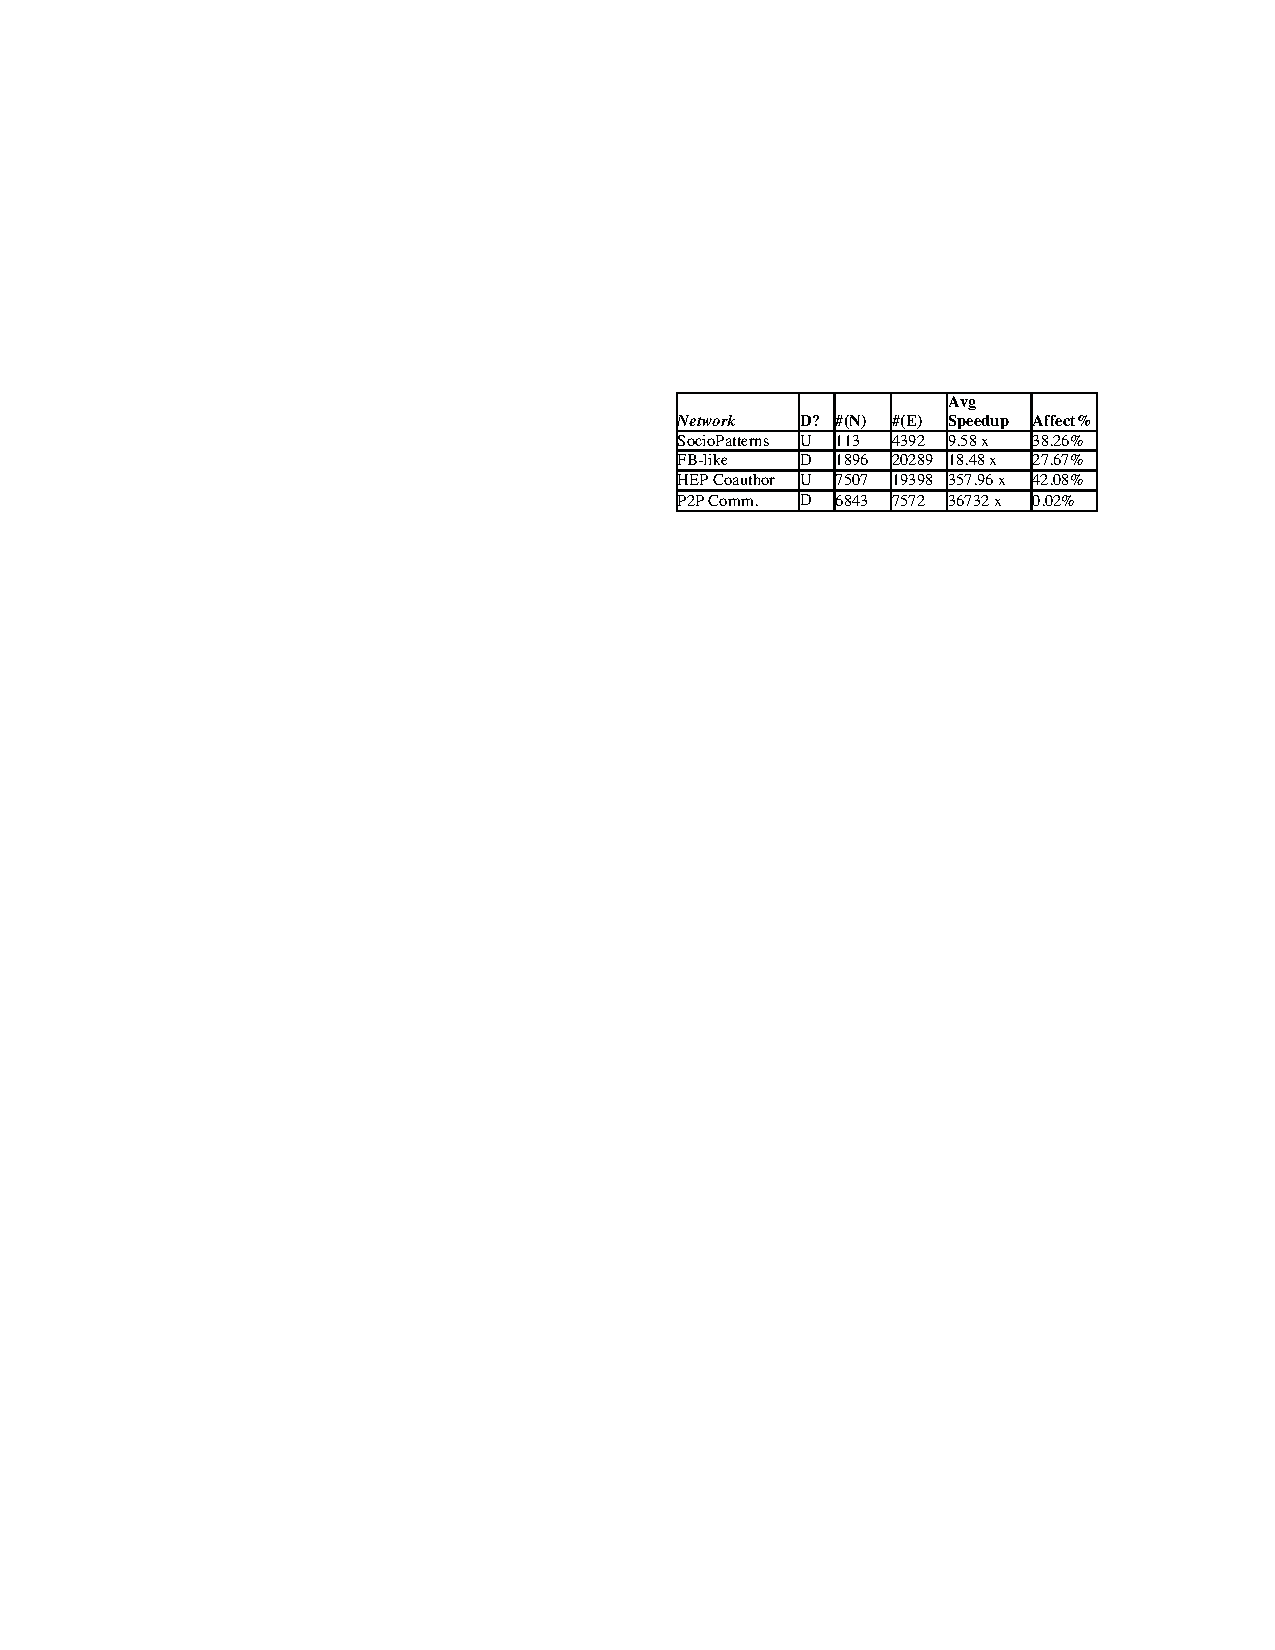
\includegraphics[width=\textwidth, height=0.7\textheight, keepaspectratio]{imgs/kas-results1}
    \caption{Speedup over Brandes' on real-world graphs}
  \end{figure}

  \begin{itemize}
    \item Speedup depends on topological characteristics (e.g., diameter, clust. coeff.)
  \end{itemize}

\end{frame}


\begin{frame}
  \frametitle{Comparison with QUBE}

  \begin{figure}[t]
    \centering
    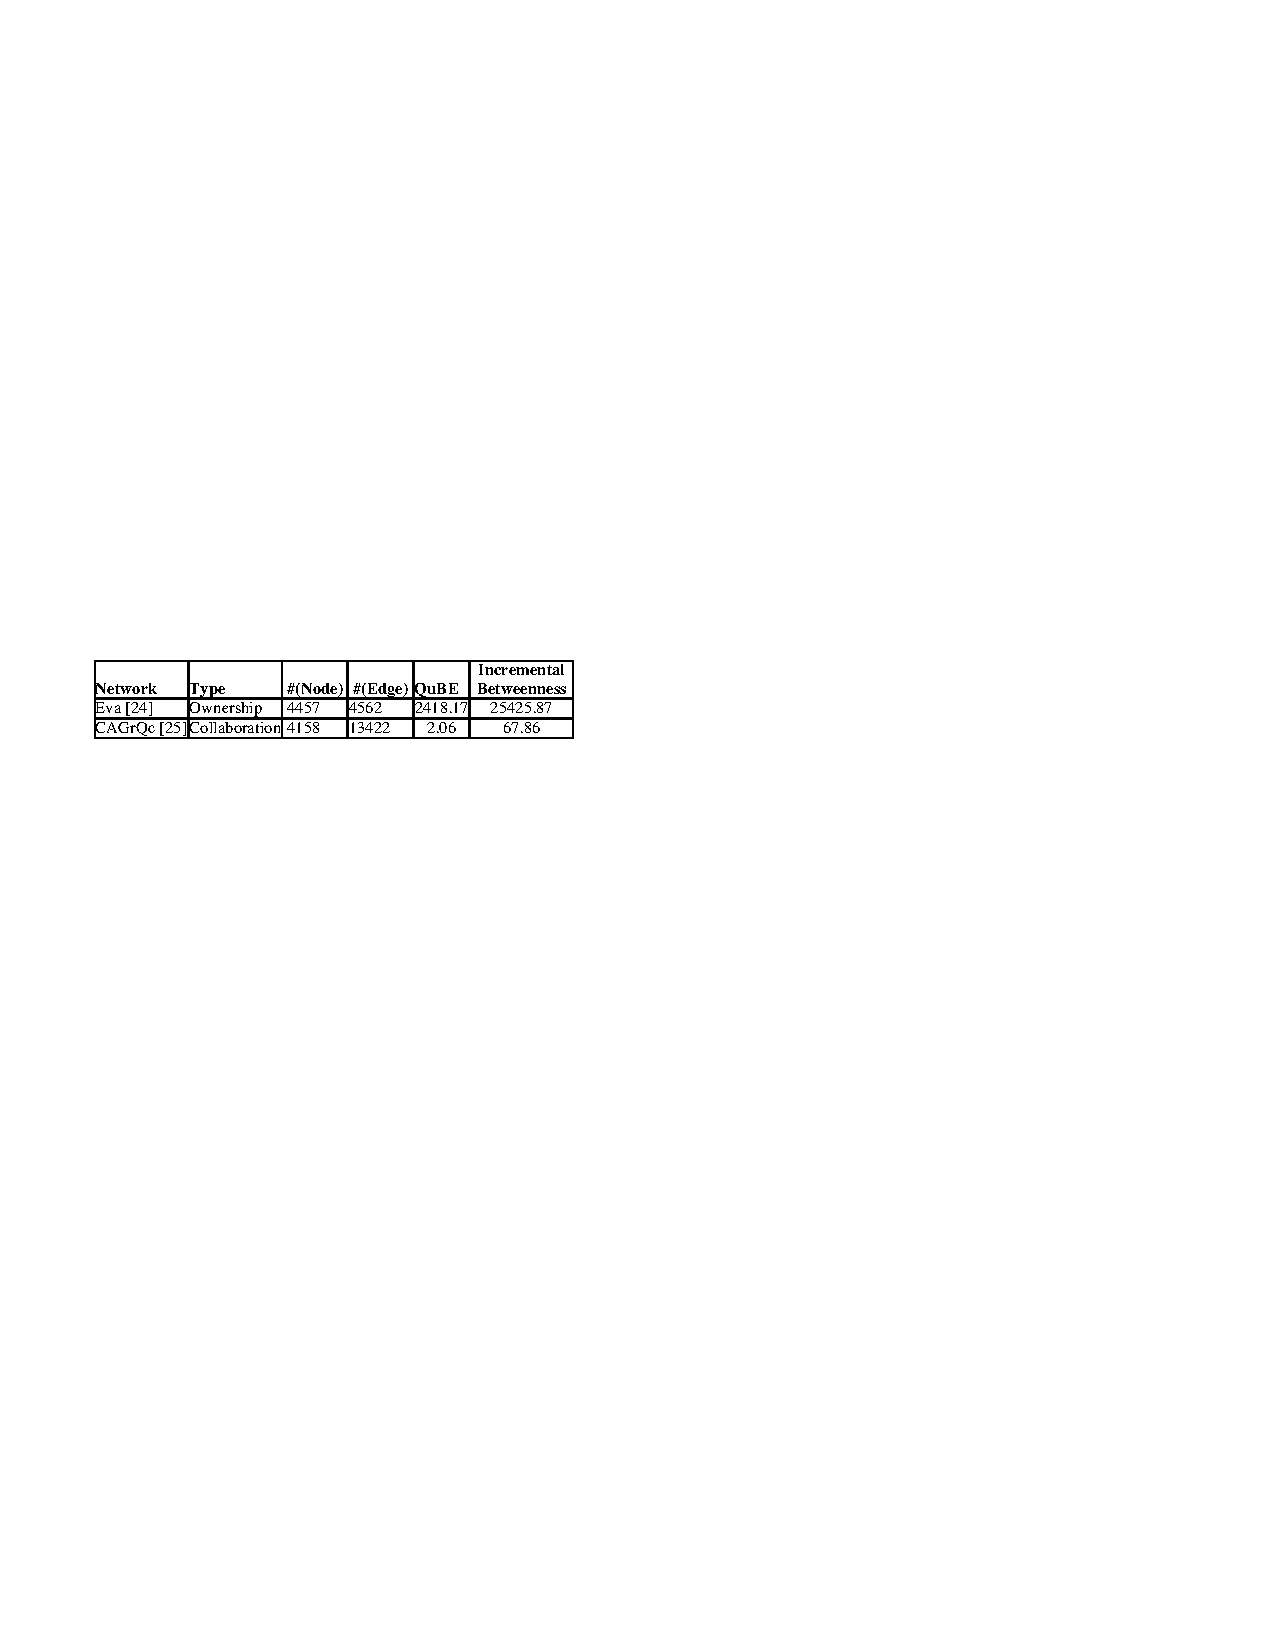
\includegraphics[width=\textwidth, height=0.7\textheight, keepaspectratio]{imgs/kas-results2}
    \caption{Speedup over Brandes' in comparison with QUBE}
  \end{figure}

  \begin{itemize}
    \item Datasets from the QUBE paper
    \item About 1 order of magnitude faster than QUBE
  \end{itemize}

\end{frame}


%% Nasre et al.
\begin{frame}
  \centering
  \vfill
  {\huge Betweenness Centrality -- Incremental and Faster}
  \vfill
  {\Large M. Nasre, M. Pontecorvi, V. Ramachandran}
  \vfill
  {\large MFCS '14: Mathematical Foundations of Computer Science}
  \vfill
\end{frame}


\begin{frame}
  \frametitle{Intuition}

  \begin{itemize}
    \item Keep \spdag for each vertex
    \item Re-use information from \spdag of updated edge endpoints
    \item Adding new edges will \emph{not} make old edges part of a \spath
    \item Support only edge addition (on weighted graphs)
  \end{itemize}

\end{frame}


\begin{frame}
  \frametitle{Main Result}

  %  \begin{figure}[H]
  %    \centering
  %    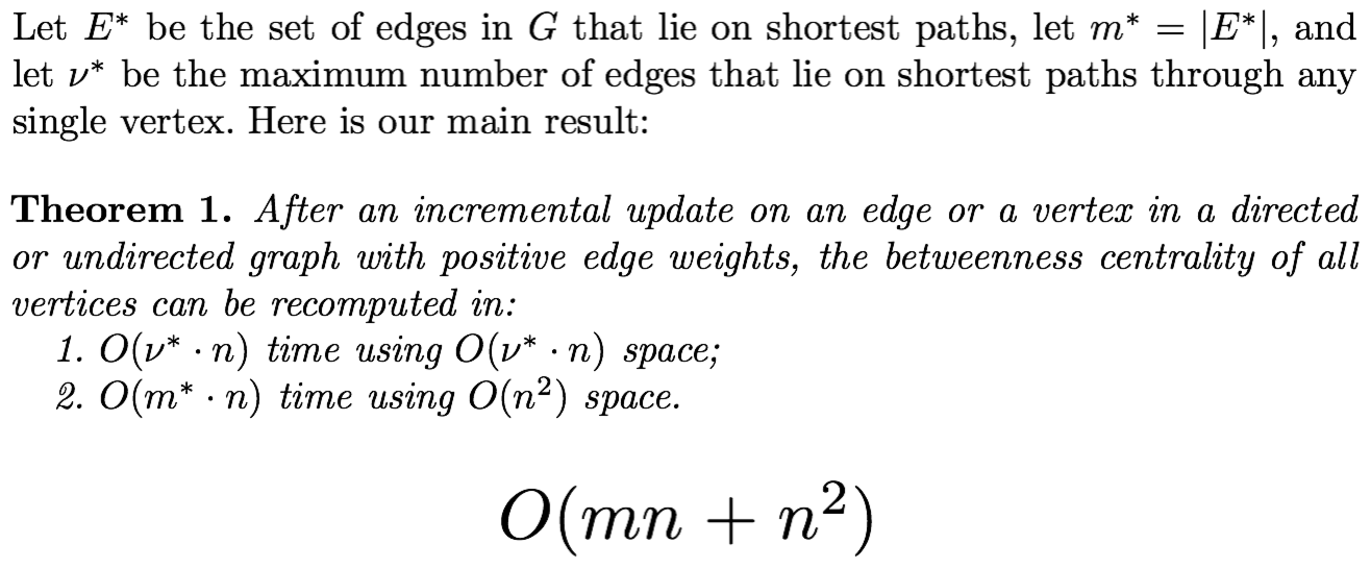
\includegraphics[width=0.5\textwidth]{imgs/npr14-main-result}
  %  \end{figure}

  \begin{itemize}
    \item Let $\displaystyle E^* = \bigcup_{e \in \allspath} e \subseteq E$ be the set of edges that are part of any shortest path
    \item Let $\displaystyle m^* = |E^*|$ and $\displaystyle \nu^* = \max_{v \in V} |\spdag_v|$ the maximum number of edges in shortest paths through any single vertex $v$
    \item $n < \nu^* < m^* < m$
    \item After incremental update, betweenness can be recomputed in
      \begin{itemize}
        \item $O(\nu^* n)$ time using $O(\nu^* n)$ space
        \item $O(m^* n)$ time using $O(n^2)$ space
      \end{itemize}
    \item Bounded by $O(mn + n^2)$
    \item Logarithmic factor better than Brandes' (on weighted graphs)
  \end{itemize}
\end{frame}


\begin{frame}
  \frametitle{Lemma 1}

  \begin{figure}[H]
    \centering
    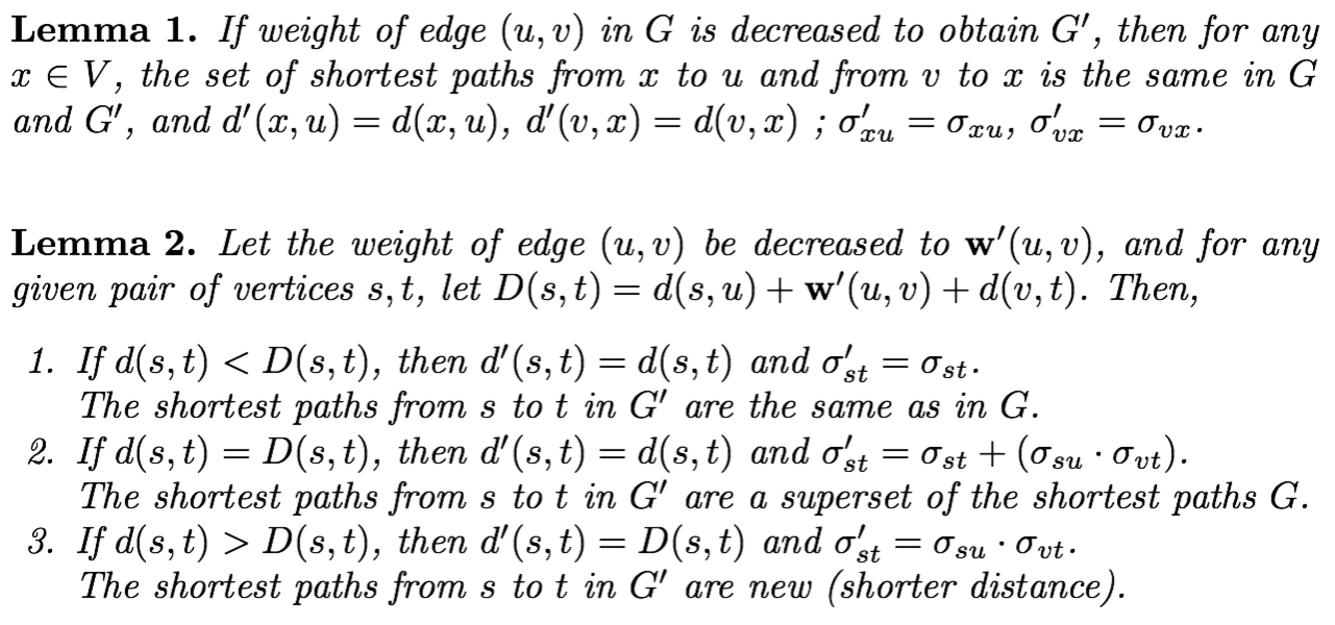
\includegraphics[width=\textwidth, trim={0 8cm 0 0}, clip]{imgs/npr14-lemmas}
  \end{figure}

  \begin{itemize}
    \item Edge $(u,v) \not\in \spath_{xu} \, \wedge \, (u,v)\not\in \spath_{vx}$ as edge weights are positive
  \end{itemize}
\end{frame}


\begin{frame}
  \frametitle{Lemma 2}

  \begin{figure}[H]
    \centering
    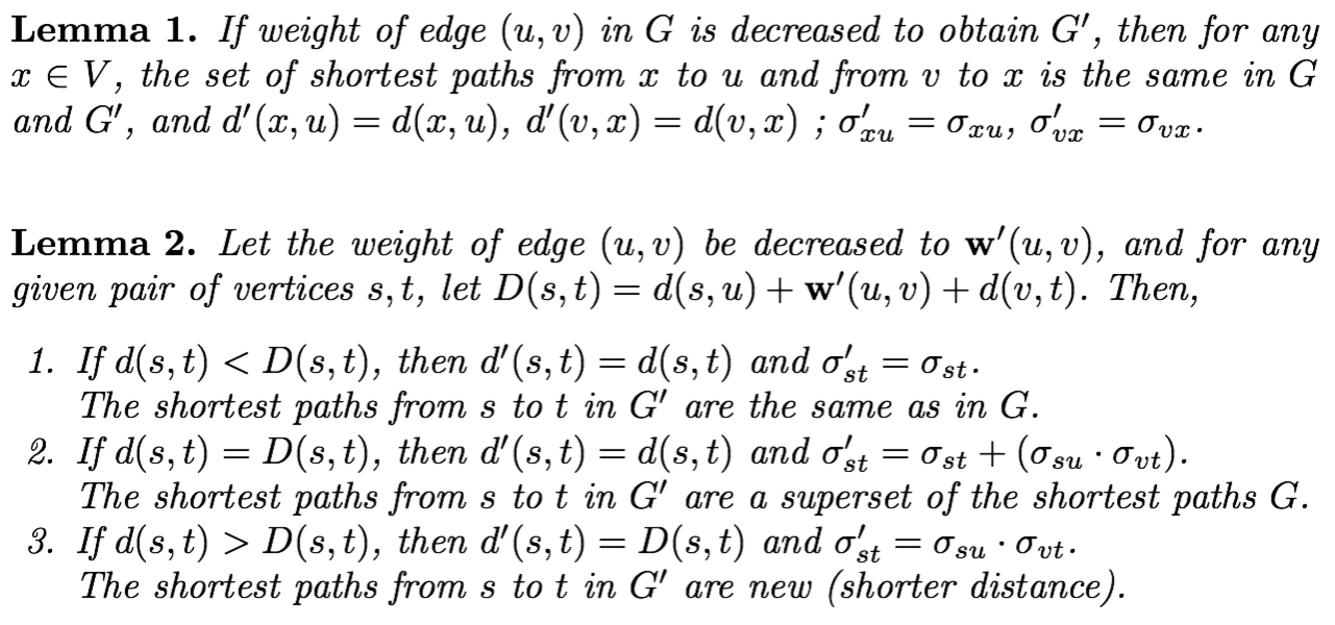
\includegraphics[width=\textwidth, trim={0 0 0 3.5cm}, clip]{imgs/npr14-lemmas}
  \end{figure}

  \begin{itemize}
    \item Updates to \paths and \dist in constant time
    \item Need to update \pred to complete \spdag update
  \end{itemize}
\end{frame}


\begin{frame}
  \frametitle{\spdag Update}

  \begin{figure}[H]
    \centering
    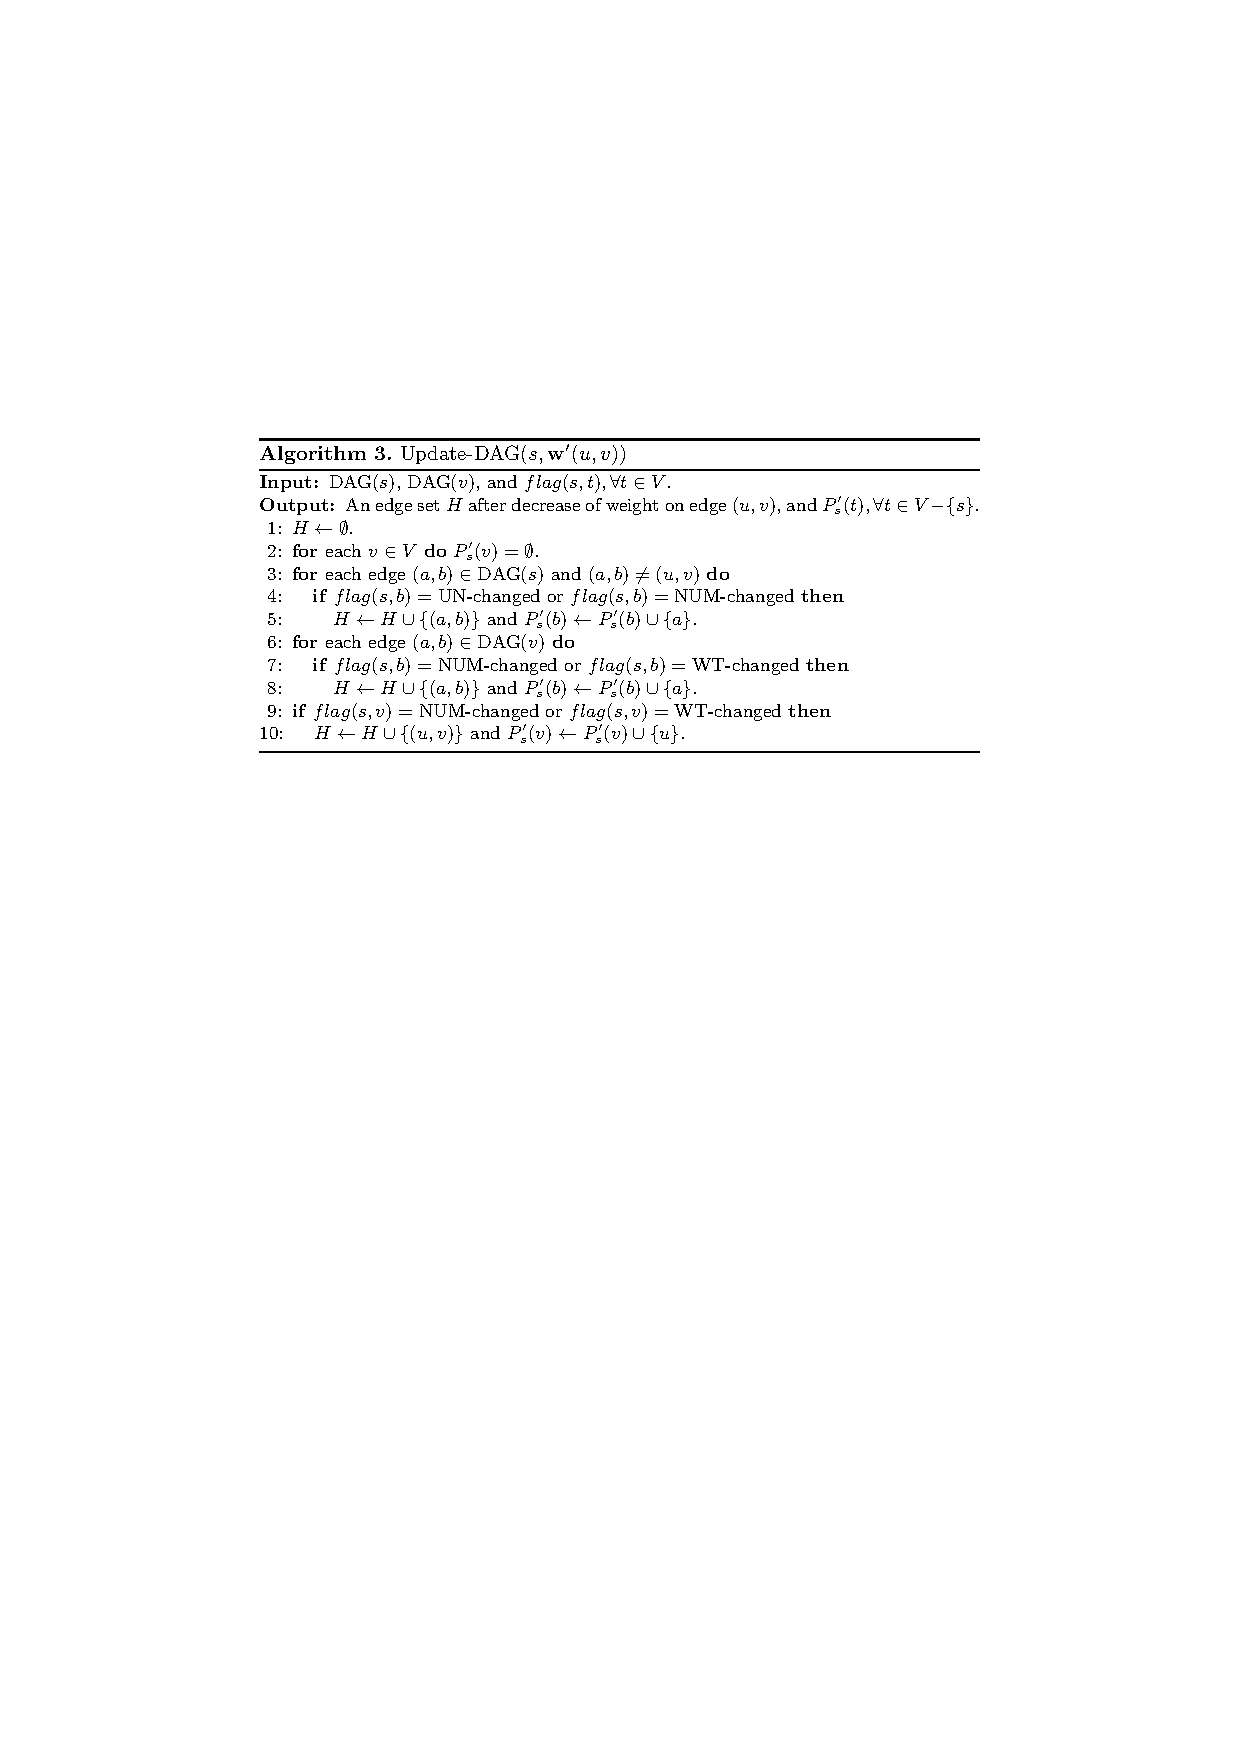
\includegraphics[width=\textwidth]{imgs/npr14-algo3}
  \end{figure}

  \begin{itemize}
    \item UN-changed $\rightarrow dd=0$
    \item NUM-changed $\rightarrow dd=1$
    \item WT-changed $\rightarrow dd>1$
  \end{itemize}
\end{frame}


\begin{frame}
  \frametitle{Edge Update}

  \begin{figure}[H]
    \centering
    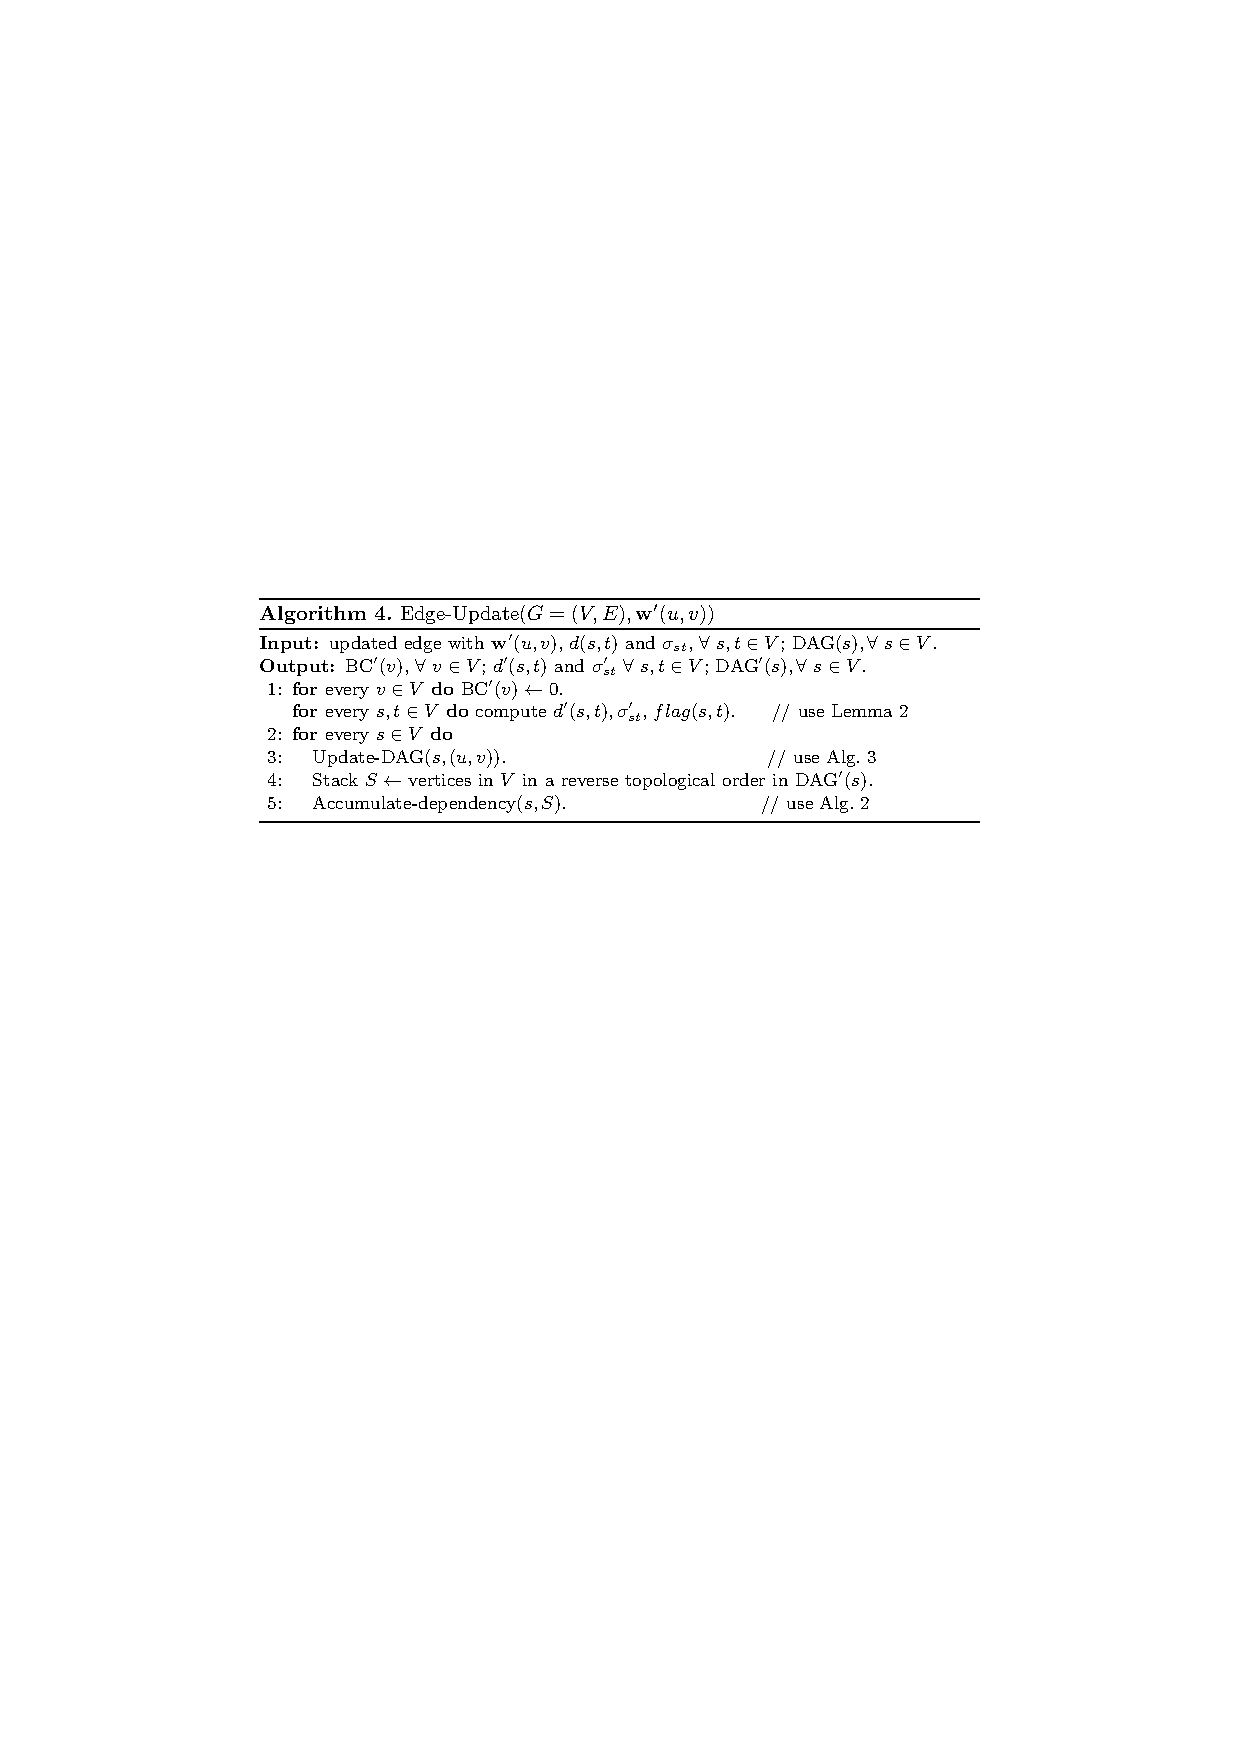
\includegraphics[width=\textwidth]{imgs/npr14-algo4}
  \end{figure}
\end{frame}


\begin{frame}
  \frametitle{Space-Efficient Variant $O(n^2)$}

  \begin{itemize}
    \item Do not store the \spdag
    \item Store only $E^*$
    \item Updated \spdag can be build in $O(m^*)$ time
      \begin{itemize}
        \item Time $O(m^* \, n)$
        \item Compute ${E'}^*$ from $E^*$, then $\spdag'_{s}$ from ${E'}^*$
      \end{itemize}
    \item Space $O(m^* + n^2)$ to store $E^*$ and $n^2$ distances $\dist(s,t)$ and shortest paths $\paths_{st}$
  \end{itemize}
\end{frame}


\begin{frame}
  \frametitle{Comparison}

  \begin{figure}[H]
    \centering
    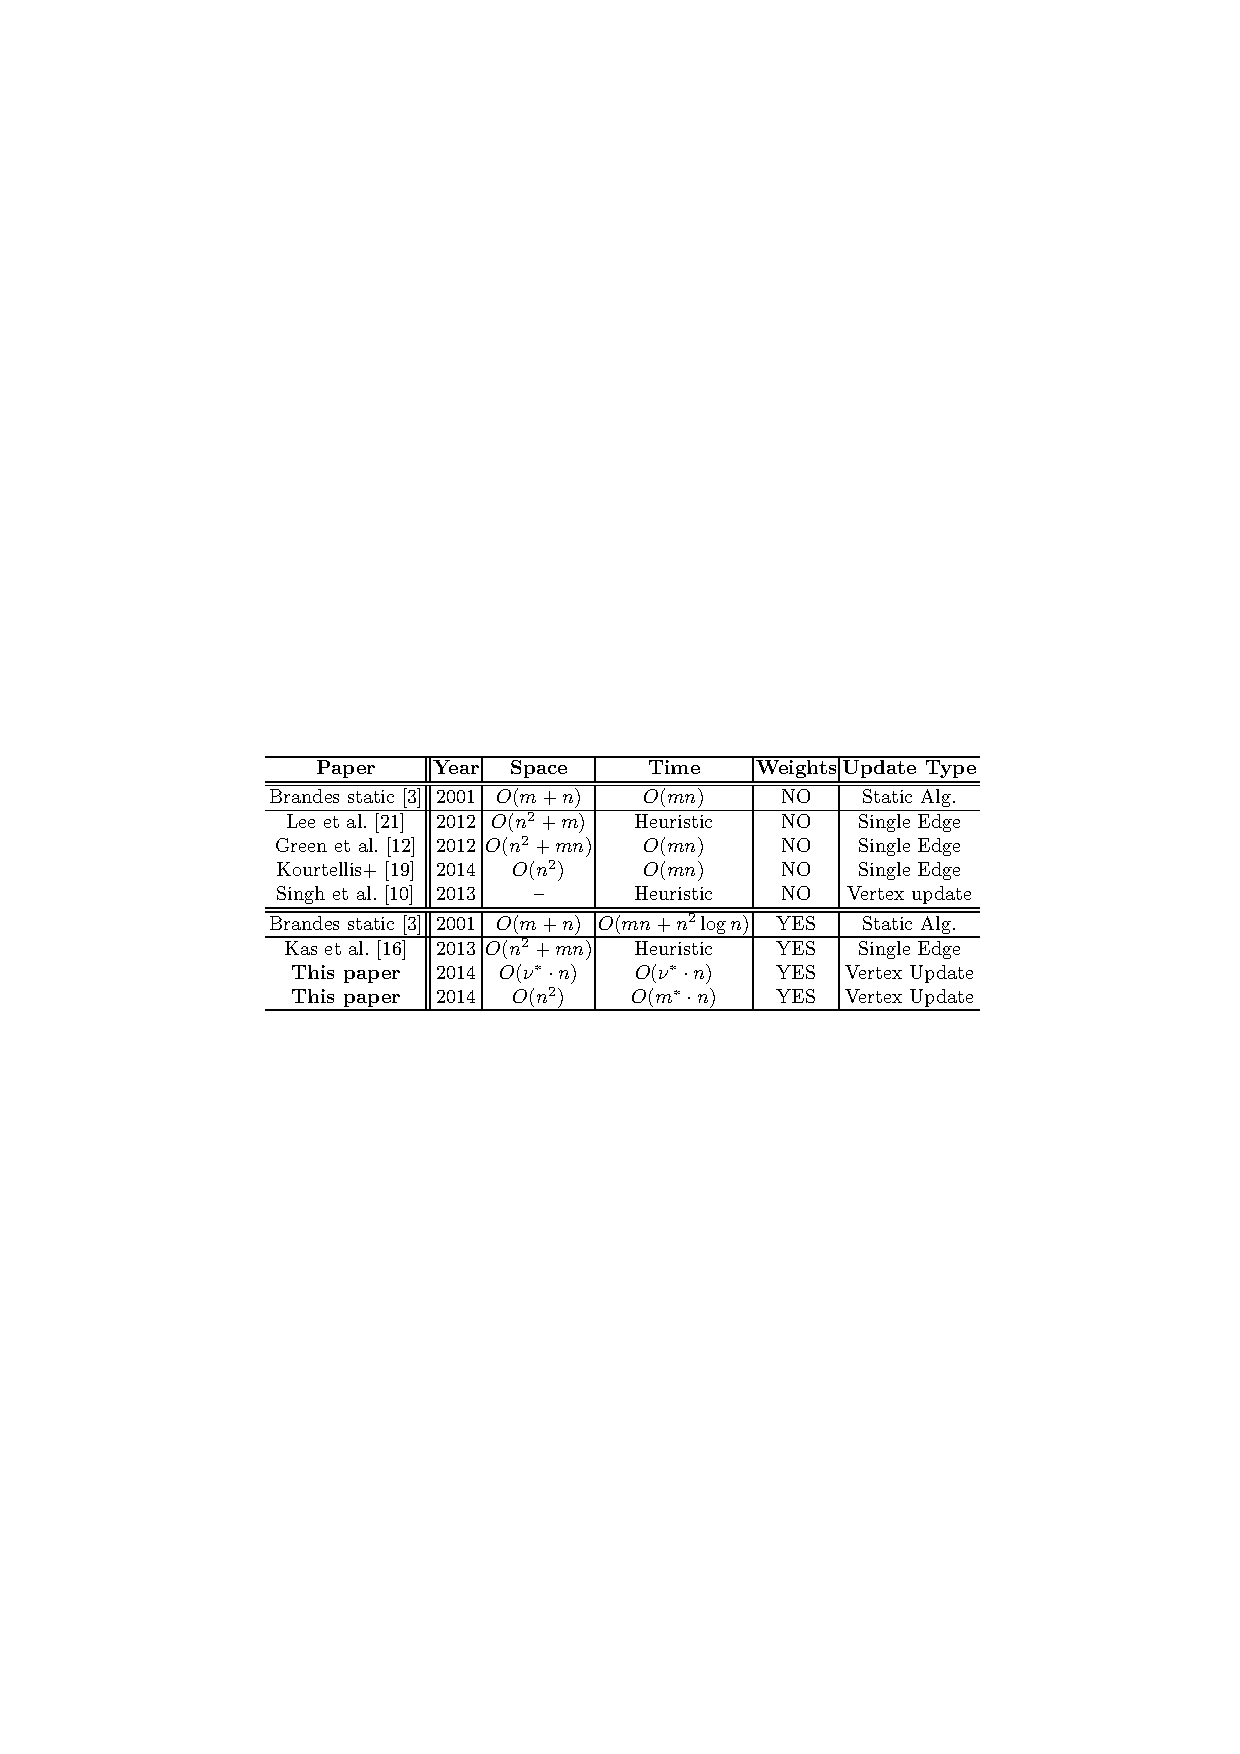
\includegraphics[width=\textwidth]{imgs/npr14-comparison}
  \end{figure}
\end{frame}


\begin{frame}
  \frametitle{Conclusions}

  \begin{itemize}
    \item Provably faster than Brandes' on weighted graphs
    \item However $m^*$ can be large in practice
    \item No experiments
    \item Hard to parallelize (need to access pairs of \spdag at a time)
    \item Still has main bottleneck of most algorithms: $O(n^2)$ memory
  \end{itemize}
\end{frame}


%% Sariyuce et al. (incremental closeness)
\begin{frame}
  \centering
  \vfill
  {\huge Incremental Algorithms for Closeness Centrality}
  \vfill
  {\Large A. E. Sar\i y\"uce, K. Kaya, E. Saule, U.~V.~\c{C}ataly\"urek }
  \vfill
  {\large IEEE BigData '13: International Conference on Big Data}
  \vfill
\end{frame}


\begin{frame}
  \frametitle{Intuition}

  \begin{itemize}
    \item Algorithm with pruning based on level difference (similar to Green et al.)
    \item Additional pruning by bi-connected decomposition (similar to QUBE)
    \item Applied to closeness centrality (still solves APSP)
    \item Reminder: closeness centrality
    \item $\displaystyle \closeness(v)=\frac{1}{\displaystyle  \sum_{u \in V} d(u,v)}$
  \end{itemize}

\end{frame}


\begin{frame}
  \frametitle{Preliminaries}

  \begin{itemize}
    \item Best static algorithm $O(nm)$ time
  \end{itemize}

  \begin{figure}[H]
    \centering
    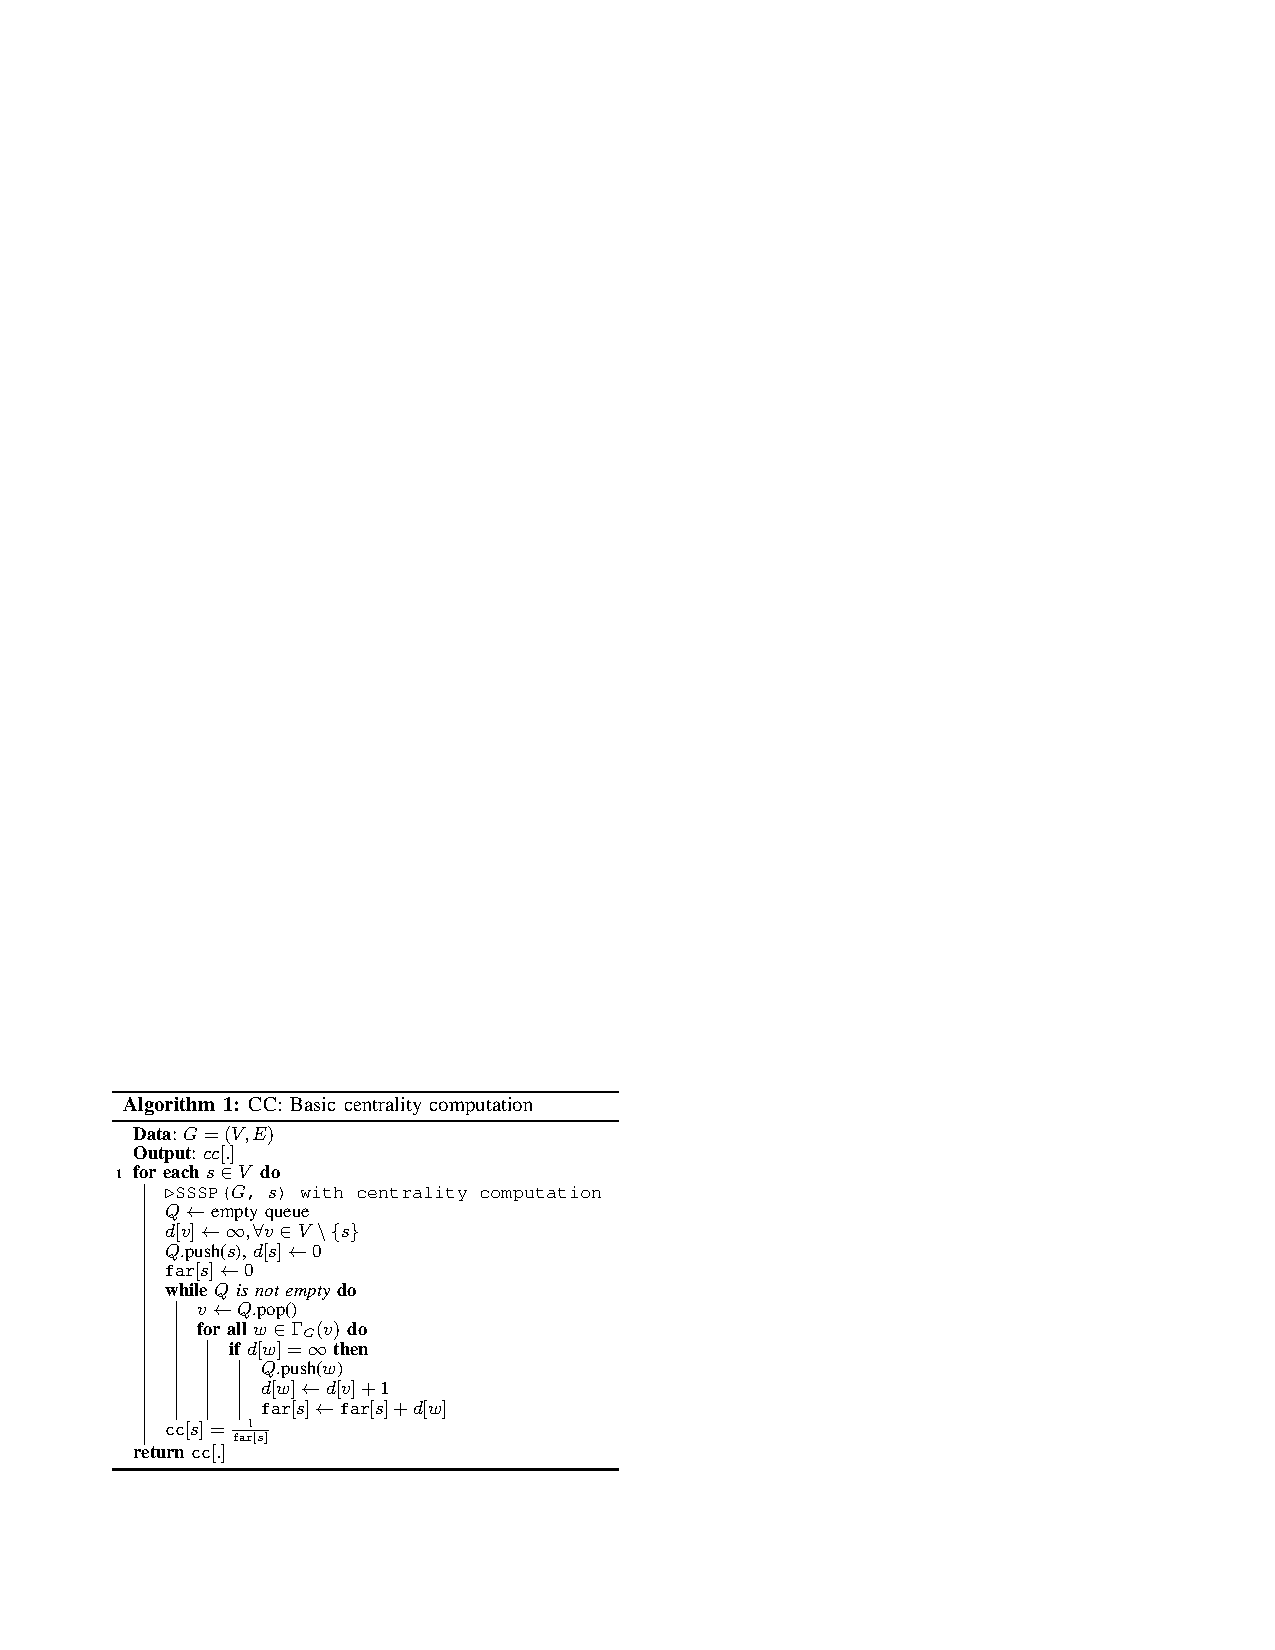
\includegraphics[width=\textwidth, height=0.7\textheight, keepaspectratio]{imgs/sksc-algo1}
  \end{figure}
\end{frame}


\begin{frame}
  \frametitle{Cases}

  \begin{figure}[H]
    \centering
    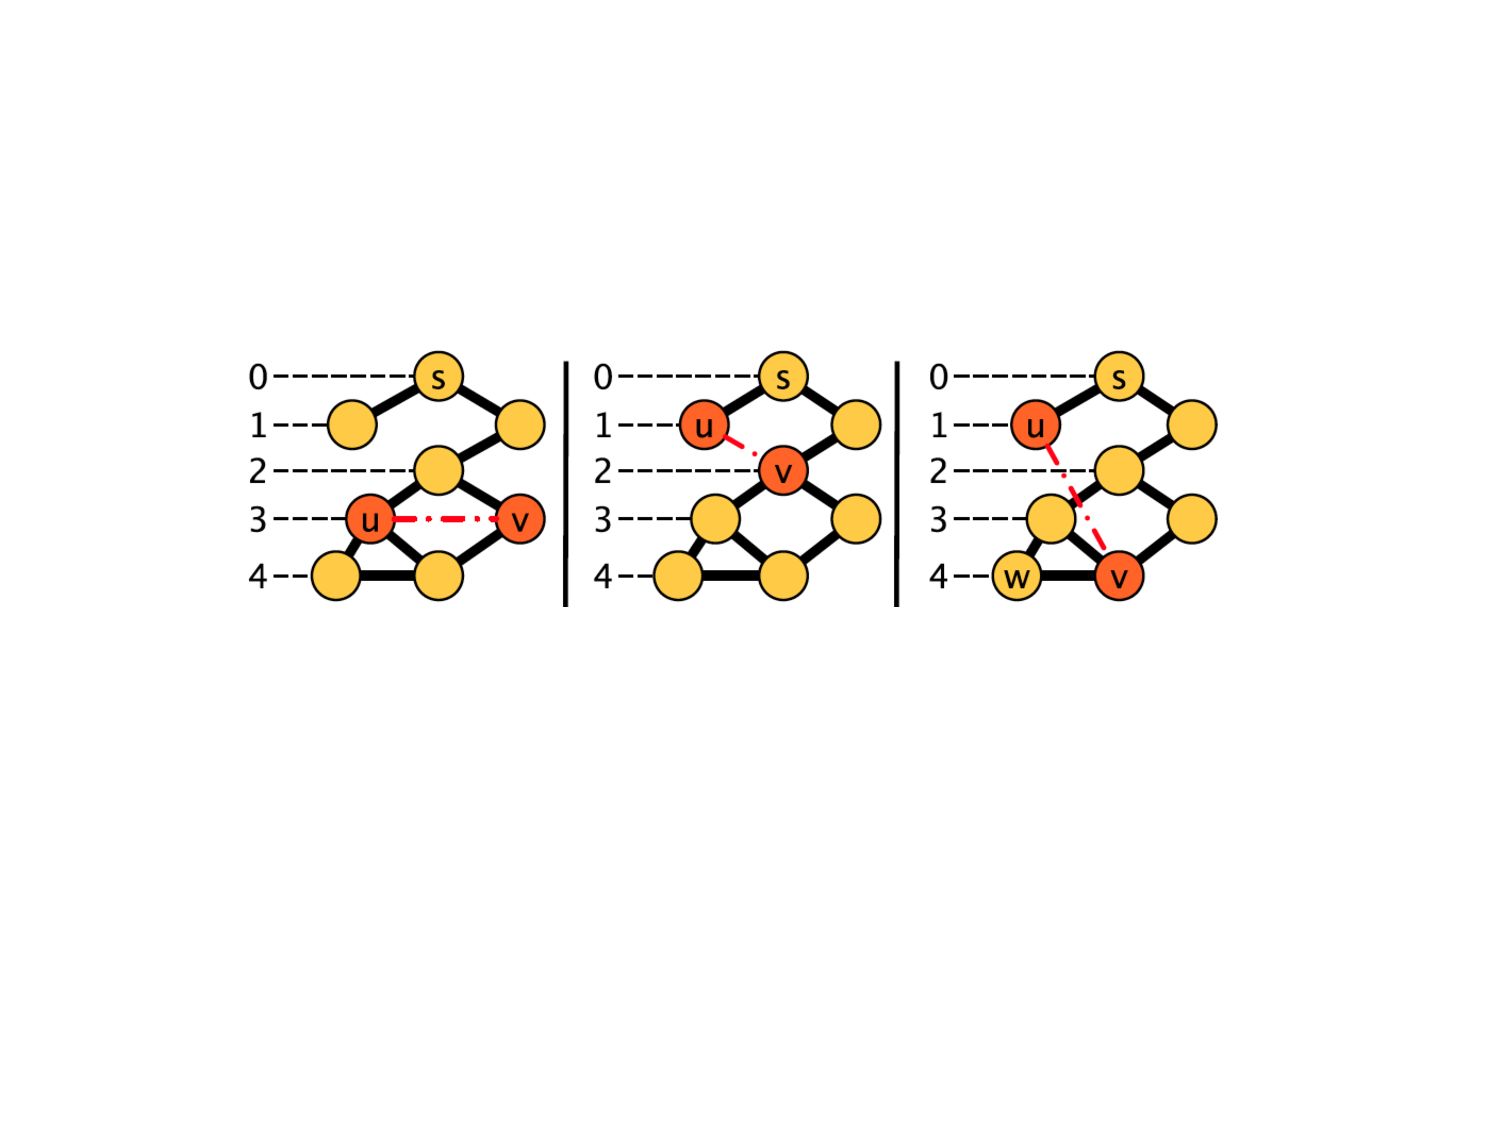
\includegraphics[width=\textwidth]{imgs/sksc-cases}
  \end{figure}

  \begin{itemize}
    \item Usual cases: $dd=0$, $dd=1$, $dd>1$
  \end{itemize}
\end{frame}


\begin{frame}
  \frametitle{Pruning - level difference}

  \begin{figure}[H]
    \centering
    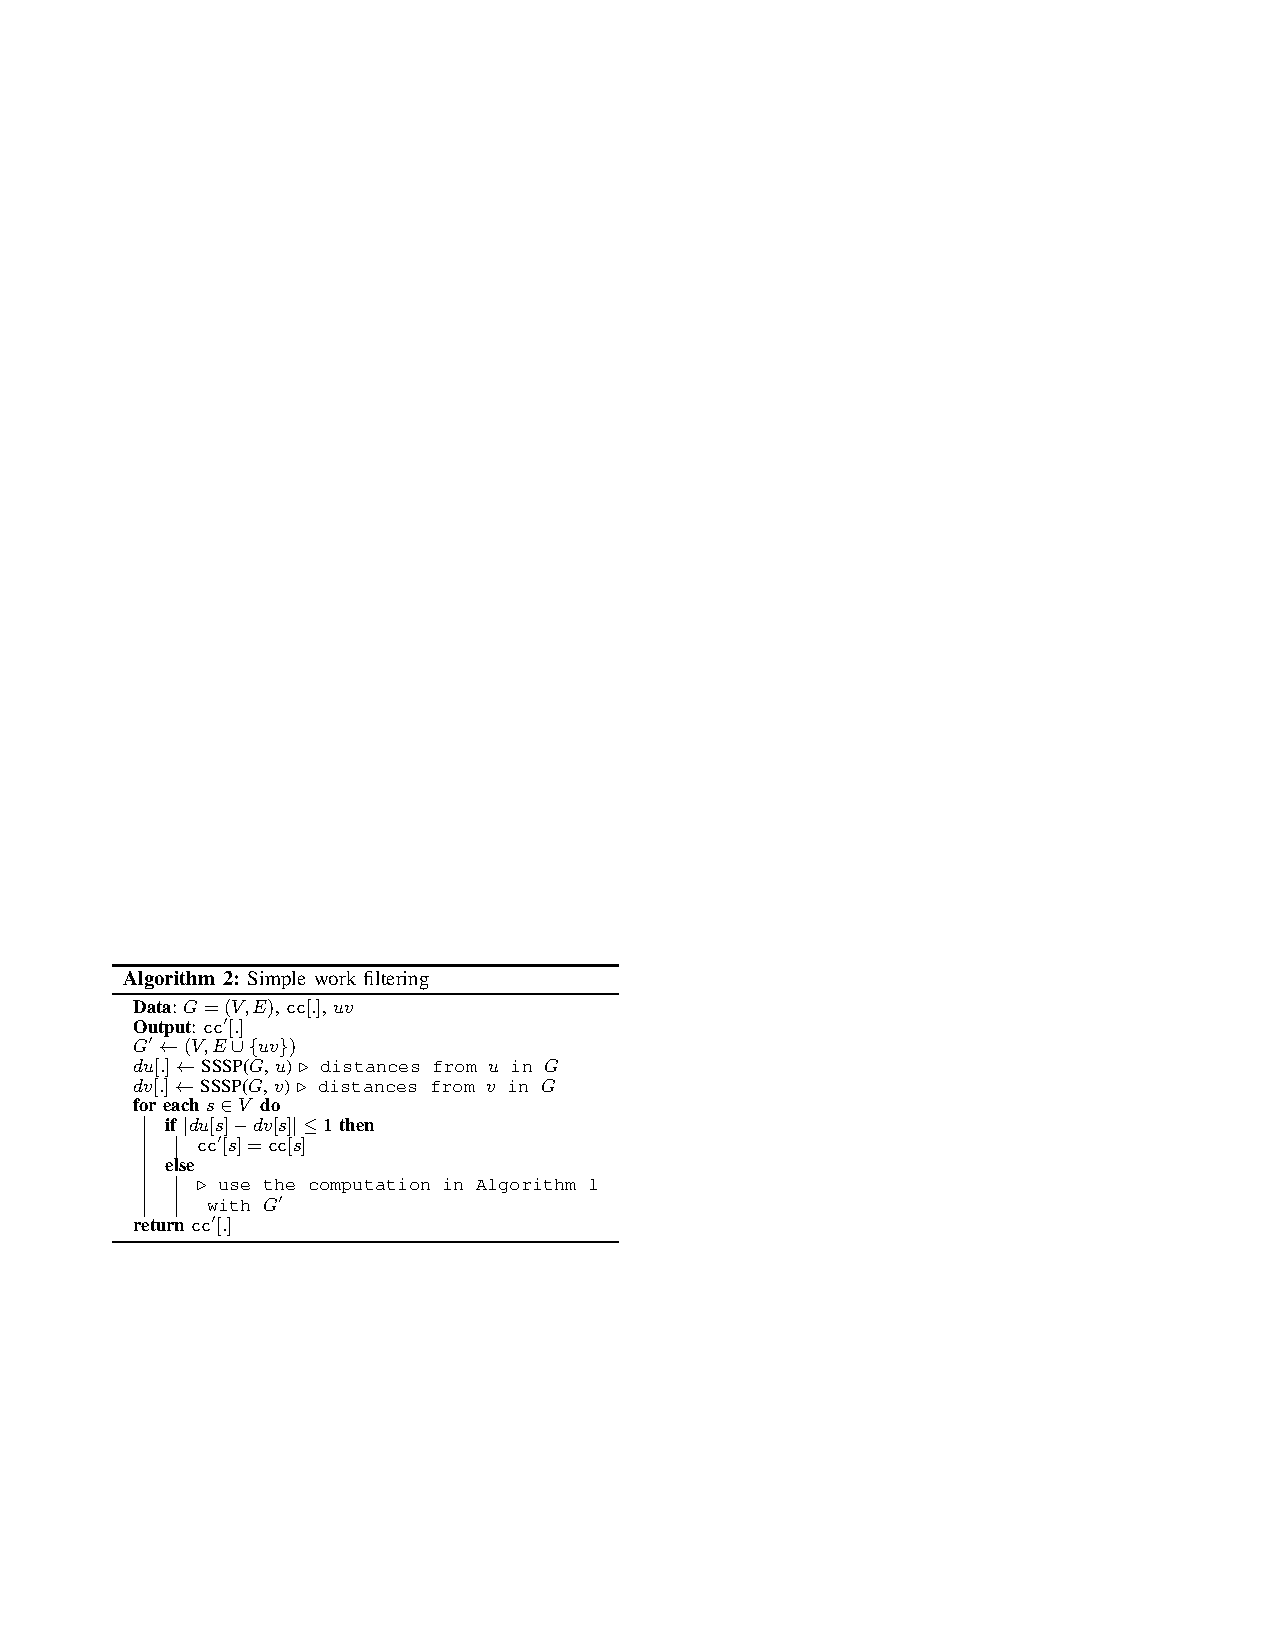
\includegraphics[width=\textwidth, height=0.7\textheight, keepaspectratio]{imgs/sksc-algo2}
  \end{figure}
\end{frame}


\begin{frame}
  \frametitle{Pruning - biconnected components}

  \begin{figure}[H]
    \centering
    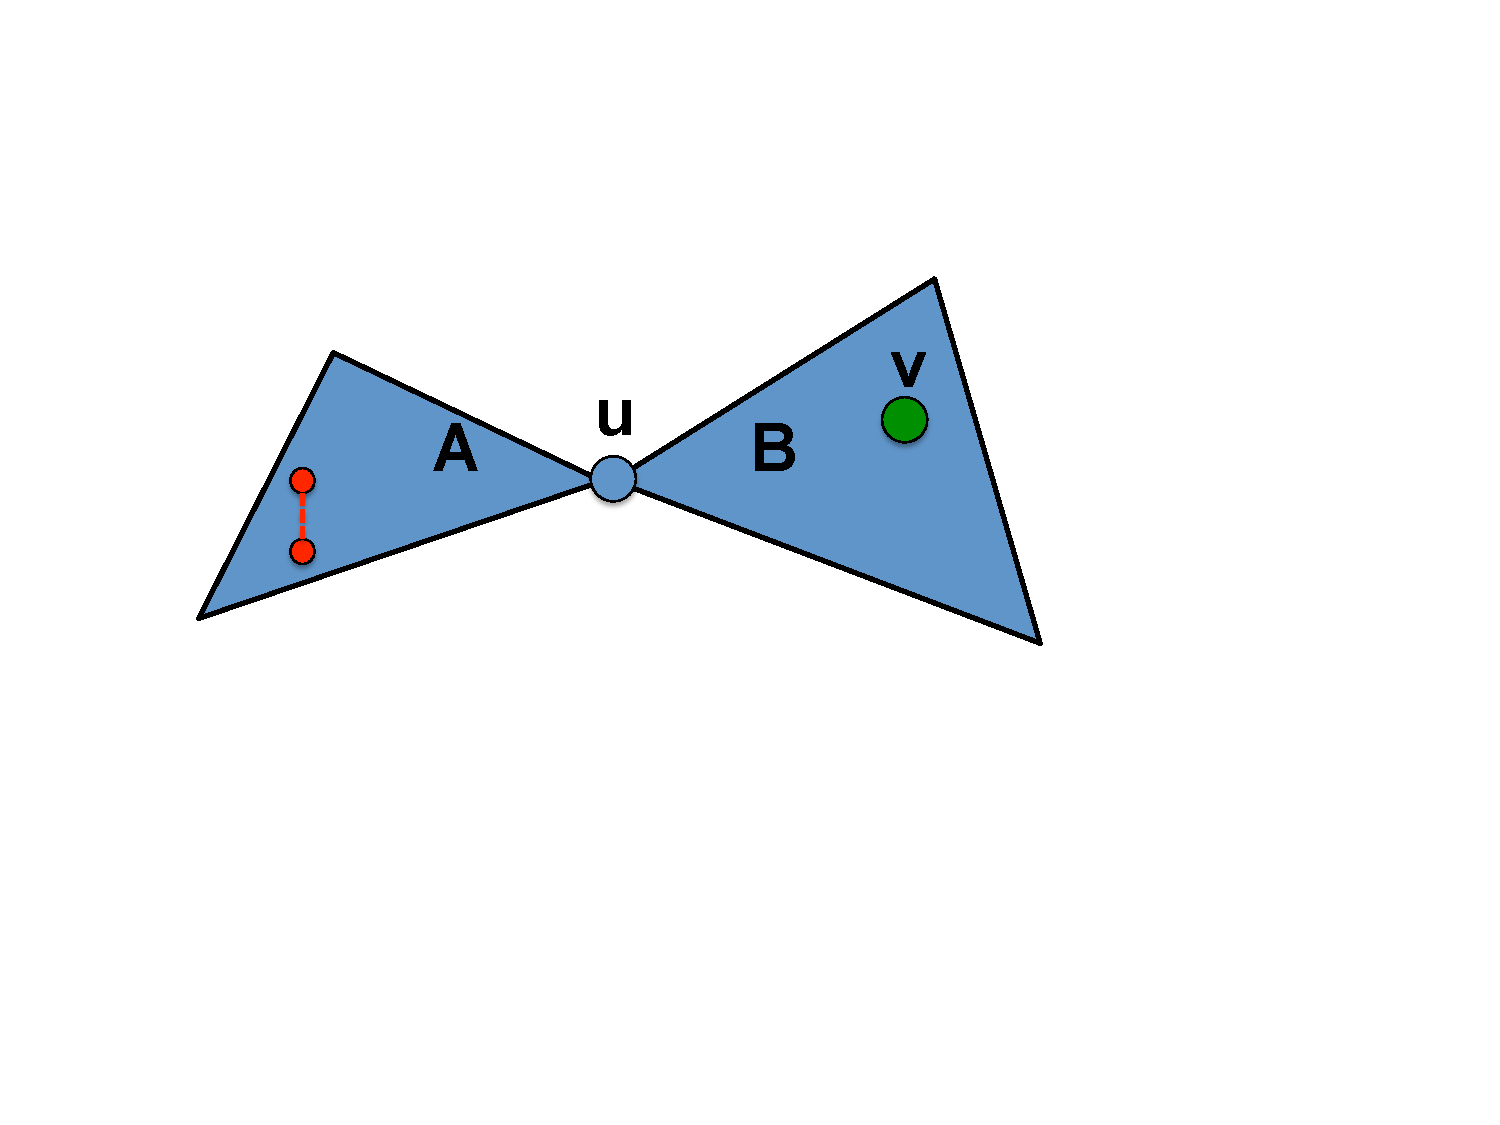
\includegraphics[width=\textwidth, height=0.5\textheight, keepaspectratio]{imgs/sksc-biconnected}
  \end{figure}

  \begin{itemize}
    \item If graph has articulation points
    \item Change in $A$ can change closeness of any vertex in $B$
    \item It is enough to compute change for $u$ (constant factor is added for the rest of $B$)
  \end{itemize}
\end{frame}


\begin{frame}
  \frametitle{Maintaining biconnected decomposition}

  \begin{figure}[H]
    \centering
    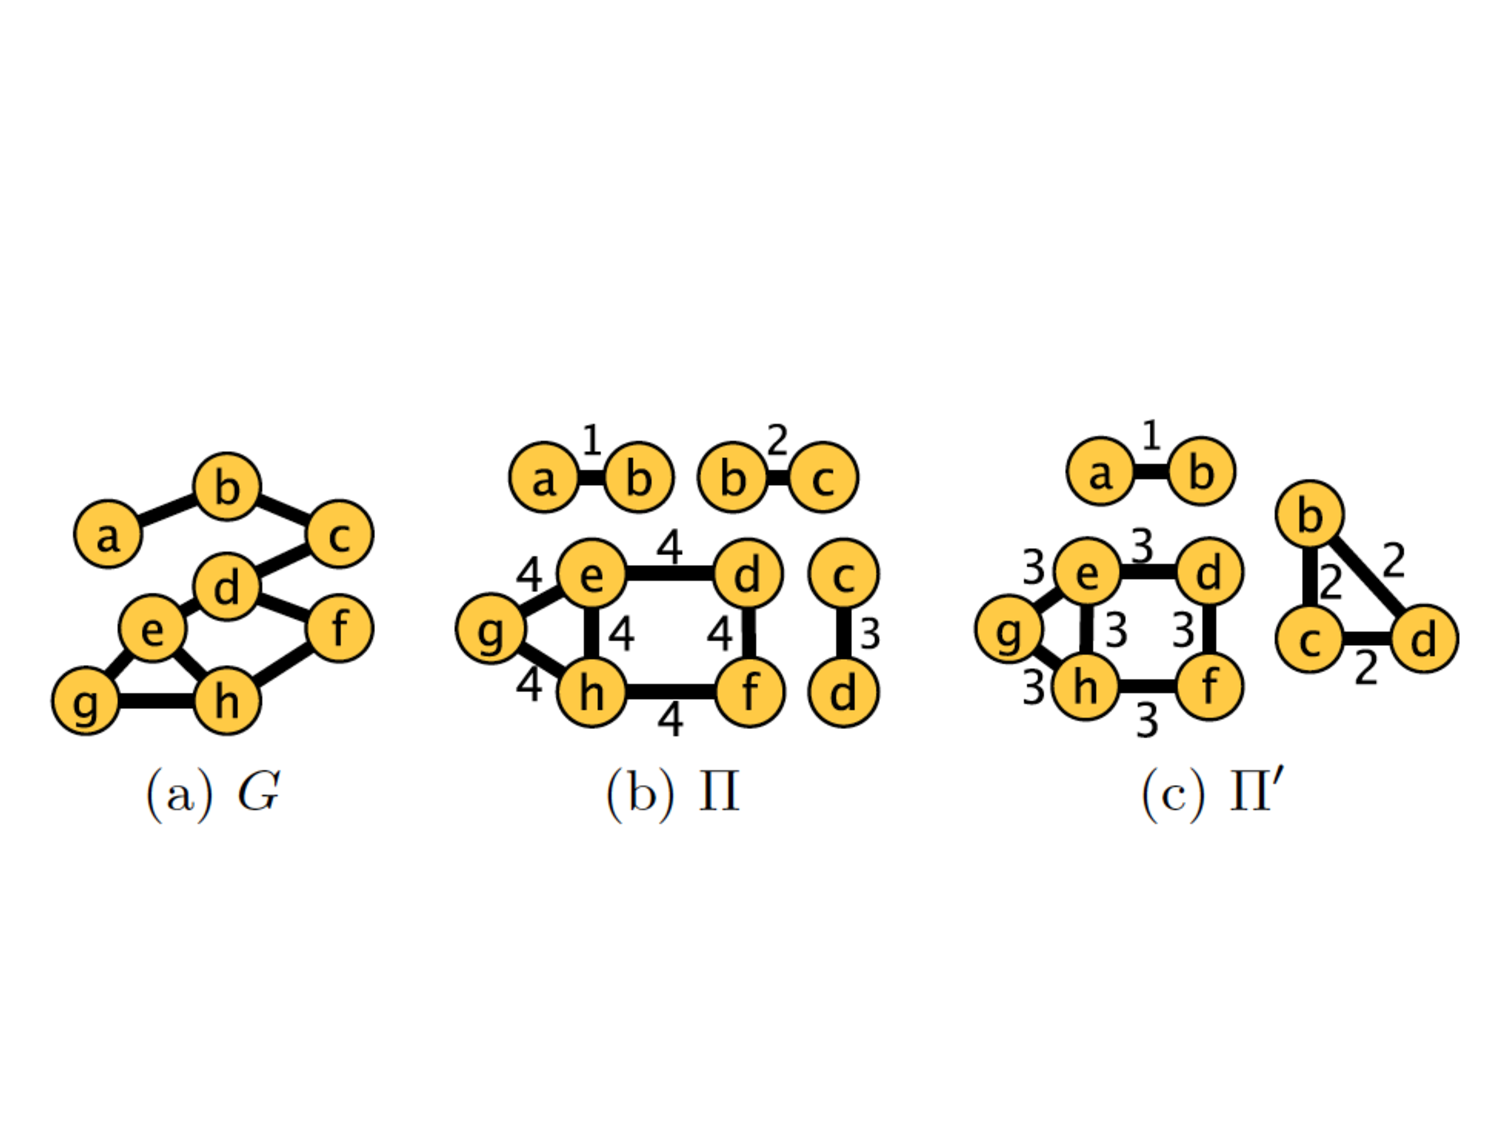
\includegraphics[width=\textwidth, height=0.5\textheight, keepaspectratio]{imgs/sksc-bidecomp}
  \end{figure}

  \begin{itemize}
    \item Assume edge $(b,d)$ added
    \item Similar to QUBE
  \end{itemize}
\end{frame}


\begin{frame}
  \frametitle{\sssp hybridization}

  \begin{itemize}
    \item BFS can be performed in two ways
    \item \emph{Top-down:} process vertices at distance $d$ to find vertices at distance $d+1$
    \item \emph{Bottom-up:} after vertices at distance $d$ are found, process all unprocessed vertices to see if they are neighbors of the frontier
    \item Top-down is better for initial rounds, bottom-up better for final rounds
    \item Hybridization: use best option at each round
  \end{itemize}
\end{frame}


\begin{frame}
  \frametitle{Fraction of cases}

  \begin{figure}[H]
    \centering
    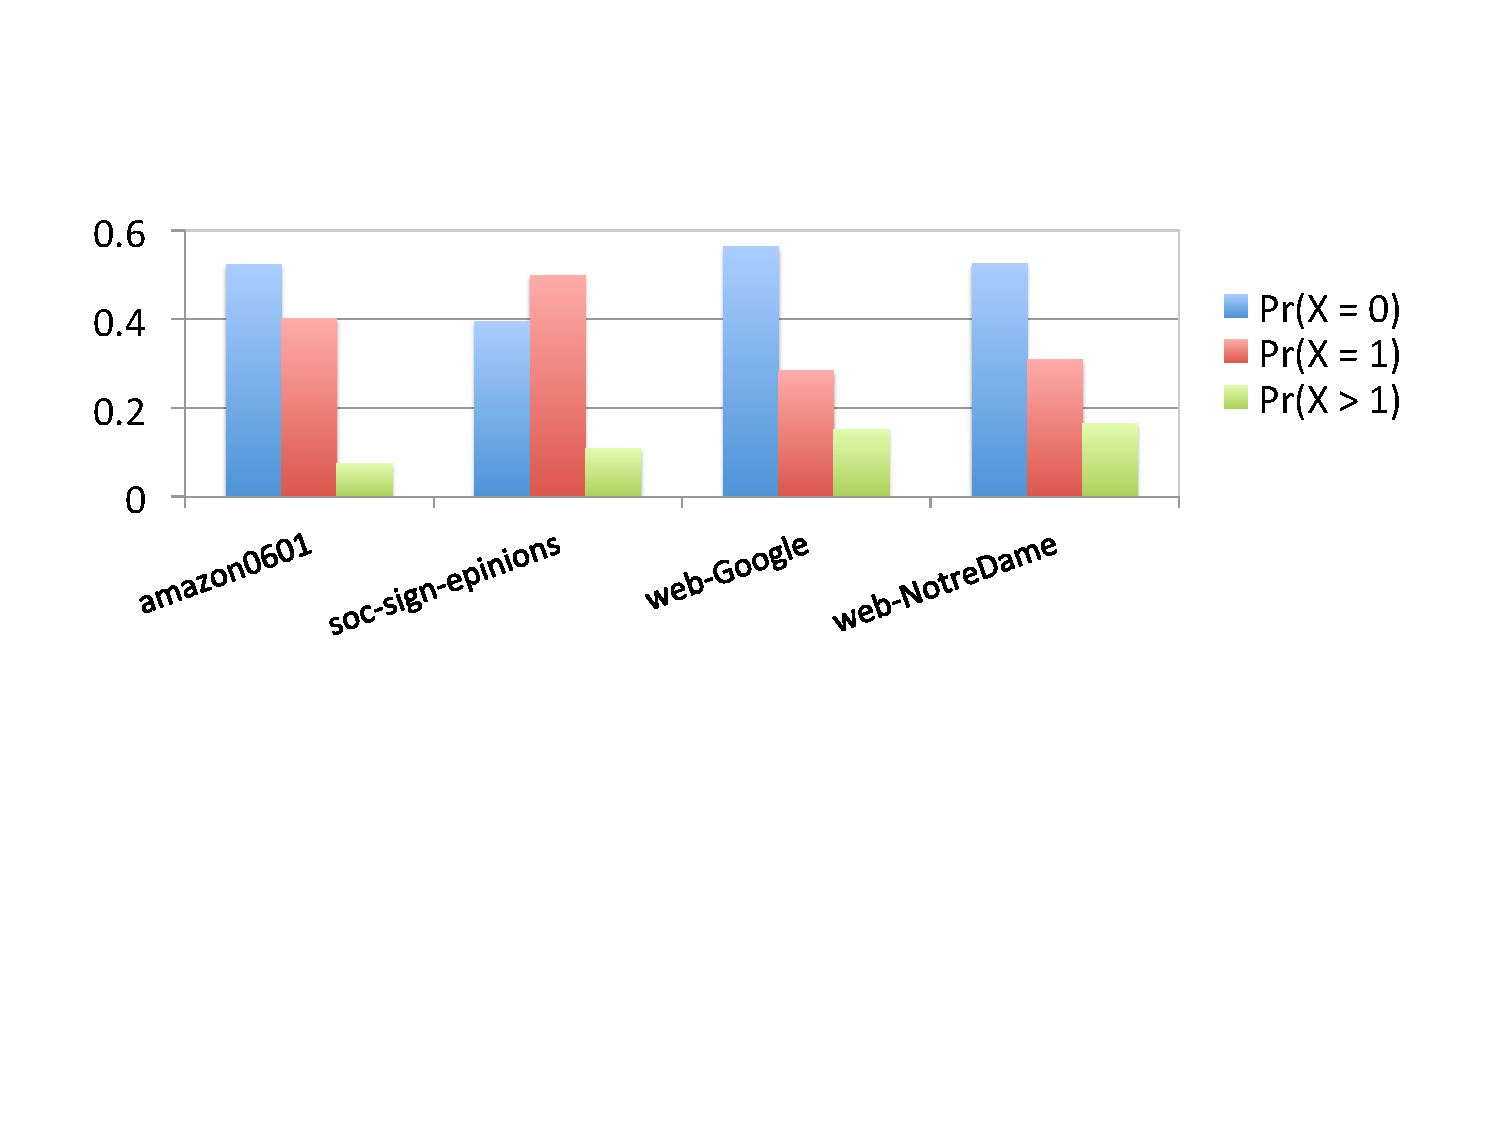
\includegraphics[width=\textwidth, height=0.5\textheight, keepaspectratio]{imgs/sksc-results1}
  \end{figure}

  \begin{itemize}
    \item Probability distribution for level difference $dd$
    \item Most edges are easy cases
  \end{itemize}
\end{frame}

\begin{frame}
  \frametitle{Speedup}

  \begin{figure}[H]
    \centering
    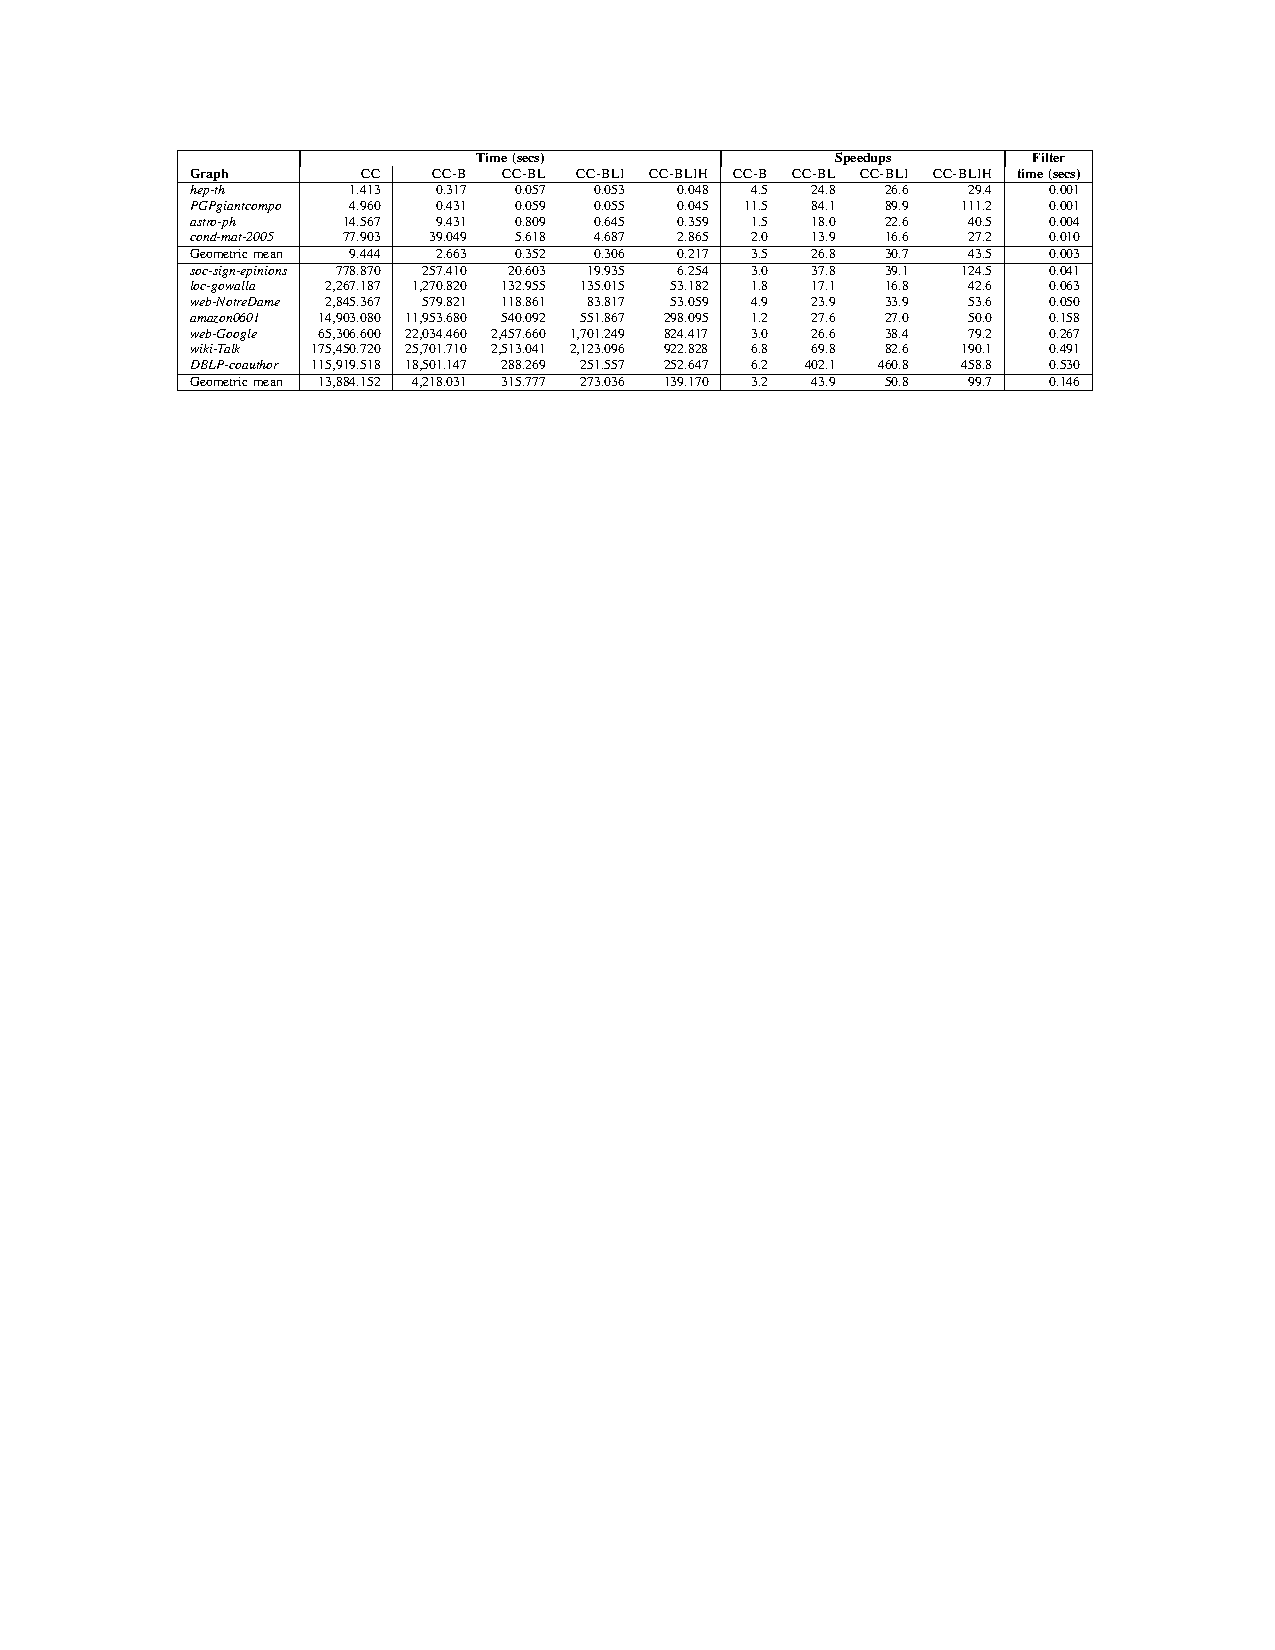
\includegraphics[width=\textwidth, height=0.5\textheight, keepaspectratio]{imgs/sksc-results2}
  \end{figure}

  \begin{itemize}
    \item Speedup of 2 orders of magnitude
    \item Mostly due to level pruning
    \item Biconnected decomposition and hybridization also give good speedups
  \end{itemize}
\end{frame}


%% Kourtellis et al.
\begin{frame}
  \centering
  \vfill
  {\huge Scalable Online Betweenness Centrality in Evolving Graphs}
  \vfill
  {\Large N. Kourtellis, G. De-Francisci-Morales, F. Bonchi}
  \vfill
  {\large TKDE: IEEE Transactions on Knowledge and Data Engineering (2015)}
  \frametitle{Scalable Online Betweenness Centrality in Evolving Graphs}
  \vfill
\end{frame}


\begin{frame}
  \frametitle{Intuition}

  \begin{itemize}
    \item Incremental, exact, space-efficient, out-of-core, parallel version of Brandes'
    \item Handles edge addition and removal
    \item Vertex and edge betweenness
    \item Scalable to graphs with millions of vertices
  \end{itemize}

\end{frame}


\begin{frame}
  \frametitle{Algorithm}

  \begin{itemize}
    \item Run a modified Brandes' on the initial graph
    \item Keep track of \dist, \paths, \dep in a \spdag (no \pred)
    \item On edge update, adjust the \spdag and update \betw
  \end{itemize}

  \begin{figure}[t]
    \centering
    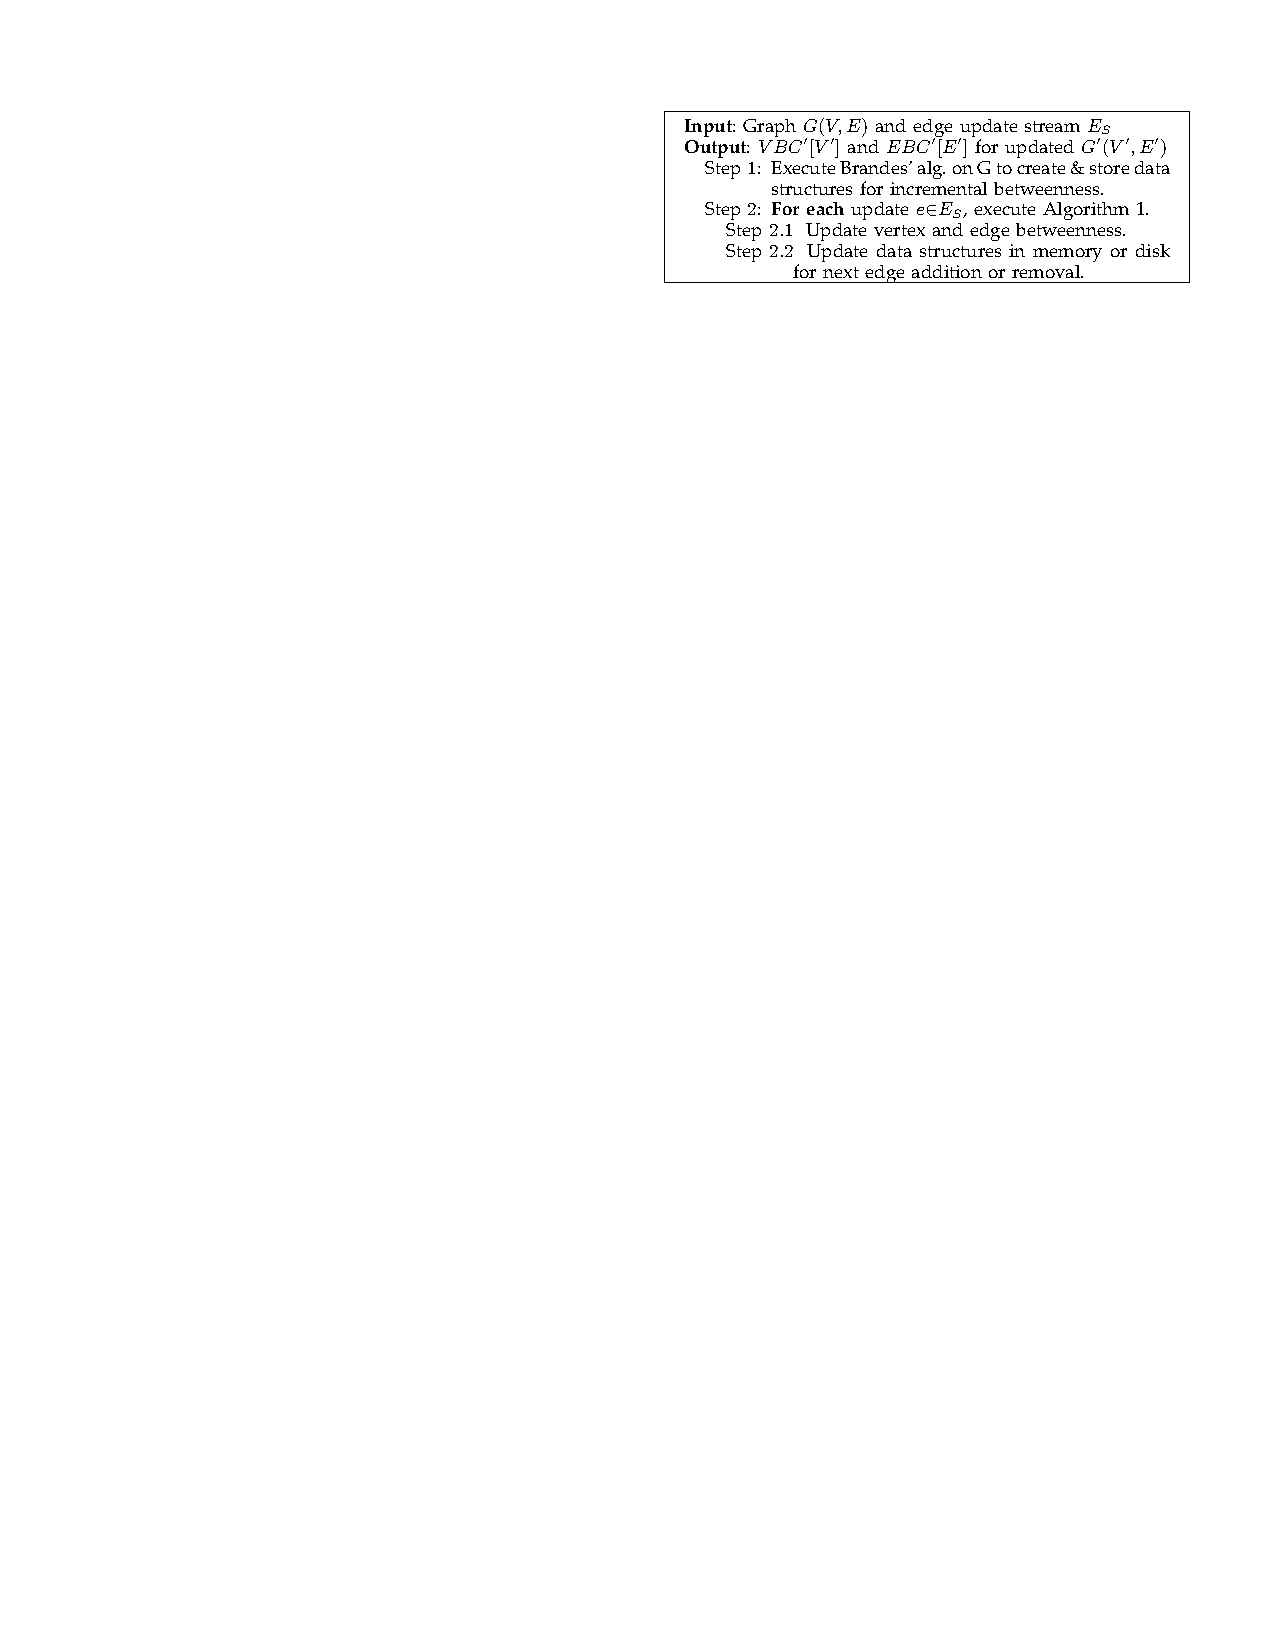
\includegraphics[width=\textwidth, height=0.6\textheight, keepaspectratio]{imgs/kdb-algo}
  \end{figure}

\end{frame}


\begin{frame}
  \frametitle{Data structure}

  \begin{itemize}
    \item $\spdag_s$ for each source $s \in V$
    \item \spdag contains \dist, \paths, \dep for each other vertex $t \in V$
    \item No predecessors \pred, re-scan neighbors and use \dist to find them
      \begin{itemize}
        \item Save memory - space complexity $O(n^2)$
        \item Fixed size data structure - efficient out-of-core management
        \item Same time complexity $O(nm)$ - in practice, makes the algorithm faster
      \end{itemize}
  \end{itemize}

\end{frame}


\begin{frame}
  \frametitle{Pivot}

  \begin{itemize}
    \item When adding or removing an edge, consider $dd = |d_{su} - d_{sv}|$
    \item Three cases: $dd=0$, $dd=1$, $dd>1$ (analogous to Green et al.)
    \item Last case $dd>1$ hardest - structural changes in \spdag
    \item Find \emph{pivots} to discover structural changes
  \end{itemize}

  \begin{definition}[Pivot]
    Let $s$ be the current source, let $\dist$ and $\dist'$ be the distance before and after an update, respectively, we define \emph{pivot} a vertex $p \mid \dist(s,p) = \dist'(s,p) \wedge \exists \, w \in \neighbors(p)$$: \dist(s,w)$$\neq$$\dist'(s,w)$.
  \end{definition}

  \begin{itemize}
    \item Pivots' distance unchanged $\rightarrow$ use as starting points to correct distances
  \end{itemize}

\end{frame}


\begin{frame}
  \frametitle{Finding pivots}

  \begin{itemize}
    \item Addition - pivots in sub-dag rooted in $u_L = v$
    \item vertices moved closer must be reachable from $u_L$
    \item Can be found during exploration while fixing \paths
  \end{itemize}
  \begin{itemize}
    \item Removal - pivots may be anywhere
    \item Need one exploration to find them
    \item Need separate exploration from found pivots to correct distances
  \end{itemize}

  \begin{figure}[t]
    \centering
    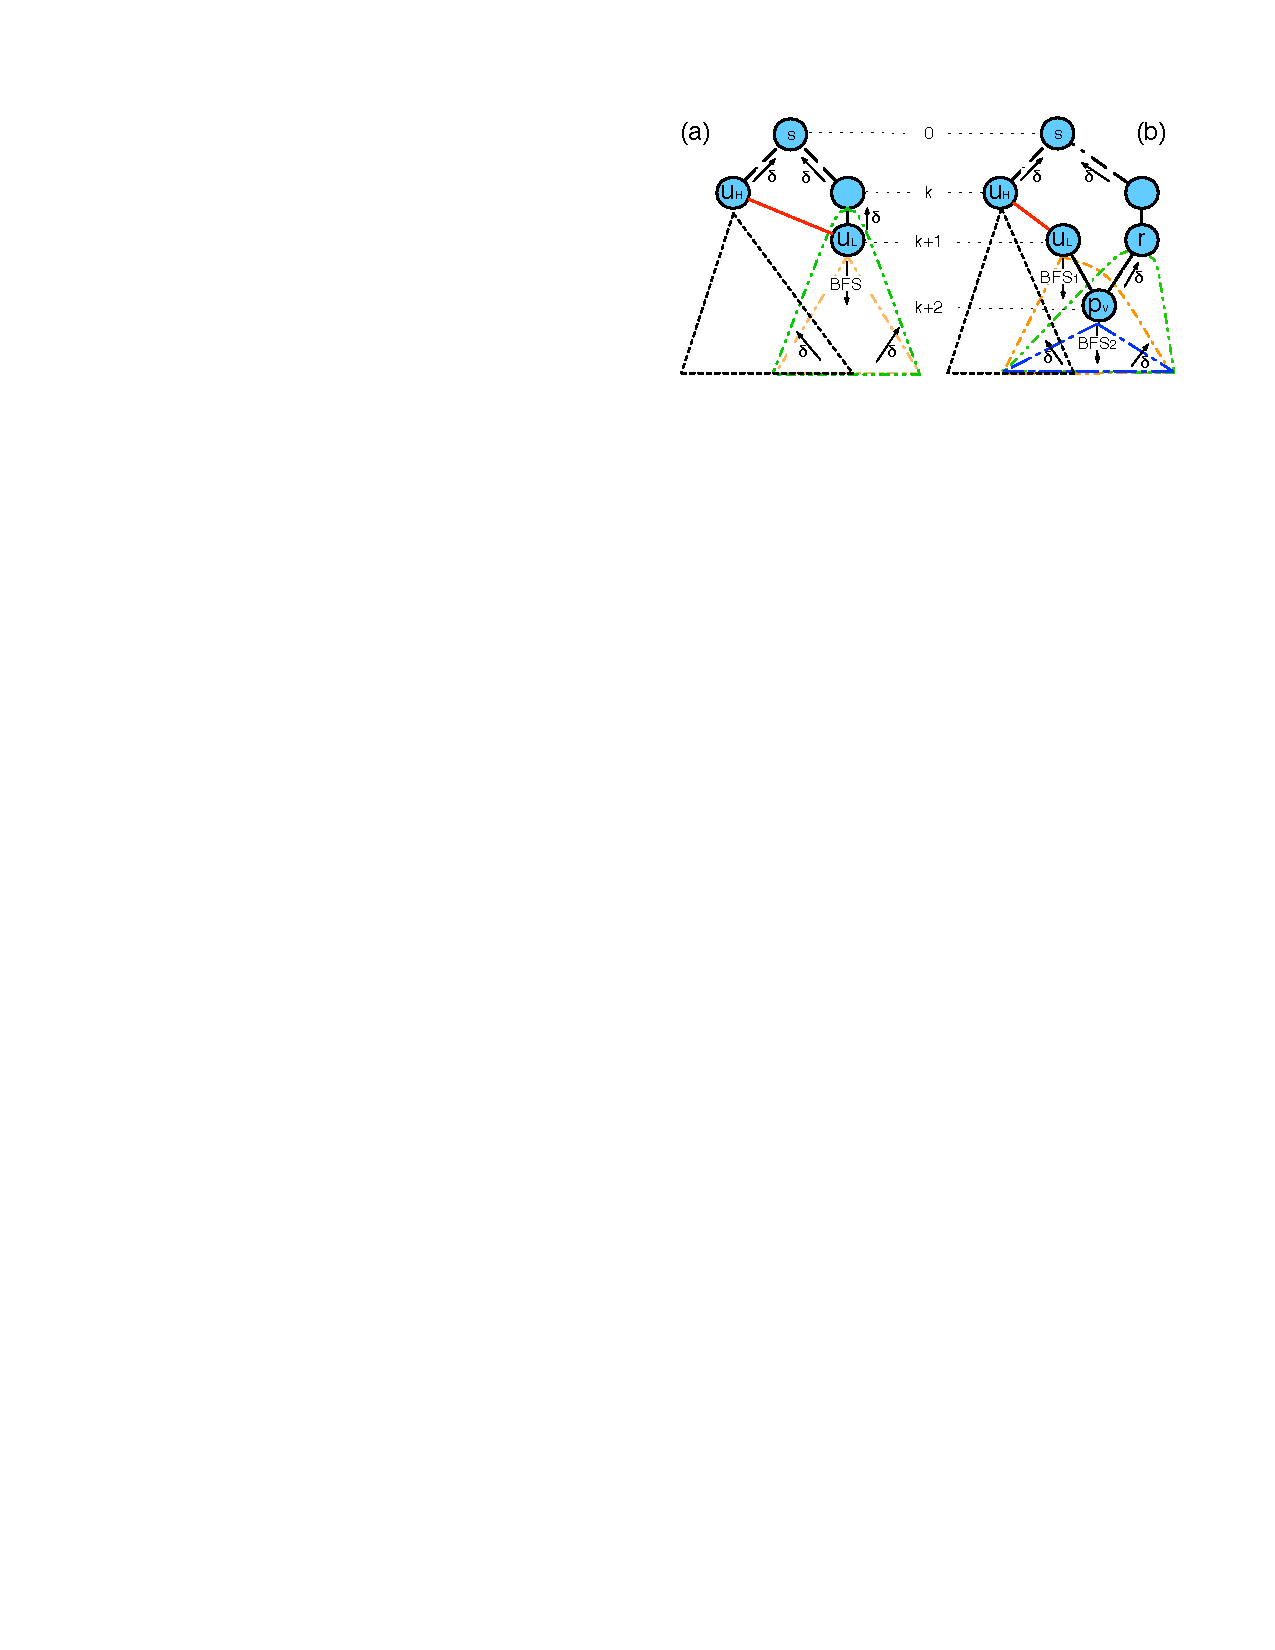
\includegraphics[width=\textwidth, height=0.5\textheight, keepaspectratio]{imgs/kdb-bfs}
  \end{figure}

\end{frame}


\begin{frame}
  \frametitle{Structural changes}

  \begin{figure}[t]
    \centering
    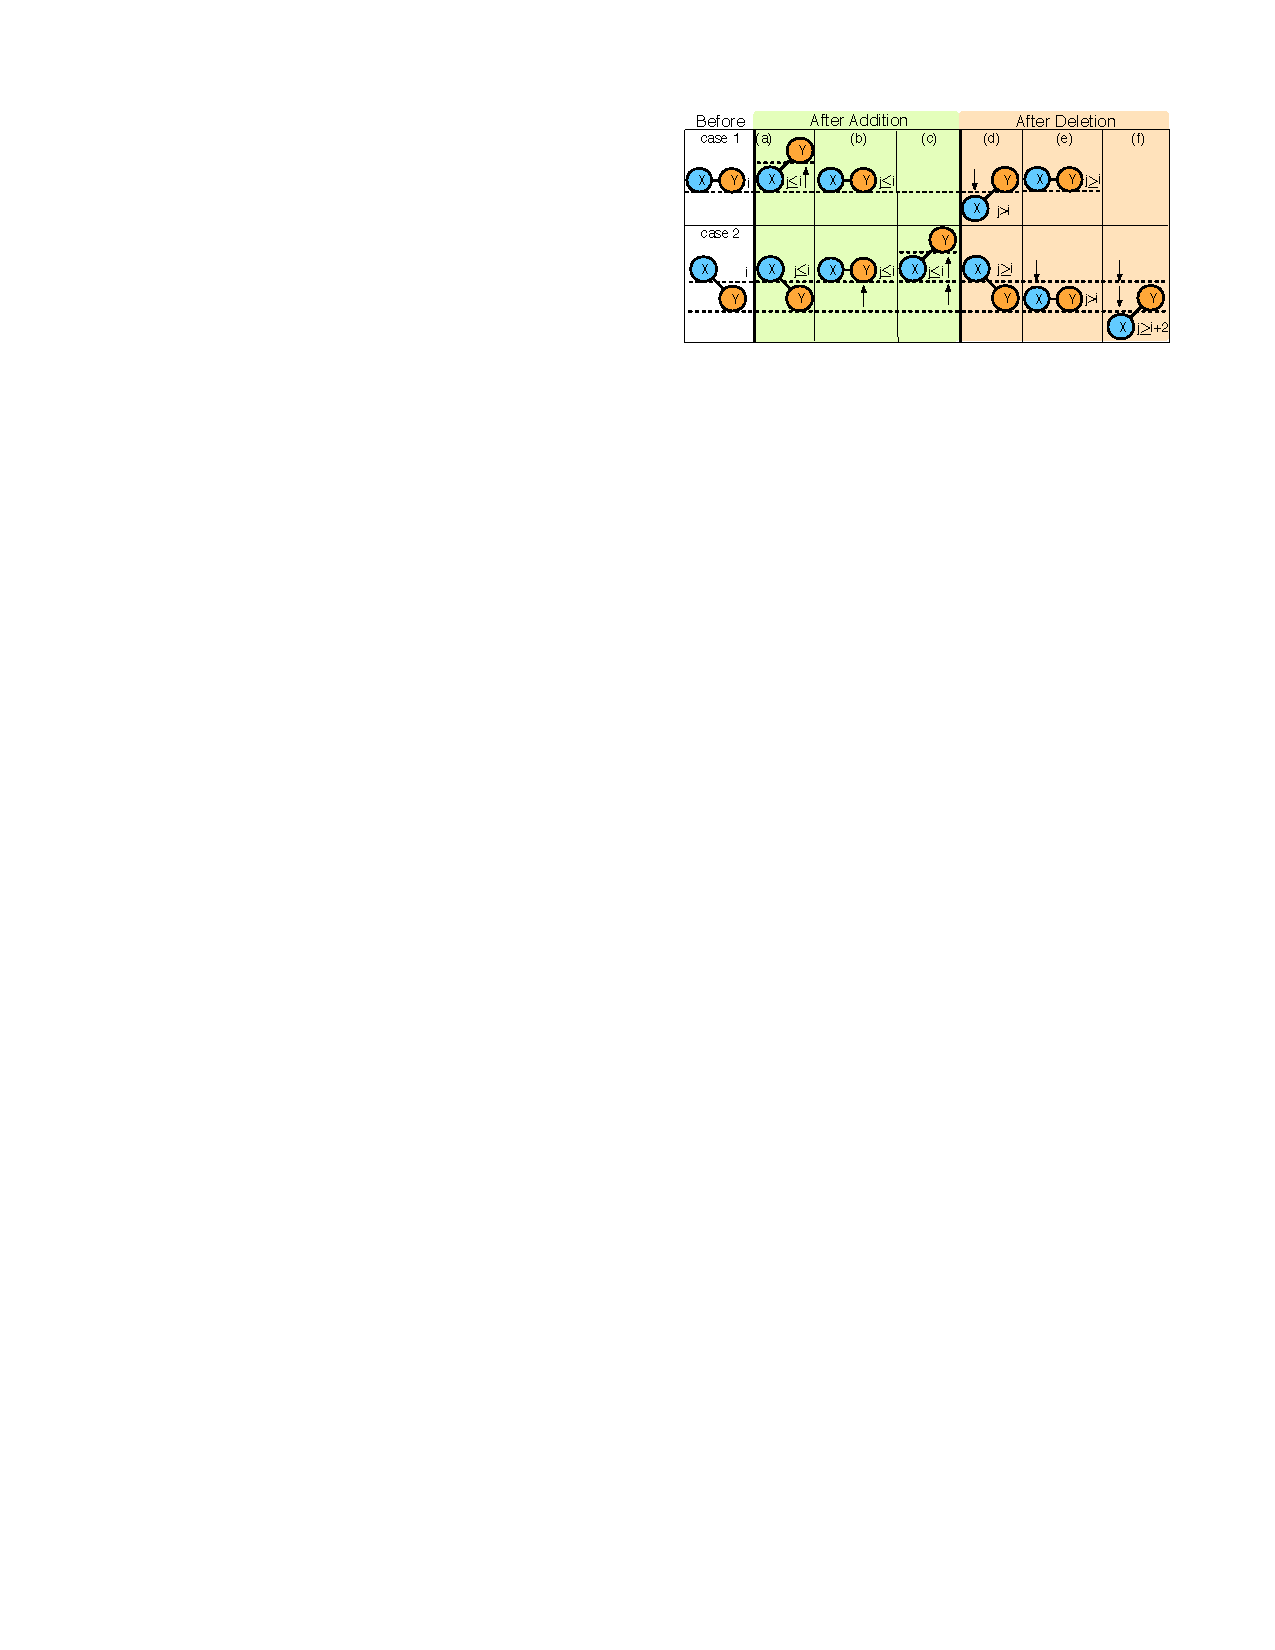
\includegraphics[width=\textwidth, height=0.5\textheight, keepaspectratio]{imgs/kdb-cases}
  \end{figure}

  \begin{itemize}
    \item Consider $x \in \neighbors(y)$, $x$ can either be a sibling or a predecessor of $y$
    \item Each case requires slightly different combination of corrections for \dist, \paths, \dep
    \item $y$ is pivot in 1d, 2e, 2f
    \item Removal for case 1d can be optimized (pivot $y$ is sibling of $x$)
  \end{itemize}

\end{frame}


\begin{frame}
  \frametitle{Scalability}

  \begin{itemize}
    \item Out-of-core - stream \spdag from disk
      \begin{itemize}
        \item In-place update on disk to minimize writes
      \end{itemize}
    \item Columnar storage for \dist, \paths, \dep
      \begin{itemize}
        \item Read only \dist, skip rest if $dd=0$
      \end{itemize}
    \item Parallelization - coarse grained over $s$
      \begin{itemize}
        \item Implementation in MapReduce
        \item Amenable to Apache Storm/Flink/Spark
      \end{itemize}
  \end{itemize}

\end{frame}


\begin{frame}
  \frametitle{Results}

  \begin{figure}[t]
    \centering
    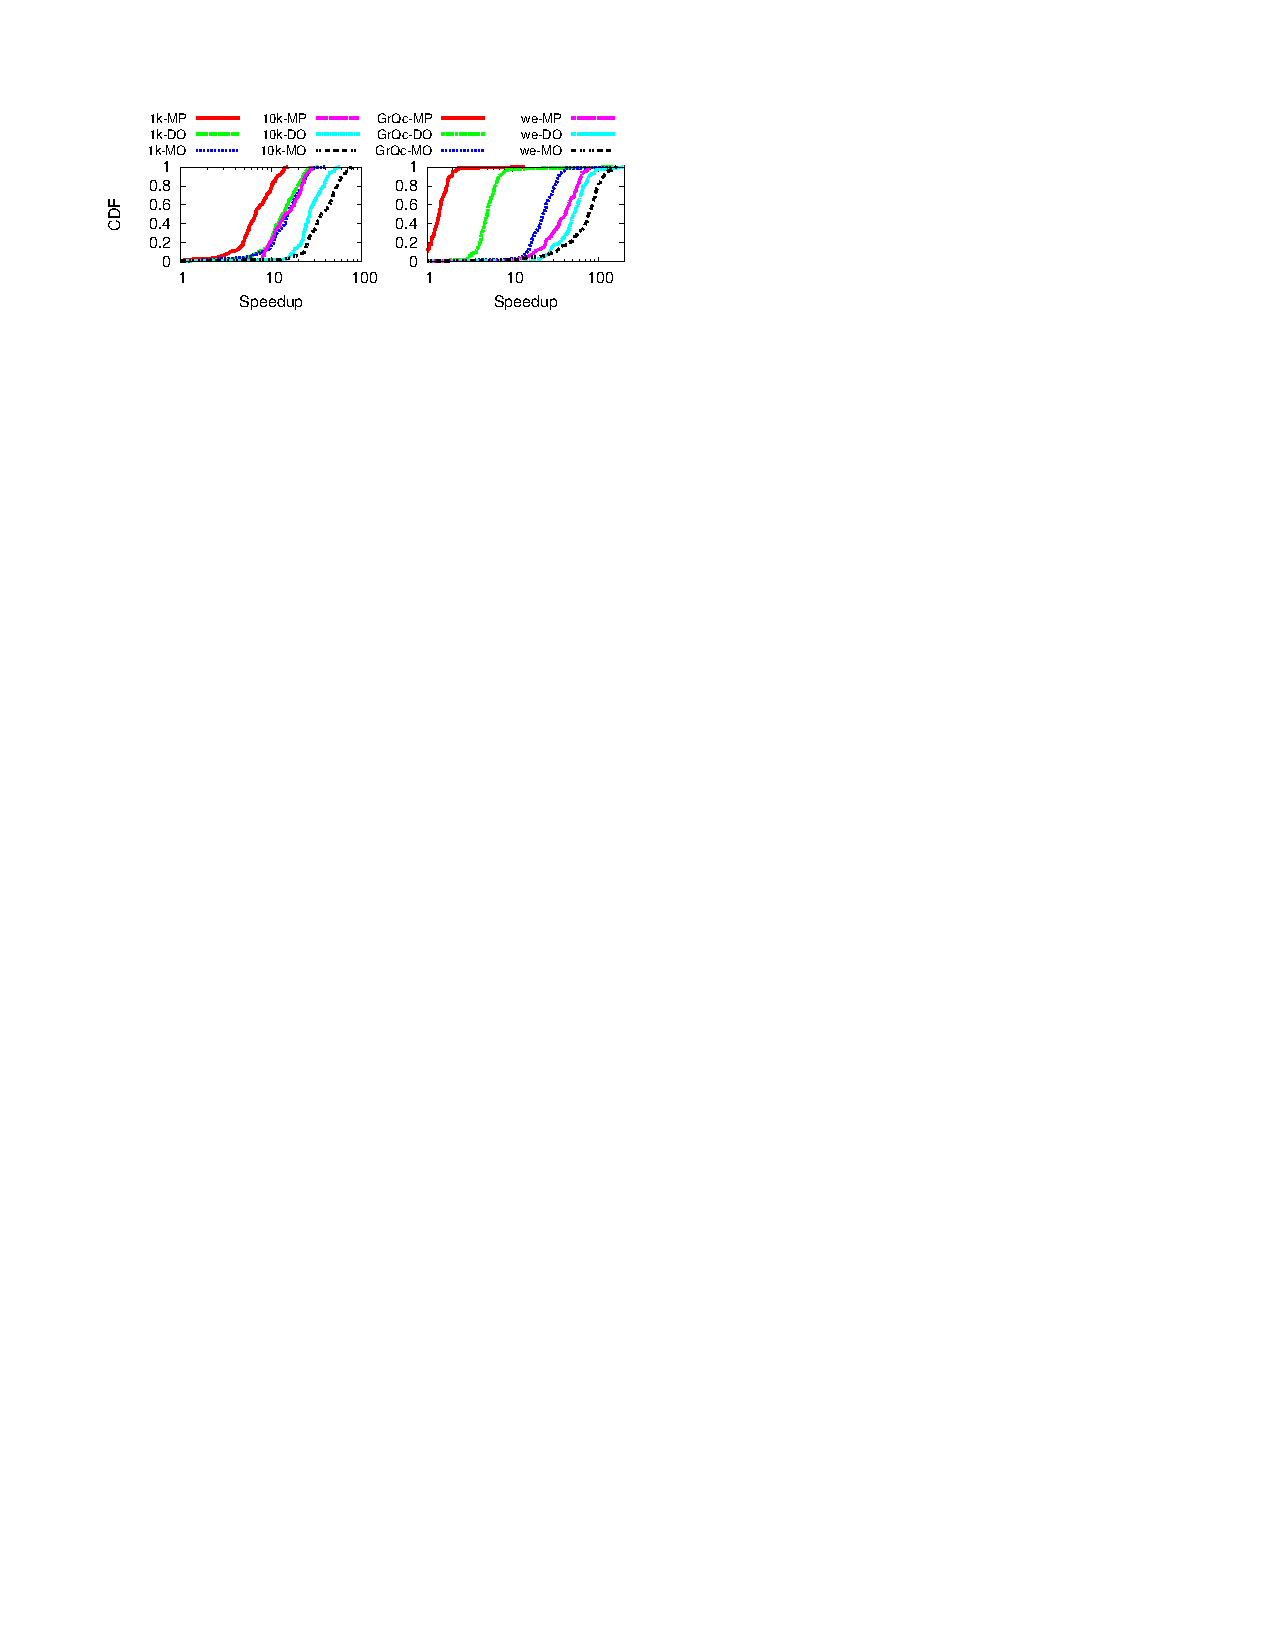
\includegraphics[width=\textwidth, height=0.6\textheight, keepaspectratio]{imgs/kdb-results1}
    \caption{Speedup over Brandes' on synthetic and real graphs ($n = 10k$)}
  \end{figure}

  \begin{itemize}
    \item In-memory (M-) version faster than out-of-core (D-)
    \item Without predecessor (-O) always faster than with predecessors (-P)
  \end{itemize}

\end{frame}


\begin{frame}
  \frametitle{Results}

  \begin{figure}[t]
    \centering
    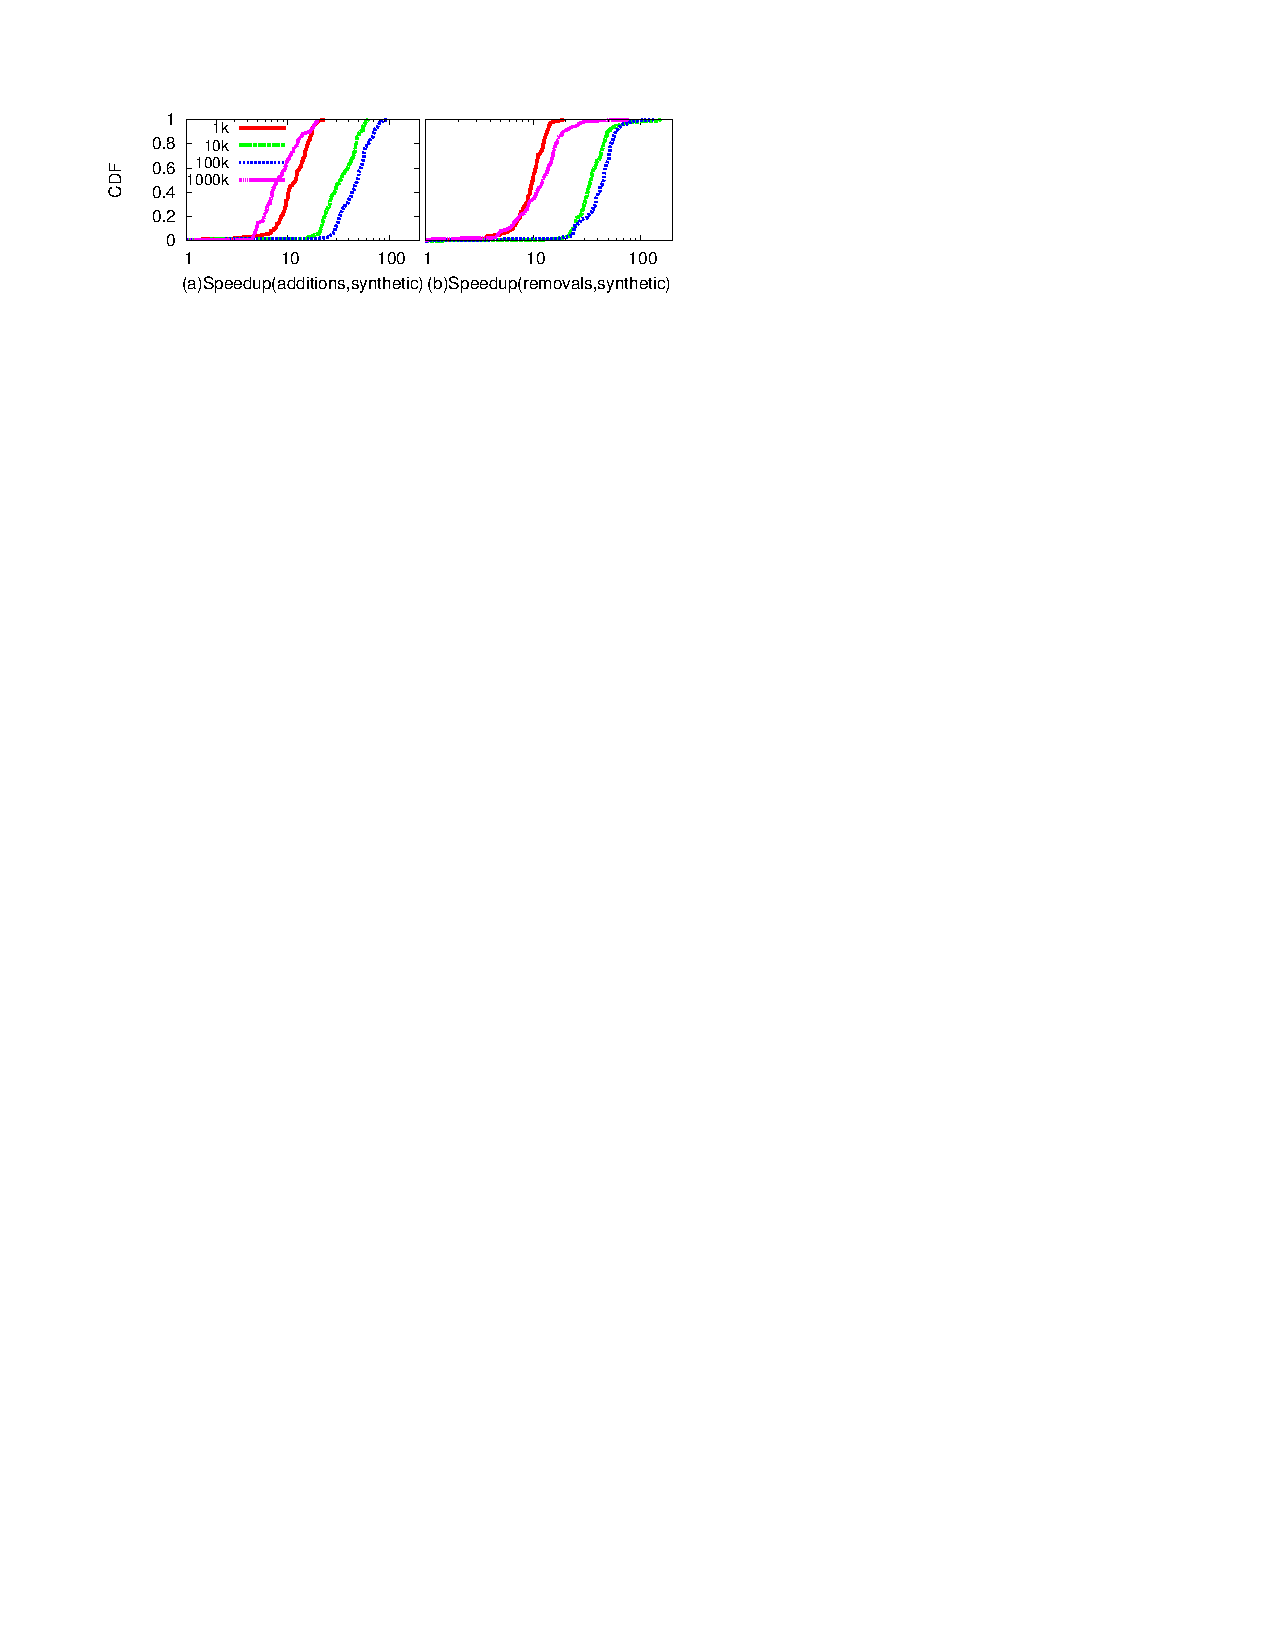
\includegraphics[width=\textwidth, height=0.3\textheight, keepaspectratio]{imgs/kdb-results21}
    \\ \qquad \quad
    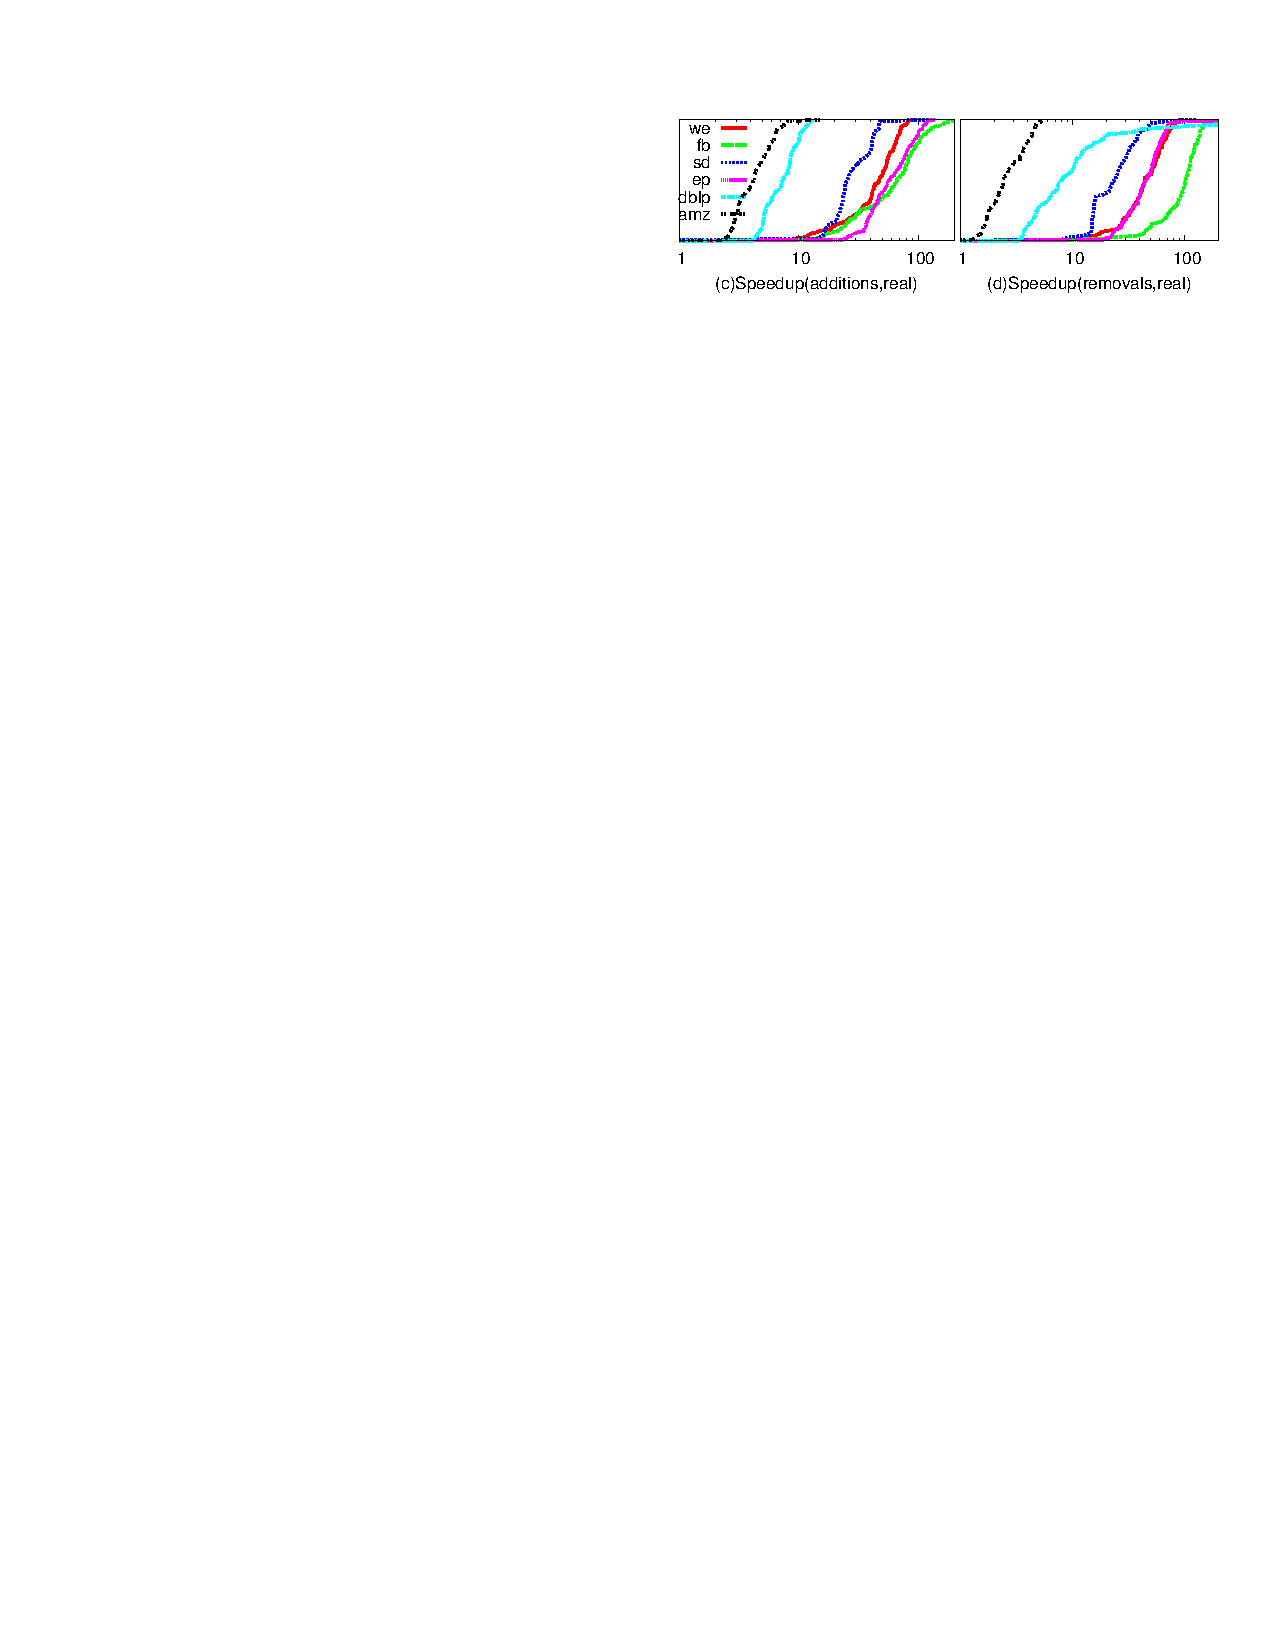
\includegraphics[width=\textwidth, height=0.3\textheight, keepaspectratio]{imgs/kdb-results22}
    \caption{Speedup over Brandes' for out-of-core version on synthetic and real graphs ($n = 1M$)}
  \end{figure}

  \begin{itemize}
    \item Out-of-core version scales up to 1M vertices
    \item Speedup up to 2 orders of magnitude
  \end{itemize}

\end{frame}

\begin{frame}
  \frametitle{Conclusions}

  \begin{itemize}
    \item Fully dynamic (addition and removal)
    \item Algorithm can scale to graphs with realistic size
    \item Ideal horizontal scalability
    \item $O(n^2)$ space bottleneck
  \end{itemize}
\end{frame}
